\documentclass[11pt]{article}
\usepackage[utf8]{inputenc}
\usepackage{geometry}
\geometry{a4paper, portrait, margin=2cm}
\usepackage[english]{babel} 
\usepackage{parskip}
\usepackage{chngcntr}
\counterwithin{figure}{section}
\usepackage{url}
\usepackage[noadjust]{cite}
\usepackage{mathtools}
\usepackage[nottoc,numbib]{tocbibind}
\usepackage{graphicx}
\usepackage{pdflscape, lscape}
\usepackage{array}
%\usepackage{textcomp}
\usepackage{gensymb}
\usepackage{tabularx}
\usepackage{caption}
\usepackage{everypage}
\usepackage{lscape}
\usepackage{amsmath}
\usepackage{mathtools}
\usepackage{enumitem}
\usepackage{algorithm}
\usepackage{algorithmic}
\setlist{noitemsep}

\title{An Evaluation of Cooperative Handheld Robotics in a Simplified 3D Construction Environment}
\author{Chris Meehan}

\begin{document}

\begin{titlepage}
	\centering
	
	
\includegraphics[width=0.6\textwidth]{bristol.png}
	\vspace{2cm}

	{\huge\bfseries The Design and Evaluation of a Novel Versatile Four Degree-Of-Freedom Cooperative Handheld Robotic Device\par}
	\vspace{1.5cm}

	{\Large\itshape By Chris Meehan\par}
	
	Supervised by\par
	Dr. Walterio Mayol-Cuevas
	
	\vspace{1.5cm}
	
	Department of Computer Science\par
	University of Bristol

	\vfill

% Bottom of the page
	{\large \today\par}
\end{titlepage}

\renewcommand{\thepage}{\roman{page}}% Roman numerals for page counter
\section*{Executive Summary}
\pagebreak

\section*{Acknowledgements}
\pagebreak

\renewcommand{\thepage}{\arabic{page}}% Arabic numerals for page counter

\setcounter{page}{1}% Start page number with 1

\tableofcontents
\pagebreak



\section{Introduction}
\subsection{Contemporary Robotics}
Advancements in the field of robotics have been plentiful over recent years, stemming from increased knowledge of the subject, improved processing power, as well as mechanical and material developments. As such, the capabilities afforded by robots have also increased, enabling a range of applications that, until recently, would not have been possible. As the area has progressed since its inception, it has naturally split into two distinct categories; external robotics and wearable technology. They are each characterised by the respective workspace in which they operate. This branching has appeared to come about due to typical robotic task requirements catering to either one or the other.

SIDE BY SIDE OF TWO ESTABLISHED FORMS OF ROBOTICS, WITH SPACE IN THE MIDDLE FOR `COOPERATIVE HANDHELD ROBOTICS'? XXXXXX

External robotics are distinctly separate from humans in terms of physical proximity. They are becoming increasingly common in large-scale industrial spaces due to their ability to provide improved efficiency and task precision through autonomy. A typical application is the automotive industry, in which production has been accelerated through the introduction of external robotics, performing specific assembly and painting operations, mostly in detached workspaces from the human workers. The other discrete area of robotics is referred to as `wearable technology', which, as implied by its name, is concerned with robotics that operate in the immediate personal space of the human user. This domain is typically associated with the augmentation of human actions, such as increasing physical strength or permitting certain motions that those with disabilities have been rendered incapable of. A well known use of this technology is the `exoskeleton', which can be tailored to accomplish either of these two functions through structural support and/or actuation.

However, both of these forms of robotics comprise inherent limitations, reducing their suitability to certain situations. As such, certain physical tasks exist that cater to neither domain. One case where this is evident is the \textit{tool space}. This area encompasses the typical range of tasks that humans have long since utilised passive tools to accomplish, along with exceeding performance possible by hand. This area is closely associated with flexibility, where unique tools can be used to deal with the same general task in various environments, or with completely different tasks altogether. Conversely, external robotics are typically limited to a rigidly defined workspace, performing very specific and repetitive tasks that they were designed for. Whilst wearable technology is more suited to this flexibility, it suffers from its limited adaptability to different users. Devices such as exoskeletons are very costly, and are uniquely tailored to individual body dimensions. This lack of generality equates to reduced applicability to the tool space, in which it is essential that other users are able to operate the tool when a certain individual is absent, or where a tool is marketed to a wide variety of customers.

\subsection{Motivation}
A proposed solution to bridge the gap between the two established forms of robotics, providing performance improvements in areas that neither are suited to, is \textit{handheld robotics}. This area aims to combine the key benefits of robotic efficiency and augmentation of human performance afforded by both fields, whilst maintaining the flexibility from human intuition in traditional tool use. Early work in this area has hinted at a wide range of potential applications where handheld robotics may excel, particularly in the fields of assembly, construction and maintenance/quality control. The fundamentals of their operation is that they cooperate with a human user, who in turn, positions the robot in a general location in which it can perform its desired operations, leading to improved performance. This sequence of events however, relies heavily on a key aspect of the device; its \textit{task knowledge}. 

Task knowledge refers to the robot being context aware, that is, it knows what operations need to be performed as well as the current state of progression through the task. This can act to alleviate the cognitive burden on the user, or to share it, with the user focusing on other aspects of the task than the robot. Most importantly, it enables a degree of cooperation between the user and device, in which the robot indicates its preference of simple actions to be performed by the user, such as repositioning it. In turn, the more precise or demanding operations are carried out by the device. Such a cooperation can lead to reductions in perceived workload by the user, be it physically or mentally, as well as improved task performance. This amalgamation of human intuitiveness and robotic efficiency through task knowledge may lead to unprecedented flexibility in the field of robotics.

The \textit{Handheld Robotics Project} at the University of Bristol has begun to lay the groundwork for the development of the field, investigating certain characteristics of two initial prototypes, namely the degree of cooperation with the user and the kinematics in general. This early work has warranted further investigation into the field, highlighting the potential for handheld robotics in general. As such, it is worth looking into alternative device configurations, whether in terms of cost, lead time, or general mechanical design. At such an early stage in its progression, further contribution to the breadth of the field can provide invaluable knowledge when developing it further, creating new devices or applications to improve their viability in the real world. As such, it was decided to design and build an alternative device to those existing currently, on a smaller time-scale at a reduced cost, and attempt to evaluate its performance. It is hoped this will shed more light on the potential of handheld robotics, as well as highlight areas of strengths and possible issues.




\subsection{Aims and Objectives}
The overarching aim of this project is to develop a new handheld robotic device and evaluate its performance in mentally assisting the user through task knowledge. As such, a new robot must be designed, assembled, and integrated with a control system so that it is fully operable. The functionality must be such that it enables a degree of performance evaluation. In order to implement this aim, a number of objectives must be met:
\begin{enumerate}
\item{Design a new handheld robot using CAD. The exact design will be achieved through an iterative process of prototyping via 3D printing and physical testing. Once fully designed and dimensioned, the robot should be constructed and assembled to connect to an off-the-shelf handle.}
\item{Develop a control system so that the actuation of the robot may be executed by a PC. This will entail using a microcontroller to sit between the robot and computer, receiving commands and controlling the actuation accordingly.}
\item{Interface the robot with an external optical tracking system, so that the position of the robot relative to target positions can be determined. This will utilise existing infrastructure at the University, namely the \textit{OptiTrack} motion capture system, and the libraries and API included will dictate that the development language will be C\#.}
\item{Implement an algorithm so that the robot may move to its intended target, or indicate the general position to the user when it is out of reach.}
\item{Perform a small evaluation of the robot's performance, this will comprise its ability to successfully indicate a desired position, its response to a varying target input and a small user study to assess its ability of alleviating cognitive workload.}
\end{enumerate}

\subsection{Added Value}
HERE OR IN ITS OWN SECTION IN THE BACKGROUND AND CONTEXT???XXXXXX

\subsection{Document Overview}
This thesis serves to cover the work accomplished throughout the project. Firstly, a background and context will be provided for existing areas of robotics in which the handheld domain may incorporate ideas or provide a potential improvement in the future. On top of this, a review will be provided of the current status of handheld robotics in general, with a focus on the work undertaken at the University of Bristol that is most relevant to this project. The design process of the robot will then be explained, along with the control system, the interfacing with the optical tracking system and the algorithm responsible for the robot's response to targets. Finally, the stages involved with evaluating the performance will be explained, and the corresponding results will be discussed.

\subsection{Summary}
NECESSARY TO HAVE A SMALL SUMMARY TO THE INTRO SAYING WHAT HANHDELD ROBOTS ARE AND WHAT IS HOPED WILL BE ACCOMPLISHED IN THIS PROJECT???XXXXXX
\pagebreak

\section{Background and Context}
\subsection{Robotics with Humans In-The-Loop} \label{intheloop}

Although robots have become vastly more capable over recent years with technological improvements, many tasks still require some form of human assistance in order for the objectives to be adequately met. Robots can be perfectly equipped to handle operations which involve precise motion or repetitive tasks, which may be present physical challenges to humans \cite{Chipalkatty2012}. Conversely, they still lack ability in areas which require the high-level cognitive reasoning that comes naturally to humans. As such, there exists many applications in which humans are in-the-loop for robotic operations. This applies to both forms of robotics that the handheld area sits between; external robots and, especially so, wearable technology.  

\subsubsection{Safety}

Perhaps the most important factor in these situations is how the robot receives and processes user intent. An input from the user should be analysed by the robot in terms of importance and the choice of subsequent actions should be made appropriately. A prime example of where this is of paramount concern is in vehicular operations, where potential accidents could be catastrophic. Anderson et al \cite{Anderson2010} investigated a semi-autonomous hazard avoidance framework and tested it in a real-life driving environment, where the human driver received full control during non-threat situations. However, in times of threat detection, the control system became fully autonomous and guided the car to the safety. In this situation, the robot assumed the expertise of hazard assessment and reaction time, whereas the human provided general navigation that was accepted by the system under normal circumstances. This is one extreme, where the human input is essentially ignored under certain conditions for the safety of the user and those nearby. 

The other end of the spectrum, human input must be immediately responded to in order to act safely, where it is assumed the human possesses greater threat detection. Thus safety to both the human and robot must be positively ensured \cite{Haddadin2007}. In industrial applications, the robot often operates in an isolated workspace from the human, where an extreme human input would constitute an emergency button or entering the workspace via a safety door/light gate, which the robot must respond to by halting all physical actions for human safety \cite{ISOGuards}. However, it is becoming increasingly common for the robot and human to share the same workspace, occasionally cooperating in a physical manner, such as the humanoid robot presented by Ott et al \cite{Ott2006} and illustrated in Figure \ref{figure:humanoid}, where parts can be passed between the robot and human.

\begin{center}
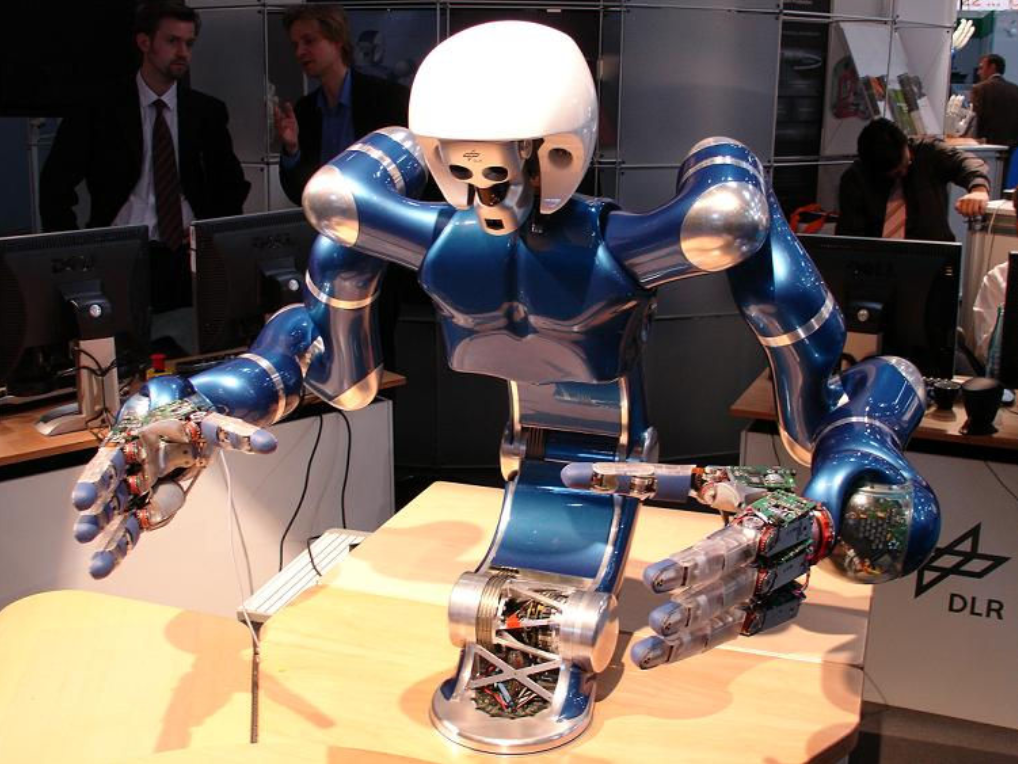
\includegraphics[width=0.48\textwidth]{humanoid.png}
\captionof{figure}{Two-Arm Humanoid for Dexterous Manipulation, image from \cite{Ott2006}.}
\label{figure:humanoid}
\end{center}

Existing operational requirements for collaborative robots have been specified in IS0-10218, which focus on defining the upper limit of either the tool centre point velocity, the dynamic power, or the static force. However, as discussed by Haddadin et al \cite{Haddadin2007}, these values are merely based on heuristics. As such, more specific severity indices were introduced, taking from biomechanically motivated quantities. In the case of this project, the robot was designed with the consideration of limiting the required dynamic power to suitable levels to be deemed safe as a collaborative robot. This entailed lightweight and flexible material design choices for moving part, greatly reducing any risk to a human user.

\subsubsection{Autonomy Study}
The reliability offered by human controllers can rarely be matched by autonomous agents. Similarly, the efficiency afforded by robots is highly attractive in physical tasks. Finding a strong balance between the two is essential in successfully accomplishing a task. Heger et al \cite{heger2006} investigate a mode of shared control, referred to as ``Sliding Autonomy". Fundamentally, this is an analysis to find the optimal flow of control between autonomous agents and a human operator for a given task, where an operator observes the operation and intervenes when necessary. A scenario was performed based on the model where three robots work cooperatively with a human operator to assemble a physical structure, with numerous failure modes deliberately implemented. The results indicated that the cooperation compromise resulted in task efficiency similar to a fully autonomous mode, while maintaining a level of reliability associated with teleoperation systems (remote human control). The constant attention of the human, without being cognitively demanding, improved the success rate while acting as a safety net for failures that the robot alone cannot recover from.

There are plenty of other investigations into the study of variable autonomy, such as in \cite{Dorais1999}, which looks into variable interactions in space missions, and in \cite{tambe2002}, which concentrates on the costs (time delays and other effects) of such transfer-of-control systems. Although this area of interchangeable control is mostly focused on with regard to external robotics, it is still relevant to the handheld field. As covered in \cite{GreggSmithDesign}, examining the varying degrees of autonomy that a handheld robot may exhibit for a given task is necessary to locate the control set-up to give optimal performance.
A different approach was taken to shared control in \cite{Poncela2009}, where the efficiency offered by both members in the cooperation was measured at each time instant from the point of view of reactive strategy. The experiment in this paper focused on the shared navigation of a Pioneer AT robot, where the commands of both the human and the robot were weighted and linearly combined, resulting in a single motory operation, as illustrated in Figure \ref{figure:autocar}.

\begin{center}
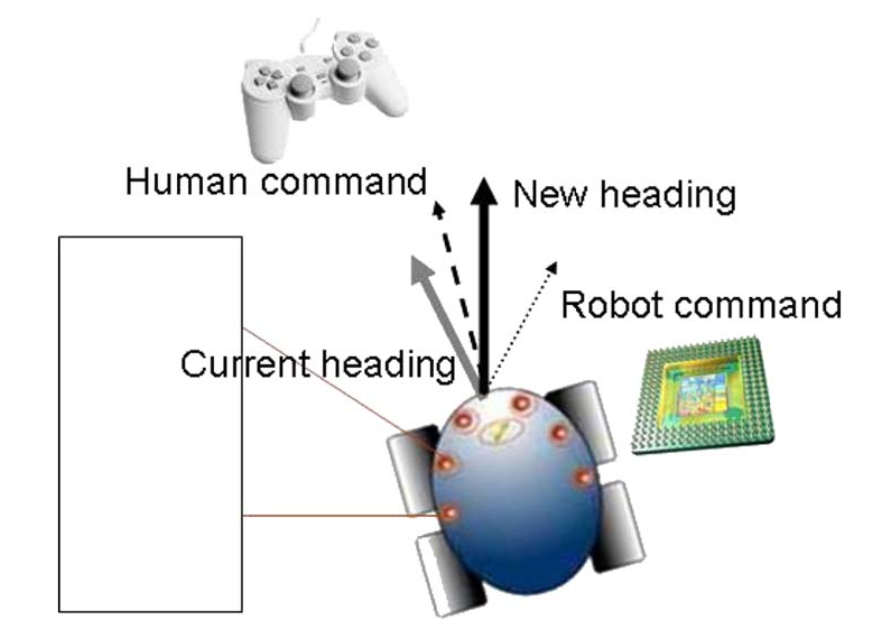
\includegraphics[width=0.48\textwidth]{autocar.png}
\captionof{figure}{Resulting command from human and robot inputs, image from \cite{Poncela2009}.}
\label{figure:autocar}
\end{center}

The results of this experiment showed that the weighting between the two inputs led to performance which, although not matching that offered by each member alone, did seem to combine the benefits of both when taking a range of scenarios into consideration. This is a rare situation in which the task at hand could be performed with equal skill by both human and robot, and caters to the speciality of neither. However, the approach of taking a weighting between the two inputs is interesting. 

It may be worth investigating such a method with handheld robots in the future. This would entail combining the two signals of human intention and task planning, and deciding the action based on the weighting the given scenario. This could add a degree of flexibility to the robot, adapting to new changes in the task, as identified by the human, or compromising between the two signals. With such a case, different settings could be explored by tuning the weighting given to each signal on a scale with a range of values, as opposed to just three discrete levels of autonomy as was the case in \cite{GreggSmithDesign}. However, such an investigation would require an extensive user study, with participants performing tasks repeatedly for a large variety of weightings. This is outside the scope of what is hoped the current project will achieve.

\subsubsection{Collaboration with Assistive Robotics}
Rather than replacing human operations, robotics can be employed to assist in them, maintaining human flexibility while increasing productivity. One such case where this is applicable is in the manufacturing industry, particularly assembly. Robots with highly specific purposes have long been used on assembly lines to increase output, performing simple and repetitive tasks at a faster rate than is possible with human workers. However, humans are frequently used for more complicated procedures that require motion in multiple degrees of freedom. The adaptability and range of motion of human workers is often unrivalled compared with traditional robotics, as well as being much more available. 

A sensible compromise is investigated in \cite{lenz2011}, where robotics are used to provide assistance to a human-oriented assembly task. A Hidden Markov Model (HMM) based analysis was used so that the robot may predict the next stages of the task, lending assistance by passing the required components to the user at the appropriate time so that they may continue with the operation. As a pre-requisite for any useful interaction between the human and the robot, the robot must first be trained. In order to accomplish this, the assembly tasks were performed solely by the human whilst sensors were used at various hand and body positions, so that the task motions could be adequately tracked. A similar study, focused primarily on the timing of assistance, contains an in-depth description of this preliminary set-up \cite{huber2010}. The task comprised the assembly of a six-block tower, bolting the blocks together in varying manners. Once the data was collected for the human performed task with sensors, the results were used to form the model.

The model generated in \cite{lenz2011} could then be transferred to the robotic platform JAHIR (Joint-Action for Humans and Industrial Robots). This hybrid assembly platform for the context outlined in the paper is illustrated in Figure \ref{figure:jahir}. Both the robot and the human share a designated workspace, whereas the storage areas for the parts are only accessible by the robot. An interaction area exists which overlaps with the human workspace, in which the robot may assist by transporting required parts to within human reach. There are numerous options for estimating the progress of human-performed tasks, one such technique is the one used for the preliminary experiment; strategically placed accelerometers and microphones. This technique is outlined in detail in \cite{lukowicz2004}, where most workshop activities could be identified at 84.4\% accuracy. In the case of the preliminary experiment in \cite{lenz2011}, pertaining solely to the assembly task, greater accuracies were achieved.

\begin{center}
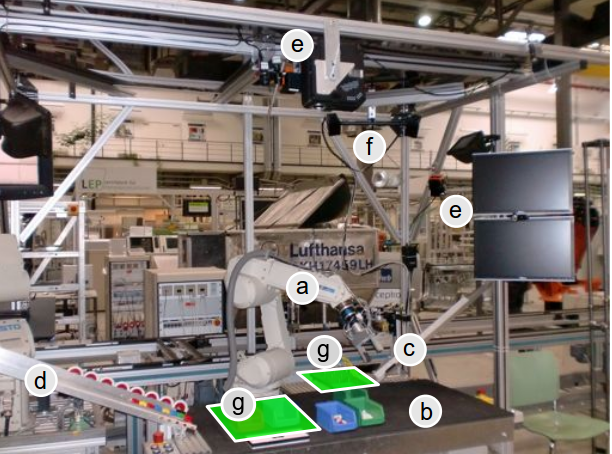
\includegraphics[width = 0.62\textwidth]{jahir.png}
\captionof{figure}{JAHIR assembly demonstration platform - a) Industrial Robot, b) Shared Workspace, c) Slide for Assembly blocks, d) Slides for Other Parts, e) Sensor Devices for Input/Output, f) ARTrack System g) Storage Space for Robot. Image from \cite{lenz2011}.}
\label{figure:jahir}
\end{center}

However, in reality, it is not feasible for assembly workers to wear a plethora of wired sensors while performing tasks. The physical and mental comfort is greatly reduced under such conditions, with the sensors creating a feeling of intrusiveness. A viable solution to this issue is the use of occupancy maps, which are commonly employed in robotics to determine position and motion, providing a robust approach to spatial perception and navigation problems. This technique, covered in depth in \cite{elfes1989}, was implemented for the robot assisted assembly task in \cite{lenz2011}, using the three-dimensional velocity, acceleration and jerk as input to the individual HMMs. This idea of measuring movement in physical space without excessive wiring is an essential component to the viability of handheld robotics, which have previously employed optical tracking from an external device as a solution. Other sensing methods will be explored in the future, with the aim of improved practicality in real-world scenarios.

This occupancy map method allowed for a recognition accuracy of 92.26\% for the right hand, comparable to the recognition rate of the reference experiment that relied on sensors. Therefore for the vast majority of the time, the system could accurately predict the task progress, and respond with the correct actions accordingly. The key here is that the robot must be context-aware. This enables much greater cognitive capabilities and a higher standard of interaction with the user. Cognitive Technical Systems (CoTeSys) is a group with a research focus on sensing and actuation in the physical world. As explained in \cite{buss2010}, this allows the robot to exhibit behaviours that suggest it can `learn'. The foundations of cognition in humans and animals are used to develop cognitive models, which can then be applied when designing control systems for more specific technical applications. 

The group uses a cognition-based perception-action closed loop as a basis for investigating cognition in technical systems, as illustrated in Figure \ref{figure:cognitivearchitecture}. This architecture focuses on five main areas; perception, action, knowledge, learning and reasoning. The model may be directly applicable to the field of handheld robotics. Task knowledge and the way in which the device receives and processes data from both the environment and the user, responding accordingly, bears many parallels to the goal of handheld robotics in general. Thus, such an architecture may be considered as a reference when designing applications for handheld robotics. 

\begin{center}
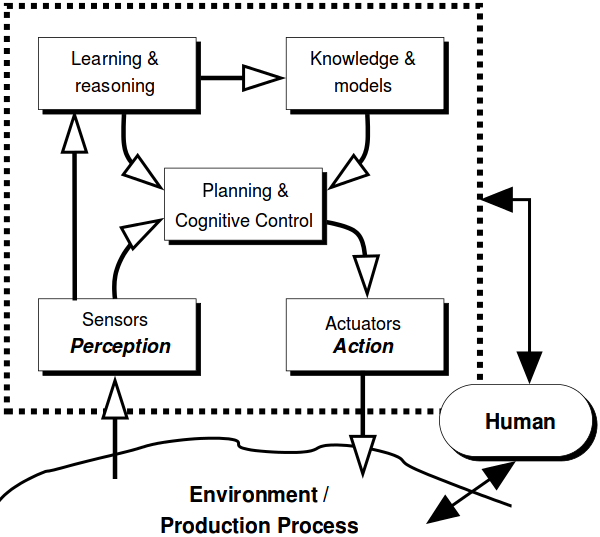
\includegraphics[width = 0.5\textwidth]{cognitivearchitecture.png}
\captionof{figure}{Cognitive System Architecture: Perception-Action Closed Loop, image from \cite{buss2010}.}
\label{figure:cognitivearchitecture}
\end{center}

\pagebreak














\subsection{Robotics in Building Environments} \label{building}

From a fully autonomous perspective, using robots in construction environments is becoming an increasingly attractive proposition. Although machines have been utilised to assist in construction since the industrial revolution, there has typically been little in the way of automation. With advancements in robotics, they may be incorporated into building applications to reach unprecedented levels of speed and efficiency. Numerous investigations and demonstrations have been carried out of robots performing assembly operations from a set of known requirements, corresponding to `task knowledge'. However, most of these examples are based around two-dimensional systems, such as manipulating blocks to construct flat structures, as in \cite{werfel2006}, not considering height.

The building and construction industry has been identified as an area of strong potential for handheld robotics. It is thus used as background to highlight examples where the introduction of a new field between the two established forms of robotics could prove worthwhile and beneficial. External robots, although able to possess task knowledge, are limited in this area in their ability to deal with changing requirements and their on-site mobility. Of course, the limitations of wearable technology remain their lack of adaptability to different users. These issues in particular may have a solution in handheld robotics. On top of this, the notion of unskilled workers being able to cooperate with such a device to accomplish a task may also have applicability to the construction area.

\subsubsection{Mobile Robots} \label{mobilerobots}
Petersen et al \cite{Petersen2011} present a hardware system in which a mobile robot manipulates blocks in three-dimensional space to match desired structures. As well as this, they also produced a high-level control scheme that could enable multiple robots to autonomously share the workload of a user-specified building task. The results were successful and the prototype robot constructed structures that were greater in height than itself, doing so via climbing, navigation and manipulation. This was accomplished without the need for complex sensing and control mechanisms by the design of the simplified interconnecting structural blocks and the way in which the robot interfaces with them, as illustrated in Figure \ref{figure:buildingrobot}. It has been suggested that there exists a future opportunity for a series of handheld robots and respective human users to work together to accomplish tasks of much higher complexity than possible from just a single device. This would bear parallels to the work in \cite{Petersen2011} in which the task knowledge is shared and updated between multiple devices accordingly.

\begin{center}
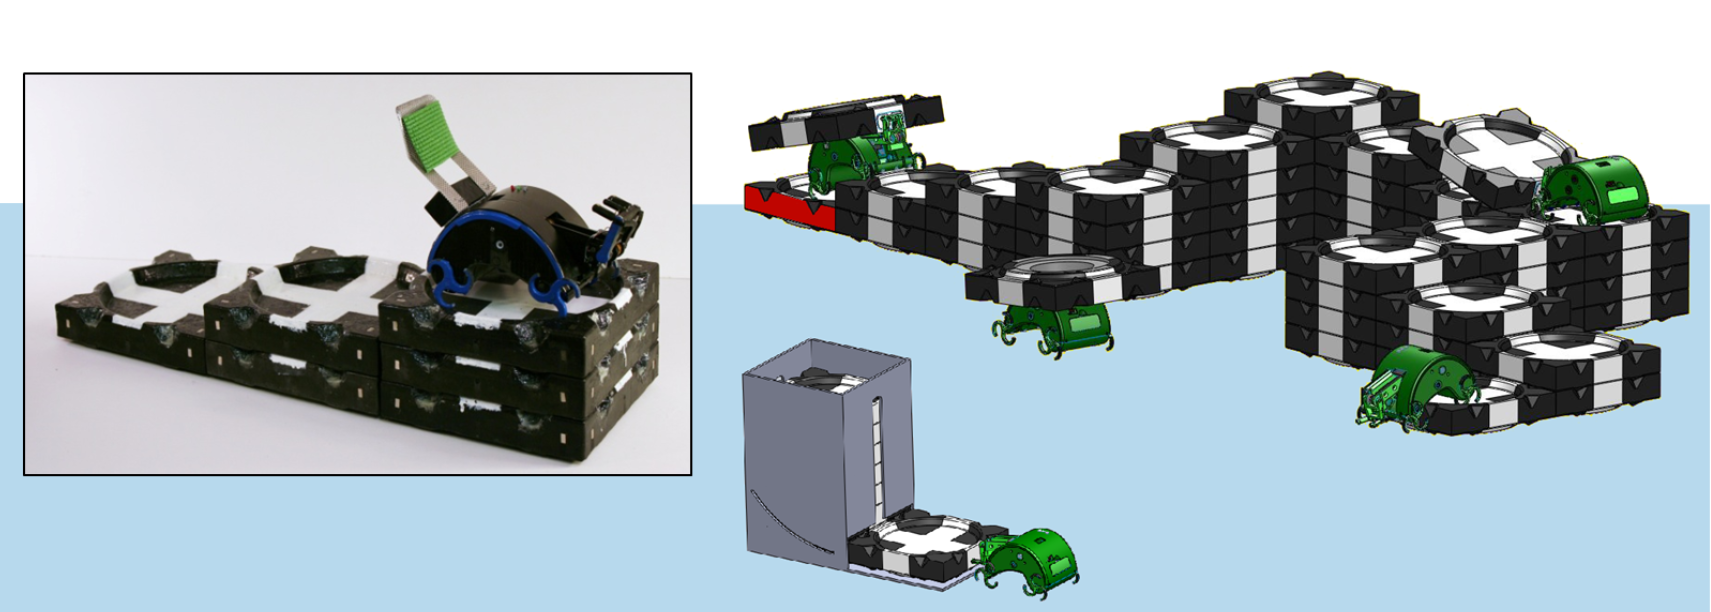
\includegraphics[width = 0.6\textwidth]{buildingrobot.png}
\captionof{figure}{Hardware system in which robot builds specified structures. Inset: Physical image of prototype atop six-block stricture. Outer image: Concept for system goal, in which multiple robots act together to distribute workload of a much larger structure. Image taken from \cite{Petersen2011}.}
\label{figure:buildingrobot}
\end{center}

This idea of designing the structure blocks in a passive manner so that they naturally fit together, reducing sophistication in orientation, provides a neat solution to overcoming positional errors. In this project, the physical experiments and tasks to be performed is not the sole focus, as a large portion of the scope is dedicated to the design and control methodology of a new device. However, future work will address the physical performance to a greater degree, and in such case, will likely take strong inspiration from such self-aligning building blocks as observed here. One common feature that is simpler to incorporate is the use of magnets for physical interaction with robot to block. Blocks in this project will likely have to be of a much larger scale due to the realistic accuracy expectations of the design in the short-term, thus cost reduction in terms of material and manufacture will be a large consideration.

\subsubsection{Drone-Based Assembly}
With recent developments in Unmanned Aerial Vehicle (UAV) technology as a whole, it is becoming increasingly viable to deploy rotary wing platforms to interact with the physical environment. The main advantage they offer over typical ground based alternatives is improved speed and accessibility with regard to hard-to-reach regions. Moreover, using rotary wing based UAVs, such as quadcopters, over their fixed wing counterparts, allows for a more controlled operation in a tighter workspace. The design and control associated with transporting a payload with such a rotary based UAV is presented in \cite{mellinger2011}. The paper looks at different gripper designs and how successful the robot was in estimating and manipulating the mechanics of the varying payloads. Several issues arise when using UAVs to transport payloads, namely the limited weight bearing capacity and the fact that the dynamics are altered when carrying payloads. 

The grippers investigated in this paper either operate by traditional clamping (impactive) or surface penetration (ingressive). However, the reduced motion of the fixed claws inevitably leads to more positional uncertainty during hovering. A solution is proposed in \cite{cano2013}, which covers the design of a 6-DoF aerial manipulator (see Figure \ref{figure:uavmanipulator}) for UAVs to assemble bar structures. This is made possible by developments in high power aerial platforms, reducing weight restrictions. The 6-DoF manipulator in the paper focuses on three main functions; the \textit{capture} (approaching and grasping the bar), the \textit{transport} (transferring load from storage to site) and the \textit{assembling} (installing to the structure).


\begin{center}
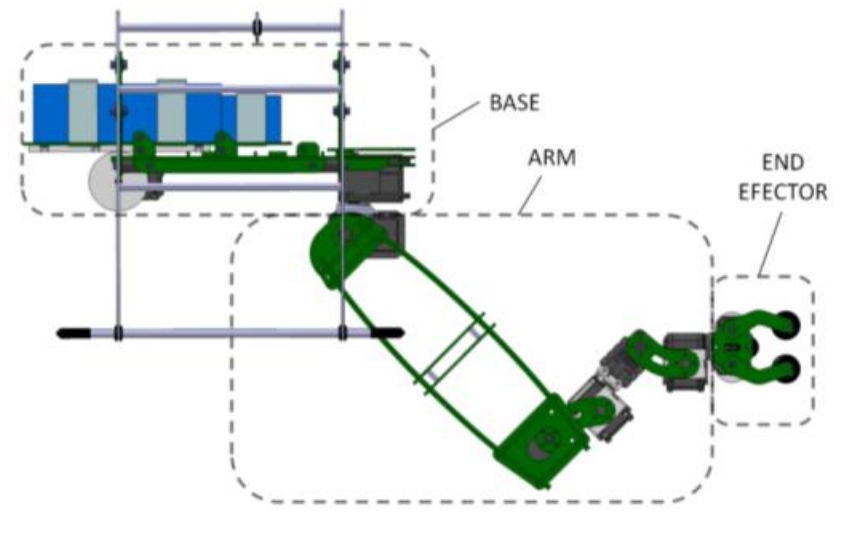
\includegraphics[width = 0.5\textwidth]{uavmanipulator.png}
\captionof{figure}{Components of Aerial 6-DoF Manipulator: Base, Arm and End Effector. Image taken from \cite{cano2013}.}
\label{figure:uavmanipulator}
\end{center}

Although this aerial design remains relatively untested in terms of control, it possesses similarities to the Mark II handheld robotic design in \cite{GreggSmithKinematics} (similar DoF but contains roll), and inspiration may be taken in the future when considering alternative end effectors for assembly-based tasks. This project aims to provide further groundwork and breadth in the design of new handheld robotics, with less focus on advancing the physical capabilities, and as such magnets are to be used for interacting with external bodies due to design simplicity. However, in the future when application and capabilities become more of a focus, new end effectors may be designed in tandem with specific assembly blocks, and each of impactive, ingressive, rollers or passive-jointed magnets would all be viable options.


The feasibility of using rotary UAVs to construct building-scale structures is explored in \cite{latteur2015}, in which a project is outlined that envisions an alternative construction approach similar to that observed in nature. This entails the gradual addition of more material to an existing structure in a safe and precise manner. Despite the energy considerations, it was concluded that large-scale construction may be possible through drones, with the potential improving in parallel with advancements in drone technology. An issue that was identified, as was also the case in Section \ref{mobilerobots}, is the level of precision required for typical construction that is finer than afforded by fully mobile robots. Certainly in the early stages of handheld robotics, this will be a key issue as well. In this project it is avoided by considering part dimensions based on the accuracy of the robot, not the other way round. 

This achievable accuracy problem is even more evident in aerial vehicles, and in \cite{latteur2015}, a similar solution was employed to \cite{Petersen2011}, mitigating positional imprecisions through the use of modular self-aligning components. Three different approaches were investigated for such a component; \textit{droxels}, conical interlocking \textit{dricks}, and rounded conical interlocking \textit{dricks}. These designs provide further inspiration for designing the assembly components for the handheld robotics construction task. In future development, when the capabilities associated with construction are more rigorously investigated, these self-aligning designs will be used as strong inspiration. However, due to the limited time-scale of this project and the comparatively smaller focus on assembly capabilities, such designs were disregarded in favour of plain blocks sized to meet the precision afforded by the new device.

KEEP THIS STUFF IN OR REMOVE???? ASK WALTERIO??? XXXXXXXX

\begin{itemize}
\item{Droxels (Drone Voxels) - Voxels are three dimensional pixels, different designs can lead to strong space-filling capabilities and allow for construction of complex shapes. They are somewhat more difficult to grasp and position but possess strong potential. One of the key issues is the manufacture complexity, with 3D printing being the most viable. See Figure \ref{figure:droxel}.}
\item{Conical Interlocking Dricks (Drone Bricks) - This option allows greater flexibility regarding positional tolerance. A lot of their potential lies in the fact that they can easily be constructed from more rigid structures such as concrete. However, unique blocks have to be designed to allow cornering. See Figure \ref{figure:cid}.}
\item{Rounded Conical Interlocking Dricks - Similar to the standard counterpart, except with a rounded shape and two full cones on top to allow for curved walls. See Figure \ref{figure:rcid}.}
\end{itemize}



\begin{center}
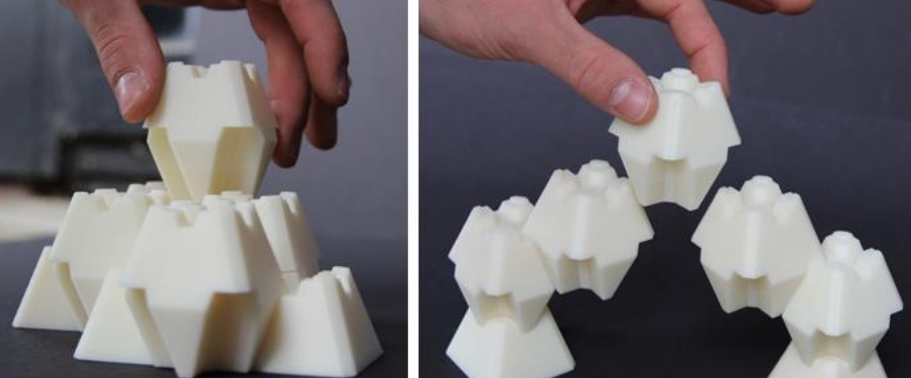
\includegraphics[width = 0.5\textwidth]{droxel.png}
\captionof{figure}{Droxel Design, image taken from \cite{latteur2015}.}
\label{figure:droxel}

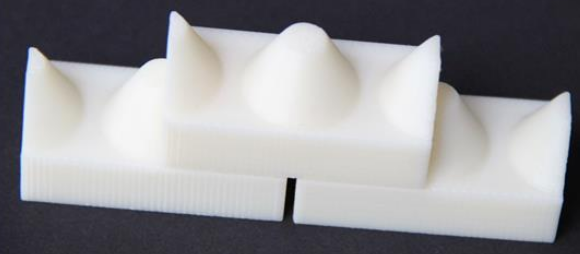
\includegraphics[width = 0.5\textwidth]{cid.png}
\captionof{figure}{Conical Interlocking Drick (CID), image taken from \cite{latteur2015}.}
\label{figure:cid}

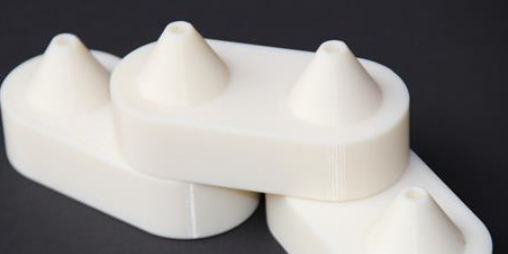
\includegraphics[width = 0.5\textwidth]{rcid.png}
\captionof{figure}{Round Conical Interlocking Drick (RCID), image taken from \cite{latteur2015}.}
\label{figure:rcid}

\end{center}



\subsubsection{Scene Knowledge}
One of the key considerations in robots performing construction tasks is how they navigate around the environment. The careful pre-planning of the construction environment is often necessary, so that autonomous agents can be informed of valid paths to avoid undesired collisions. Whole studies have been dedicated to this area, such as in \cite{Arkin1990}. In this paper, the autonomous agents are given prior knowledge of the environment as a whole and not just specific paths. This behaviour-oriented approach encourages vision/ultrasonic sensing to detect obstacles, reducing reliance on dead-set routes. Being more than fifteen years old, such techniques have become more established now, as in \cite{Petersen2011}. In many situations however, there is still a relatively strong dependency on a well defined environment, beyond just the relative locations of source/targets.

This reliance on environmental knowledge, as well as pre-planning of paths, is one of the areas in which handheld robotics can excel, providing an elegant solution to the guidance issues experienced by separate and autonomous robotics. As a user can transport and orientate a handheld device in any way they intuitively see fit, much greater flexibility is provided. The need for a rigidly defined environment and careful pre-planning, which is imperative to external robots, is vastly reduced with handheld robotic tools. Of course, fixed obstacles can still be made known in order to provide the most efficient movement. However, as the user is in full control of the general location of the robot, the user actively recognises and avoids obstacles with minimal cognitive effort. Hence this is an element of construction based robots that is of far less concern when designing new applications, further outlining the potential for handheld robotics as a whole. 

\pagebreak












\subsection{Handheld Robotics} \label{handheld}
\subsubsection{Medical Devices}
The field of handheld robotics has been largely unexplored in comparison to the established areas of robotics in which it sits between; fully external and wearable technology. The vast majority of the existing work in the handheld area is focused on the medical industry. Numerous surgical devices exist within this area, supplementing the skill and performance of the surgeon during precise operations. Payne and Yang \cite{Payne2014} review the existing and emerging trends in handheld medical robots, stating that the technical challenges differ from grounded robots in that miniaturising the devices is essential, whilst having multiple degrees of freedom is often less important.

An example of such a device is the handheld master-slave combined manipulator (MCM), developed by Matsuhira et al \cite{Matsuhira2002}, which offers added functionality to laparoscopic surgery that is not possible with conventional instrumentation. The design entails the addition of two degrees of freedom to the typical forceps, forming a cable-driven slave hand controlled by a master grip mechanism that houses two servo motors, as illustrated in Figure \ref{figure:masterslave}. The added yaw axes and the gripper end effector then enable internal suturing tasks, where potentiometers on the master grip interface with a notebook computer for controlling the motors. Other handheld robotics in the medical field include cutting implements incorporating haptic feedback (indicating force exertion) \cite{Payne2015}. There is also a significant amount of work regarding self-stabilising devices to compensate for physiological tremors, such as the  "ITrem" \cite{Latt2009}, which utilises sensing, filtering and manipulation to enhance surgical precision, or the mechatronic cup holder that alleviates the symptoms of Parkinson's patients \cite{Fischer2010}.

\begin{center}
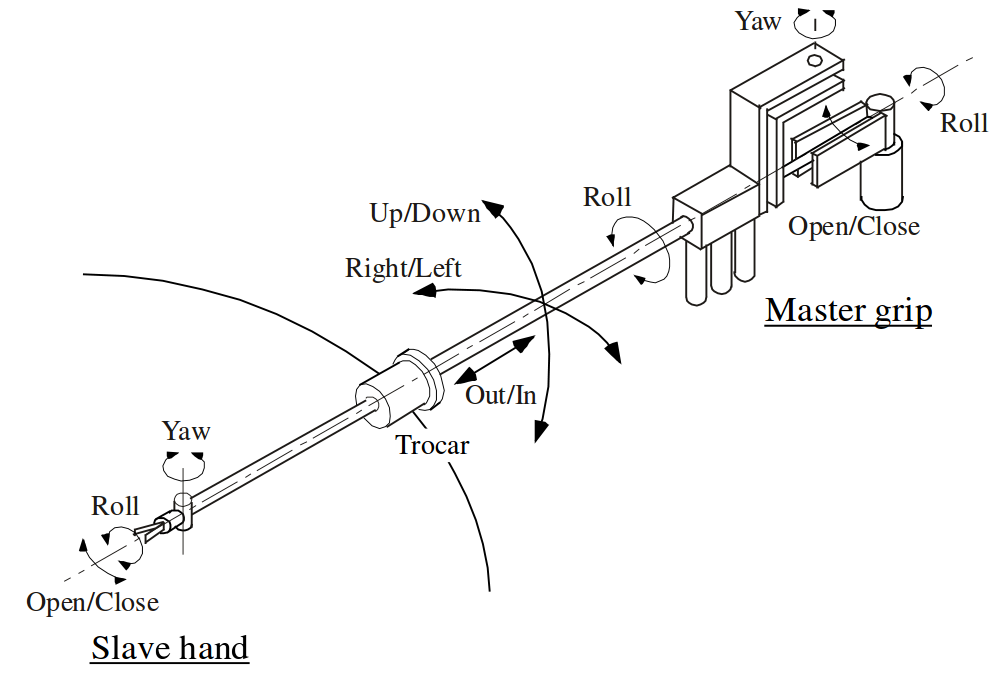
\includegraphics[width=0.5\textwidth]{laparascopic.png}
\captionof{figure}{Master-Slave Manipulator for laparascopic surgery, image from \cite{Matsuhira2002}}
\label{figure:masterslave}
\end{center}

However, up until 2015, there had been little research in the way of handheld robotics in the \textit{toolspace}. Tools have become a fundamental part of the way humans interact with the physical world, enabling the completion of tasks which would otherwise propose physical or mental challenges. They often allow operations to be performed that would otherwise be impossible, or simply reduce the task duration and workload, thus leading to an improved quality of life. One such example of work in this area is a handheld automated welding device, which enables welding to occur only when positioned correctly \cite{Echtler2004}. Although this constitutes an application of handheld robotics in the tool space, it is constrained by similar limitations to those present in the examples cited above when looking to classify this as a generalised handheld robotic tool that cooperates with the user. The aforementioned novel devices were designed with relatively few degrees of freedom and with very specific tasks in mind. This means that they are limited to single tasks, and cannot easily be adapted to alternative applications. The other key factor associated with the existing devices is their limited 'task knowledge', reducing the potential for cooperation between the device and the user.

\subsubsection{University of Bristol Handheld Robotics Project} \label{bristolhandheld}
Recent work undertaken at the University of Bristol has formulated the “Bristol Handheld Robotics Project”. This has focused on the potential of multi-degree-of-freedom handheld robotic devices operating in the tool space. A critical component of the research has been the capability of the robot to assume task knowledge for the desired procedure. The foundation for this branch of work was laid by A.Gregg-Smith and W.W.Mayol-Cuevas in \cite{GreggSmithDesign}, where a handheld robot was constructed and evaluated in terms of user cooperation. The underlying motivation of the paper was the assertion that there exists a much greater potential for handheld robotic applications than just the medical industry.

The work in \cite{GreggSmithDesign} covers the development of a four degree-of-freedom (4-DoF) prototype handheld robot, in which the aim was not to design a robot which can surpass human capability, but rather to evaluate the cooperation between the user and robot for various degrees of autonomy. This design and evaluation here has certainly laid the groundwork for future development of handheld robotics. The arm comprises a carbon-fibre backbone, and is cable-driven by two pairs of motors and pulleys located in the base; one opposing pair providing a degree of freedom each to the midpoint and the tip, with the other pair providing a second degree to each point, as illustrated in Figure \ref{figure:mark1}.


\begin{center}
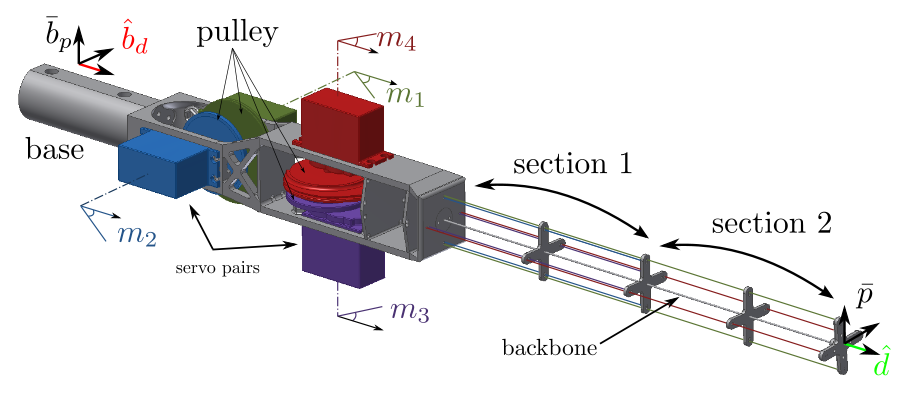
\includegraphics[width = 0.6\textwidth]{images/mark1.png}
\captionof{figure}{CAD model of the Four Degree-of-Freedom Mark I robot, image from \cite{GreggSmithDesign}.}
\label{figure:mark1}
\end{center}

The design takes inspiration from [31] which, unlike typical cable-driven designs, employs one motor
to provide tension to a pair of opposing wires, which reduces the motor count to DoF ratio from 3:2 to 1:1. 
An external computer is used to interface with the servomotors and the trigger, responding to external
cues or program instructions by providing the necessary motion. In order to locate the robot spatially, an OptiTrack system made up of six strategically mounted cameras is
used to provide motion tracking, identifying the retro-reflective markers mounted on the robot. This
provides an accuracy of 0.2mm, although it was stated that the future aim would be to employ
on-board sensors for portability and practicality.


In order to calibrate the robot, it was necessary to perform kinematic modelling. Conventional forward
kinematics methods were not applicable to this design due to the non-linear interaction between sections 1 and 2
of the carbon-fibre backbone, shown in Figure \ref{figure:mark1}. As such, a regression based method was employed.
This entailed sending a wide range of commands to the arm and recording the resulting pose with the
motion tracking equipment. In total, 14641 vectors of motor angles were sent, with the corresponding
poses comprising a relative tip-to-base position and direction. A regression technique
was then used on the results to interpolate between the points to acquire estimated poses for unrecorded
motor vectors. This is covered in more detail in Section XXXX.

MENTION K-D TREES HERE FOR ACCELERATED SEARCH AND IMPROVED COMPUTATIONAL TIME, OR MENTION IT LATER ON IN THE CALIBRATION SECTION AS AN OPTION AND FUTURE IMPROVEMENT????XXXXXX


It is important to note that due to the limits
of the carbon-fibre backbone, the arm cannot self-intersect, therefore it is safe to interpolate
between the motor angles.

Inspiration was taken from this Mark I design in the development of the newer, flexible tube-based model, and naturally, similarities will be observed between the set up and control processes and the external infrastructure to interface with the robot and provide track motion. The key differences originate from the different arm material/structure, having a chain reaction of required design changes. Also, with the benefit of hindsight, design and material choices that hindered this Mark I design could be avoided, while strong points could be adapted. An example of this is the issue of the friction from the cables wearing through the base material. This led to the choice of an ultra low-friction cable material, and a stronger base material, using PLA over ABS. 

ALSO MENTION SIMILARITIES WITH THE TLX STAGE IF ANY OF THIS GETS COMPLETED IN PRACTICE XXXX

 , as well as the techniques used to quantify the task performance an perceived effort. 
 
Subsequently, a more advanced six degrees-of-freedom device was constructed over a longer period of time, as covered extensively in \cite{GreggSmithKinematics}. This design comprised distinct solid sections connected by links, as opposed to a continuous backbone, to allow for a greater range of motion. Originally, this project's objectives comprised the design and evaluation of new applications for this device. However, the robot experienced an improbable critical failure during a capability demonstration, rendering it unrepairable within the project time-line. As such, the new direction was taken regarding the design and construction of a simpler four degrees-of-freedom device and the corresponding evaluation. Hence the details of the Mark II device have become largely irrelevant in terms of this project, and will therefore not be covered. Both the Mark I and II devices are made openly available at \cite{handheldrobotics}.

\subsubsection{New Design Inspiration}

Given the relatively small time-frame of this project in comparison to those typically associated with the development of new robotic devices, it was necessary to design the robot so that it may be built and evaluated within this period. As such, some initial decisions were made at the start of the design process. The first was that the robot was to be cable driven, due to already possessing four high torque servomotors that have been proven to be reliable and effective on an existing prototype. The other choice was for the arm to be of singular solid piece of material, mitigating the design complexity associated with numerous links. As such, the design began to take shape as a four degrees-of-freedom cable-driven device. 

There are numerous existing designs that incorporate a single structure, cable driven arm, such as those covered in \cite{godage2011} and \cite{zhang2011}. However, these designs relied on a method in which each connecting cable was driven by a single dedicated motor. This was improved upon in \cite{yoon2009}, where a design was introduced that uses a single motor to drive a pair of opposing cables. This design was the inspiration for the first handheld robot prototype, as covered in \cite{GreggSmithDesign}. Given the similarities in the general design principles and handheld nature, inspiration was taken from the first prototype in the development of the new device.

However, one area identified for potential improvement associated with the designs in \cite{godage2011}\cite{zhang2011}\cite{GreggSmithDesign} was the possible range of motion. All of these designs involve a solid carbon-fibre backbone, which, whilst affording rigidity and a degree of flexibility, has natural limits on its deflection before snapping. Thus a maximum range of motion in the first prototype was found to be about $\pm$20\degree of each motor from the starting straight-arm position. This value was determined during the development stage as the carbon-fibre rods were found to snap with larger angles. As such, a new material for the arm was to be used, giving it discernible characteristic differences from the first prototype, with the hopes of achieving a greater range of motion whilst reducing vulnerability to damage on sudden impacts.

In \cite{reinecke2016}, an investigation was undertaken into a continuous elastic spine, actuated by tendons. This serves as an alternative to typical spinal structures which are stabilized by, or the equivalent of, intervertebral discs, muscles, and ligaments. The variation between structures with a finite number of links and elastic continuums is illustrated in Figure \ref{figure:robotVariation}. In this paper (\cite{reinecke2016}), a multiple DoF prototype is presented to demonstrate the possibility of different tendon routing configurations and elastic continuum shapes. One of the key benefits highlighted here was the fact that such structures address the problem of collisions. Robots that interact with humans and the physical environment must be able to withstand intended or accidental impacts without damaging the environment or the robot itself. Such impacts are damped with a passive elastic element, enabling work in unstructured environments. This robustness to impact was verified in \cite{reinecke2016} with external impact tests to both rigid and the elastic continuum structures proving that rigid mechanism experience two times the force under similar collision conditions.

\begin{center}
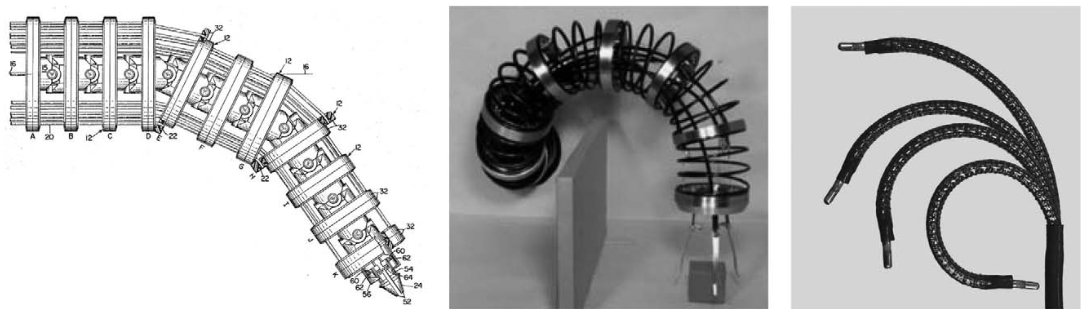
\includegraphics[width=\textwidth]{images/robotVariation.png}
\captionof{figure}{(Left) The hyperredundant Tensor Arm of Anderson and Horn \cite{anderson1967}, having a large number of linkages to increase flexibility. (Centre) The first sustained research program in continuum and hyperredundant robots, image from \cite{hirose1993}. (Right) Modern continuum robot used in medical applications, image from \cite{camarillo2008}. Note that all images were adapted from \cite{webster2010}, which reviewed existing robots in this space.}
\label{figure:robotVariation}
\end{center}


The other key advantage offered by elastic continuum arm structures is the greater range of motion as a result of their continuously bending nature. Further investigation into the design and modelling of such structures in a robotic context is provided in \cite{webster2010}. Inspiration, like much of robotics, has been taken from nature, where extreme manipulation and dexterity capabilities are exhibited by the likes of snakes and octopus tentacles. In this paper, multiple mechanical continuum robot architectures were reviewed, outlining the advantages over robots with a finite number of rigid links. At present, continuum robotics are relatively unexplored in comparison to more established rigidly linked structures, though it is predicted that their accelerating progress will lead to increasingly practical solutions in the future. For these reasons, which are highly applicable to handheld robotics (human/environment interaction and increased motion), it was decided to use a continuum elastic structure for the arm of the new design. This offers a fundamental difference between the first prototype, and provides added breadth into the field of handheld robotics in general.




\subsection{Designing Experiments for Handheld Robotics} \label{designingexperiments}
At such an early stage in the development of handheld robotics, it is essential to carry out experiments that reveal as many details as possible, contributing to existing knowledge that may be used as reference as the field in general progresses. Focus must be placed on important factors such as how well the user and device cooperate, how the desired actions of the robot are communicated to to the user and the benefits of using the device in terms of perceived effort and performance. The earliest experiments undertaken focused on evaluating the cooperation between the human and robot. Other experiments include investigating the effectiveness of different feedback methods for the robot in communicating desired positions, as well as the kinematics and motion performance in general. In the first two instances following, the cooperation was highlighted by the performance associated with three different levels of robot autonomy.

\subsubsection{Painting Task}
The painting task from \cite{GreggSmithDesign} entailed users being shown a template pattern on a screen and assigned with tracing the pattern with ``virtual paint". The motion capture system would register the position and orientation of the tip of the arm to establish the absolute direction of the painting. Then, a `key action' (user or program oriented action associated with progressing the task)would result in virtual painting, changing the colour of the pixels that the tip is pointing to. 

In both manual and semi-autonomous mode, the key action was a user oriented cue, in this case the pressing of the trigger to initiate painting. The manual mode involves a straight arm with the paint turned on with the trigger, while the semi-autonomous mode draws upon the pre-programmed task knowledge to enable movement along paths of contiguous pixels in the same target region while the trigger is held. However, it cannot move across gaps to unpainted regions by itself, requiring the user to reposition the tip. Alternatively, the fully autonomous mode involves the robot initiating and halting the painting action where it deems appropriate, providing the key action itself. This task setup is illustrated in Figure \ref{figure:painting}.

\begin{center}
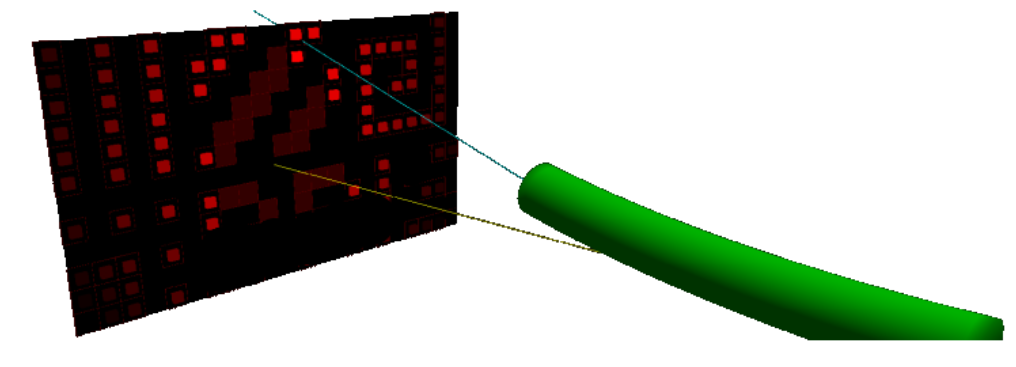
\includegraphics[width=0.5\textwidth]{painting.png}
\captionof{figure}{Model of painting task setup in autonomous mode (lights indicate preference of subsequent motion), image from \cite{GreggSmithDesign}}
\label{figure:painting}
\end{center}

\subsubsection{Tiling Task}
The tiling task, also from \cite{GreggSmithDesign}, involved fitting the end-effector with an electromagnet and picking up red or black tiles from designated hoppers before placing them in a predefined chequerboard pattern, as illustrated in Figure \ref{figure:tilingtask}. The magnet is activated/deactivated by pressing the trigger, except in the case of full autonomy in which the robot fully provides the key action, controlling the magnet as necessary. In manual mode, the absence of task knowledge means the arm remains straight, responding only to the trigger press with the magnet activation. In this case, it is possible for the user to provide an incorrect pattern, therefore a template was made visible so that all users performed the task correctly. 

In the two modes that comprise task knowledge, the arm moves towards the nearest hopper that it knows will provide a suitable colour, before moving towards the nearest suitable empty space on the board. In both cases, the robot will refuse to perform an action that conflicts with the task specification. In the case of full autonomy, the electromagnet is also controlled by the robot. Thus the tool will keep seeking to perform necessary actions, gesturing to the user where it should be positioned to do so, until the task is complete.

\begin{center}
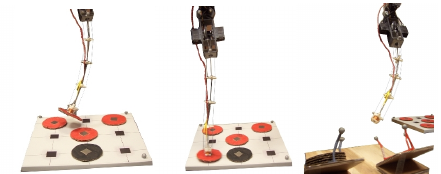
\includegraphics[width=0.65\textwidth]{tilingtask.png}
\captionof{figure}{Pick and Place Tiling Task with tip of first prototype, image from \cite{GreggSmithDesign}}
\label{figure:tilingtask}
\end{center}

The results from the previous two tasks indicated that the completion time was significantly improved with increasing degree of autonomy. The accuracy of the tasks however, showed little difference among the different modes. This was to be expected as the robot end effector was designed with an accuracy comparable to that of a human. The combined Task Load Index (TLX) scores also showed improvement with increasing autonomy, indicating that introducing cooperation with the robot reduces the perceived task effort. The individual TLX scores for various factors are shown for both the painting and tiling tasks in Figure \ref{figure:tlxscores}.

\begin{center}
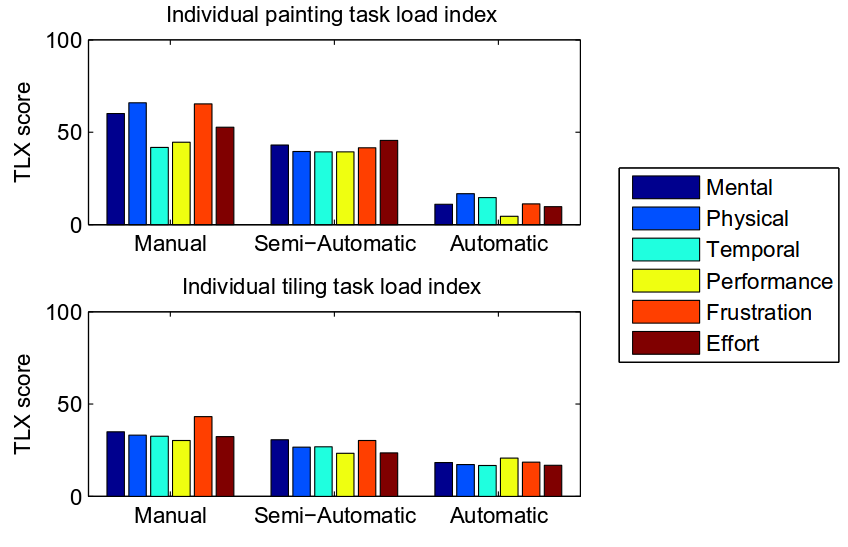
\includegraphics[width = 0.75\textwidth]{tlxscores.png}
\captionof{figure}{Individual TLX scores for both the tasks, image from \cite{GreggSmithDesign}}
\label{figure:tlxscores}
\end{center}

As the task accuracy exhibited little difference among the modes, and the completion time and perceived effort showed improvement with task knowledge, it was concluded that the users cooperated well with a task-aware handheld robot, where introducing levels of automation had a positive impact on essential elements of task performance. Although sharing elements of the task among the user and robot did not negatively affect performance, maximum overall benefit (accounting for perceived effort) was attained when the robot was given full control. Of course, there is still a strong element of cooperation in this scenario as the user must move the robot to its desired location, responding to its gestures accordingly.
	
\subsubsection{Spatial Guidance Task}

Manoeuvring the robot to a specific location so that it may perform its duties is an essential element of strong cooperation. Without effectively conveying desired locations in order to proceed with the task, the usefulness of the robot is severely hindered. Thus, some form of guidance is necessitated. Fitt's law is an established method of estimating the time to reach a known destination \cite{fitts1954}, and although was originally created with a 2D perspective, it has been extended to a 3D environment, such as in 3D pointing tasks \cite{Cha2013}. In either case, the way in which information is presented to the user from a human interaction point-of-view has often been considered to affect performance \cite{soukoreff2004} \cite{MOTOYUKI1995}. 
  
As covered by A.Gregg-Smith and W.W.Mayol-Cuevas in \cite{GreggSmithFeedback}, various methods were investigated in which the robot provided spatial feedback to the user during a 3D guidance task, using the more advanced 6-DoF device as mentioned in SECTION XXXXXXXX. The task comprised positioning the robot so that the end effector could be aligned to within 5mm and 5 degrees of a target pose for at least 200ms. The target pose took place at a range of locations on a small side table, and was also performed with a stand-alone handheld wand in order to evaluate the benefit of using the robot in a performance and feedback sense.

The seven conditions investigated are listed below, with the experimental set-up for the robot with virtual reality illustrated in Figure \ref{figure:vrrobot}.
\begin{enumerate}
\item{Robot provides gestures by pointing to location}
\item{7 inch 2D screen mounted to robot, showing wireframe model of table and target point}
\item{7 inch screen held in one hand, performing task with wand in other hand}
\item{Augmented reality headset (with transparent lense) while using robot}
\item{Augmented reality headset while performing task with wand}
\item{Virtual reality headset while using robot}
\item{Virtual reality headset while performing task with wand}
\end{enumerate}

In each case, an infra-red optical tracking system was used with retro-reflective markers attached to the key objects; the arm, wand, table, augmented/virtual reality headsets and the 7 inch screen. This allowed the pose of the robot to be calculated.

\begin{center}
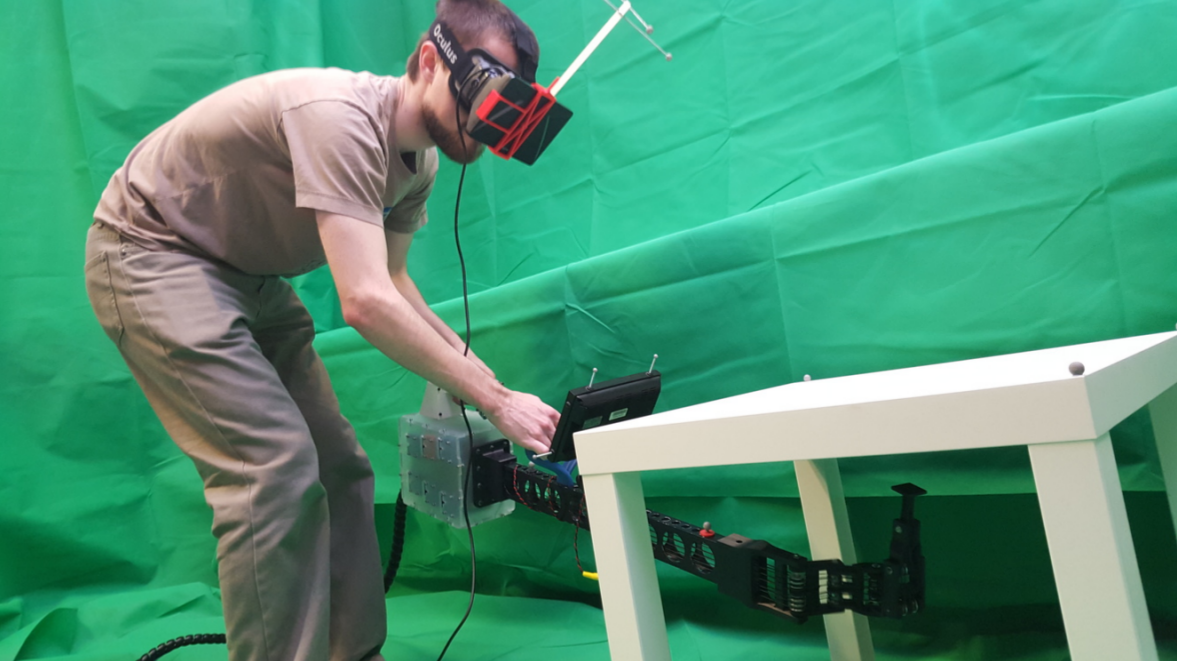
\includegraphics[width=0.55\textwidth]{vrrobot.png}
\captionof{figure}{Spatial guidance task being performed with the handheld robot where feedback is provided via a virtual reality headset, image taken from \cite{GreggSmithFeedback}.}
\label{figure:vrrobot}
\end{center} 
 
The robot itself possessed a 6-DoF pose in world space, while the joint angles constitute a further six DoF, resulting in an overall 12-DoF pose. Solving from one of these fully defined poses to another is computationally expensive, requiring minutes to be calculated where sub-second times are needed for a responsive tool. In order to overcome this issue, the path planning ability of the human was exploited, reducing the robot path-planning problem to 3-DoF. A variant of informed Rapidly Exploring Random Trees (RRT*) \cite{Gammell2014} was then produced in \cite{GreggSmithFeedback} to calculate the shortest route from robot to target, using the frame of reference of the target as the root of the tree. Once such a trajectory is known, the robot can use it to gesture along the absolute line as one of the feedback methods, as well as searching for a valid solution, as explained in \cite{GreggSmithKinematics}. This algorithm was always run during robot use, regardless of the feedback method.

The results of the completion time and the TLX combined scores in \cite{GreggSmithFeedback} indicate that all forms of feedback (augmented reality, virtual reality, mounted screen and gesturing) are shown to improve performance compared to the handheld wand. Although the gesturing mode itself does not show as great a performance difference as the visual methods, it does show an improvement nonetheless, justifying it as a viable option. As such, feedback through gesturing was the chosen option for this project, given its feasibility in the time-frame compated to the alternatives. The visual feedback methods themselves exhibited little difference between them. These strong results demonstrate the effectiveness of the robot in assisted tasks, outlining its potential for use in the tool space.
	
\subsubsection{Added Value}

TALK ABOUT ADDED VALUE OF DESIGN AND EXPERIMENT IN GENERAL. IE DEMONSTRATES THE DESIGN PROCESS THOROUGHLY FOR THIS TYPE OF FLEXIBLE TUBE CABLE DRIVEN ARM, ALLOWING OTHERS TO FOLLOW SUIT. ALSO SHOWS HOW THE FLEXIBLE TUBE IDEA IN GENERAL WORKS, ADVANTAGES AND DISADVANTAGES AS THIS HAS NEVER BEEN TESTED BEFORE. THEN OF COURSE ANY EXPERIMENTAL DETAILS. FURTHERS THE KNOWLEDGE OF HANDHELD ROBOTICS IN GENERAL AND ISSUES, AREAS OF OPPORTUNITY IT MAY FACE, PARTICULARLY FOR A CHEAPER, SHORTER TERM DESIGN THAN THE FULL 6 DOF MODEL

The objectives of the current project entail interacting with physical objects in a 3D representative environment, which differs from the physical interaction task performed in \cite{GreggSmithDesign}. The tiling task, although in reality involved relocating 3D objects, can be represented by a 2D environment. The task knowledge did not involve the depth of the tiles, and therefore they could be assumed to be a perfect disk with zero depth. The user would lower the robot until the discs were picked up or placed, whereas the two dimensions the robot focused on were in the x and y axes; lining up the end effector with the centre of the chequerboard positions.

Alternatively, this project aims to evaluate tasks performed in a 3D rich environment, interacting with objects of known width, height and depth, which must be placed accordingly to simulate a simplified construction environment. A different end effector will be designed, and although it may possess similarities to that used in the tiling task (electromagnet based) it will require an alternative mechanism to consider true 3D space. That is, the alignment of the objects will be important so the end effector must be such that different angles of approach will not cause alignment issues. Moreover, the work in \cite{GreggSmithDesign} focused more on generic tasks that would require no specific skill and be of little difficulty to the average person. As this project is investigating a more definitive scenario (building environment), the robot used in the new tasks will likely possess task knowledge and capabilities exceeding those of an unskilled worker. This coincides with the idea of enabling complex task completion by those without conventional training in that area, such as crowd-sourced building projects.

The spatial guidance experiment in \cite{GreggSmithFeedback} has yielded useful information regarding the development of handheld robotics in general, considering the importance of effectively conveying preferences to the user. For the current project, the guidance provided to the robot to the user will certainly play a big part in performing the experiment. This is especially so if mental attributes are added to the task to make it harder for the user to complete without assistance. Thus, if the tasks contain elements where the target objects are not immediately visible to the user, one of the three visual feedback methods demonstrated in this paper can be used with confidence. The use of the path planning algorithm in \cite{GreggSmithFeedback} to come up with a suitable 5-DoF pose will also be a key component of the new experiment.


\subsubsection{Task Load Index (TLX) and Perceived Effort}

When investigating task effectiveness, it is essential to quantify the perceived workload of the performer. This is especially true when researching methods that may improve the task performance. The established means of this quantification is the use of the NASA TLX (Task Load Index). A multi-dimensional scaling was introduced in \cite{hart1988} under the belief that subjective workload is in fact measurable, and has since become widely accepted. Subjective responses can thus be reliably evaluated to meaningful ratings. The six key rating scales associated with the index are mental demand, physical demand, temporal demand, performance, effort and frustration level. 

This TLX methodology was employed on each of the experiments that have been carried out for handheld robotics thus far \cite{GreggSmithDesign} \cite{GreggSmithFeedback}, yielding valuable information regarding the subjective workload of cooperative tasks with the robot. As such, it is logical that a similar technique will be used on the new experiment. An ethics approval agreement is already in place that will span the duration of the project. This will allow the undertaking of studies with human participants, concluding with them filling out a TLX form. 
\pagebreak




\section{Summary}

NEED TO DELETE THIS AS NOT RELEVANT, WILL BE A CONCLUSIONS AND/OR SUMMARY AT THE END OF THE DOCUMENT???? XXXXXX

A review of existing literature was carried out in order to better understand the area in which this project aims to contribute to. Most notably, the current work regarding handheld robotics at the University of Bristol was looked into. This is especially relevant as it formed the groundwork on which this project will be based,  providing crucial details of the apparatus that will be used. Particular focus was given to the design process which has led to the robot's current state and the evaluations of its performance and cooperation. 

Coinciding with this is the kinematics information on which the current robot is based. It was necessary to understand this as the approach used for the robot control will need to be exploited to perform any task scenarios which make up the evaluation. The recent study on the methods of feedback for the robot in \cite{GreggSmithFeedback} has enabled confidence when choosing how best to convey spatial information to the user. This is of obvious importance, as the robot will have to interact with the user to to indicate where it should next be located during the task, regardless of the specifics of the experiment. It may also become more pertinent throughout the development, if objects are out of line of sight.

A brief review was performed of the field of human in-the-loop operation. Despite being mostly based around external robots that require human input, it still provides useful insight into the way that humans interact with shared robotic tasks. An area of interest that was found dealt with `sliding autonomy' in which the degree of autonomy the robot exhibits can be fine tuned in a system of transfer of control. This led to improvements in task performance by combining the efficiency of the autonomous agent and the reliability of the human perspective, aiming to determine an optimal balance. This may be worth investigating in the future as a means of potentially locating a more efficient degree of autonomy for certain tasks. 

Another approach taken dealt with the weighting of inputs, in which both the human and the robot provided an input, and the singular operational result was formed of a combination of the two. Although this may not be applicable to precise operations, the idea of weighing two inputs based on a current situation may prove beneficial in selecting the operation. For instance a human user could indicate somehow that the situation has changed and the robot must carry out a certain operation, regardless of the task specification.

Furthermore, a brief overview was provided for robots in construction related tasks. This proved to be rewarding in that papers were found that provide a simplified construction environment for testing, albeit on a much smaller scale. The idea of passive structure blocks which easily fit together will most likely be employed on the design of the experiment, and the methods in which the blocks were produced (foam cutting around a template) will also be looked at in detail as a cheap and effective solution. A number of alternative designs were found for such self aligning assembly blocks, providing a basis of inspiration for the new experiment.


\pagebreak
\pagebreak

\section{Design of New Handheld Robotic Device}

\subsection{Physical Design Process}
\subsubsection{General Shape Concepts}
The initial design of the device was influenced by the availability of four Hi-Tec MS7980 servomotors (APPENDIX XXXXX). These servos, having already been proven in terms of reliability and sufficient torque provision, were thus selected to provide the necessary driving force in a cable-driven design. As a result, a number of configurations were initially explored, with the servos housed in various physical arrangements. Initial inspiration was taken from the general shape of the design in \cite{GreggSmithDesign}, in which the servos are positioned in two opposing pairs.

As covered in SECTION XXXXX (RESEARCH REVIEW SECTION ABOUT THE DESIGN INSPIRATION), the key novel feature of the new design compared with previous handheld robot devices was to be the addition of a highly flexible continuum arm. This must meet the requirements of being a singular structure, with no real material limits on deflection, as well as being highly tolerant to collisions. These features are essential for the device providing a more versatile solution than in \cite{GreggSmithDesign}, especially in unstructured evironments where impacts are common, such as a building site. Moreover, the device had to remain comparatively simple and cheap, with a much shorter lead time than the 6 degrees of freedom device in \cite{GreggSmithKinematics}, in order to be feasible within the time-frame of the project. Taking these factors into consideration, the arm structure was selected as a flexible foam tube, with an internal and external diameter of 17mm and 42mm respectively. It was found to exhibit no signs of breaking when bent to extreme positions, folding it in on itself.

With these components in place, prototypes were constructed of the base of the robot, with the primary purpose of housing the servos and one end of the arm. The initial concept comprised of a single structure, where the servos were mounted in two opposing pairs, all of which were a conservative distance apart from each other so that the cables could be connected directly from the servos to the arm, eliminating the need to account for friction. The arm was then located in a tubular mounting, with a smaller axially located cylinder to sit within the bore of the arm, providing more structural support. This general concept is illustrated in Figure \ref{figure:initialConcept}.

\begin{center}
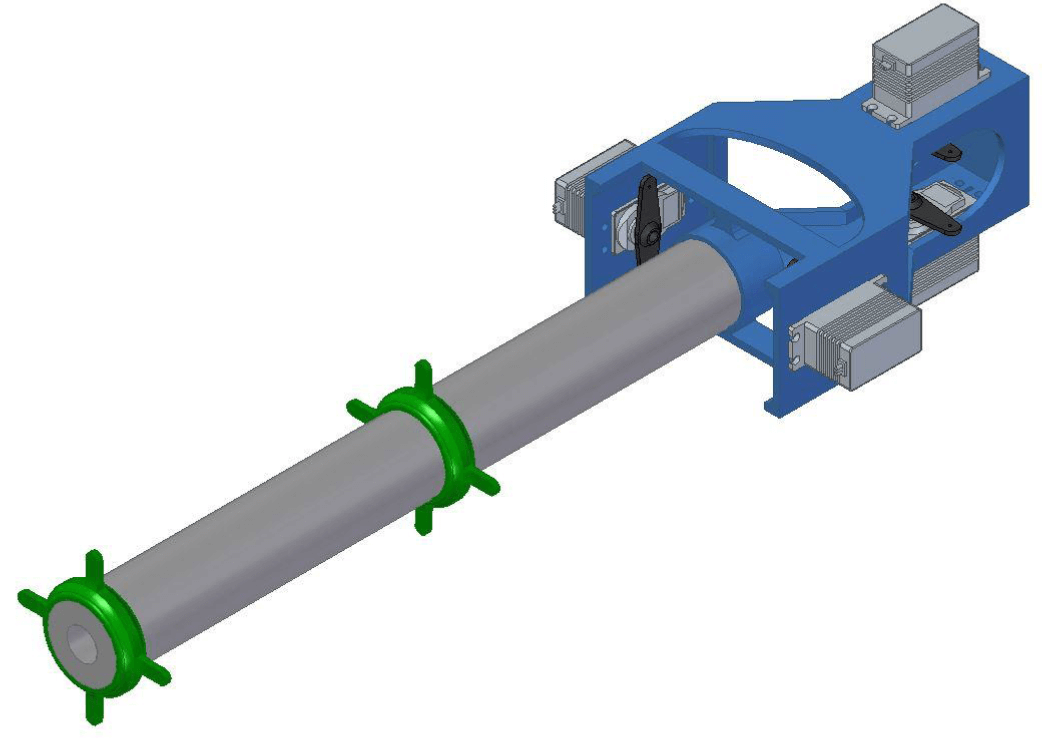
\includegraphics[width=0.75\textwidth]{images/initialConcept.png}
\captionof{figure}{Initial concept for the base of the robot, to house the servos and the arm.}
\label{figure:initialConcept}
\end{center}

At this point, the linkages to connect the arm to the servo cables were assumed to be circular discs with tabs for attaching the cables, sitting at the midpoint and tip of the arm to provide two degrees of freedom at each. This structure was then 3D printed at its initial dimensions in order to gain an insight into appropriate sizing and shape. The first issue was the physical finish of the printed part from the extrusion type 3D printer. Due to the design being a single structure with overhanging elements, a support structure was necessary to prevent collapse of the material during printing. When removing this excess material, abrasive edges were still present, making fittings such as the mounting bolts of the servos more difficult and scratching the foam when locating it within the holder, while also resulting in a generally unprofessional appearance. As such, it was decided to ensure future designs do not require support material during printing. 

When the servos were mounted to the base, the structure appeared unnecessarily large, where the makeshift wire reached the linkages without any points of near-intersection. Furthermore, due to the wide gap between the two horizontally configured servos, potential issues were discovered with stabilising the device through holding and manoeuvring it. Turning the device about the axis of the arm whilst these servos are particularly distant gives a much larger angular momentum than if they were close, making it more difficult for the user to turn the device in such a manner, as well as slowing it once started. Therefore, for any subsequent designs where the servos are in a twin-pair opposing configuration, the distance between the horizontal servos was to be minimised.

At this point, an alternative design was also considered, with the intention of minimising the distance of the servos from the user, requiring less moment force to hold. This design focused on being as compact as possible, and in such a manner that it could be printed in one piece without the difficulties associated with the first print. This concept thus took on a `cubic' shape, as depicted in Figure \ref{figure:cubicConcept}.

\begin{center}
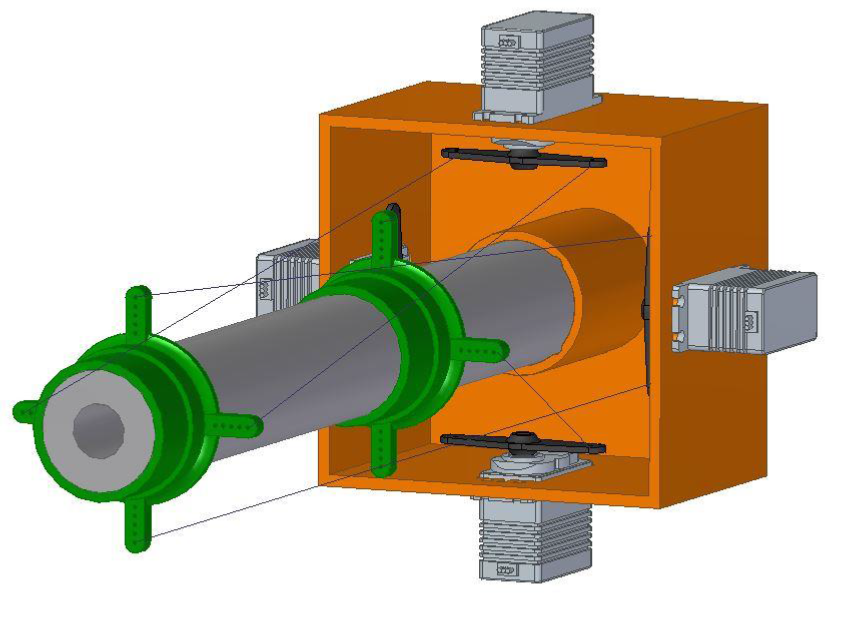
\includegraphics[width=0.75\textwidth]{images/cubicConcept.png}
\captionof{figure}{Cubic concept for the base of the robot, with the intention of being compact in length.}
\label{figure:cubicConcept}
\end{center}

In conjunction with the formation of this concept, the earlier prototype from Figure \ref{figure:initialConcept} was assembled using the generic servo arms and some spare wire to drive a pair of printed rings acting as the linkages on the arm. The servos were then connected to an Arduino UNO (coverd in more detail in SECTION XXXXX) in order to issue simple positional commands to test the motion of the arm. This revealed a few traits which warranted further design changes. The most notable was the way in which the servos were connected to the linkages; whilst the `direct line' approach as shown in both of the early concepts had the advantage of being virtually frictionless, motion response issues were found as a result. 

When a servo actuates, the response direction of the arm is not constant with increasing servo motion. That is, the arm initially moves in the direction along the connecting cable, and as the servo moves further, so does the starting position of the cable, changing the direction of motion of the arm. This response is made more unpredictable by the fact that the linkage in question could be in different starting positions depending on the angles of the other servos. Hence the actuation of a single servo is not constrained to an arm response in a single degree of freedom. This was envisioned to cause added complexity further down the design and control process, in that it would be much more logical and easier to account for if the cables were connected in such a manner that the actuation of a single servo could be ensured to result in motion in only one degree of freedom.

Other problems were also identified with the early implementations of linkages. Firstly, as the linkages were pulled in one direction and the arm deflected in response, gaps appeared between the arm and the linkage, causing the linkage to shift its position somewhat on the arm. Hence, the linkages were re-designed to be much longer axially, so that they interact with a larger portion of the arm so that there are no full gaps between the linkage and arm. Also, wrapping the cable around the tabs of the linkages was found to be a non-suitable solution, as they constantly came unravelled and lost tension almost instantaneously. Therefore, a series of holes along the tabs were to be used to interweave the wire between, creating a stronger grip through friction before fastening them through other means. This design transition of the linkages is illustrated in Figure XXXXX.

INSERT FIGURE OF EARLY DESIGN OF `FLAT LIKE' LINKAGE AND THE CURRENT DESIGN OF THE LONGER LINKAGE WITH MORE HOLES ETC AND THE BOLT HOLES XXXXXXXX

ELABORATE ON THE DESIGN OF THE LINKAGE A LITTLE BIT AND HOW THE CABLES ARE FIXED IN PLACE HERE OR AT END OF CABLE ROUTING SECTION XXXXX

\subsubsection{Cable Routing}
In order to limit the motion of one servo to arm movement in one degree of freedom, it was necessary to redesign the base structure in a manner that routed the cables to run parallel to the arm to the connection at the linkage. In order to have sufficient space to route the cables, it was decided that the staggered twin-pair servo arrangement would be better suited, allowing the servos to be positioned alternatively such that less extreme angle changes of the cables would be required. This can be accomplished by positioning two of the servos as close together as possible to pre-align the cable with the linkages to a degree, which would not be possible with a cubic arrangement. Of course, the design was then arranged in two halves, so that it may be 3D printed without any overhanging elements and need for support material. As a result, the centralised tube holder (to locate the base of the arm) was also a separate part that is located in a groove between the two halves of the base when they are secured together by four threaded rods and bolts. This arrangement is illustrated in Figure \ref{figure:halvesConcept}.

\begin{center}
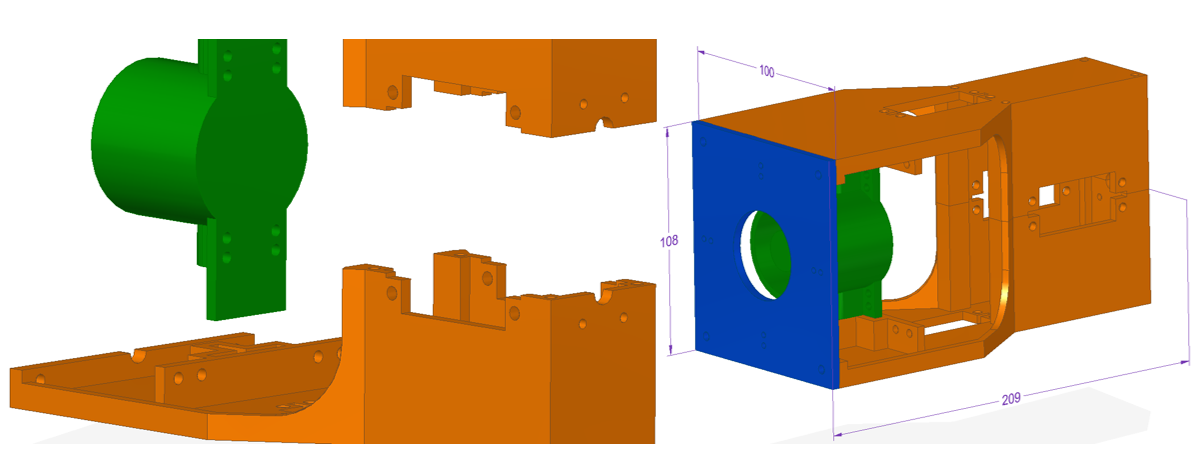
\includegraphics[width=0.75\textwidth]{images/halvesConcept.png}
\captionof{figure}{Identical halves for the base structure, with a separate centralised part to locate the arm.}
\label{figure:halvesConcept}
\end{center}

In this arrangement, the two rear servos are positioned close together while the front servos are further apart, creating space to run the cables of the rear servos between the front two without intersecting. A series of guidance holes are then put in place so that the cables can run parallel to the plane of their corresponding servo arms and tangentially to their starting position. These holes were positioned in the body of the tube holder itself and the housing groove on each half of the base used to locate it. Multiple holes were added so that different radius servo horns could be fitted if desired. In order to shift the direction of the cables one more time so that they run parallel to the axis of the arm, a simple square faceplate was to be fitted to the front of the base (not shown in Figure XXX). This just comprises a central hole for the arm to run through, and four smaller holes to each locate a pair of cables, aligned with the holes on the tabs of the linkages when the arm is in its neutral (straight) position.

As the cables change directions sharply at distinct points, namely the guidance holes, a reaction force will be felt at the contact point on the circumference of the holes. This force will increase linearly with the tension of the cables, which must be sufficient enough to stabilise the arm and manipulate it during servo actuation. hence wear of the cable on the rim of the hole was a concern, as this would cause added resistance to motion or, in the worst case, shear through the material so the cable is no longer routed. This was an issue apparent on the Mark I design in \cite{GreggSmithDesign}, and had to be addressed with extra attachments and rings to strengthen it against further breakages. As such, an ultra low friction cable was chosen from the offset, using a high-strength fishing wire (APPENDIX XXXXX). This exhibited no signs of wear during the phase of prototype testing, even when deliberately over-tensioned. Therefore no extra support fixtures were used and the cable ran freely over the PLA material of the base. With this, the dimensions were tweaked to move the front two servos closer together and to the rear servos, making the design more compact, and the dimensions were selected for the final design of the base, which overall were 209 x 100 x 108mm as illustrated in Figure \ref{figure:baseShape}.


\begin{center}
\includegraphics[width=0.75\textwidth]{images/baseShape.png}
\captionof{figure}{Overall shape and dimensions of base structure.}
\label{figure:baseShape}
\end{center}



\subsubsection{Pulleys}
With the design for the base structure in place, final parts were 3D printed and assembled to give the underlying foundation of the device so that the robot motion could be tested at the real base dimensions and servo locations etcetera. When setting the servos to a range of positions whilst moving the device to different orientations, issues were found with the way in which the servo horn drives the cables. Initially, the servos were fitted with the supplied standard two-sided servo horn (arm) with an overall diameter (furthest hole from the centre on one side to the other) of 50mm, as shown in Figure \ref{figure:servoArmChange}. The cable was connected by interweaving it between the holes on the arm, giving a friction grip, and knotting the loose end so it cannot pass through the hole. However, it proved a limited option of driving the cables in terms of available motion. At small servo movements from the starting position, a large response of the arm takes place due to the servo horn being perpendicular to the cable. However, at similar servo movements at higher angles, much smaller responses of the arm are observed. This is due to the cable being at an angle to the servo horn in relation to the perpendicular starting position, thus servo motion does not `pull' the cable as much. This effect is illustrated in Figure \ref{figure:servoArmChange}.


\begin{center}
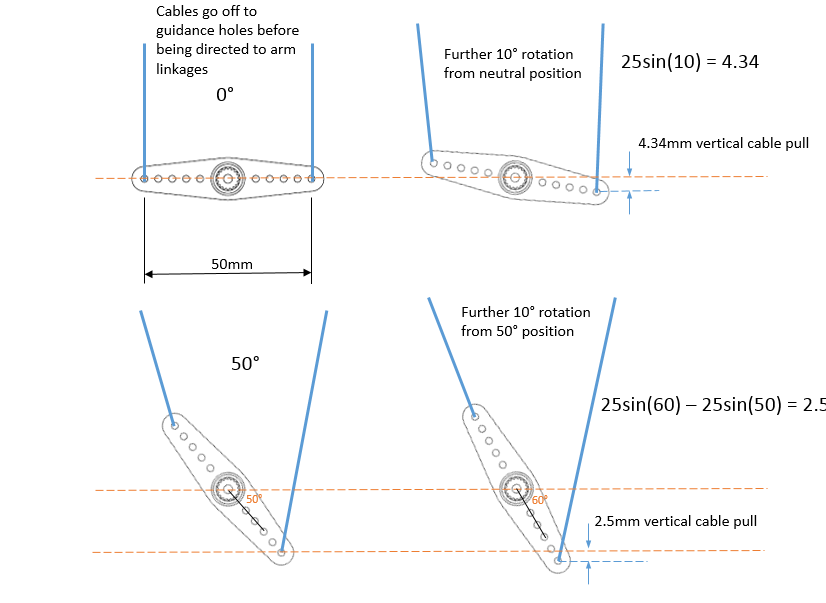
\includegraphics[width=0.8\textwidth]{images/servoArmChange.png}
\captionof{figure}{Vertical cable displacement (`pull') at a constant servo increment of 10 degrees, compared at different starting positions. Note that the horizontal cable displacement is ignored for simplicity as it has minimal effect on the pulling of the linkages.}
\label{figure:servoArmChange}
\end{center}

This effectively limits the potential range of motion of the arm in that only small responses can be achieved when the servos are already at a high position. On top of this, the image also shows that the angles of the cables going into the first set of guidance holes will also change with servo motion. The general effect of this servo horn type is a non-constant, and limited, arm response to servo actuation. As such, the arm motion can appear jerked and bumpy. In order to resolve this problem, it is necessary to employ a circular driving mechanism on the cables, so that the amount of pull is constant for a set servo increment, no matter what the starting position of the servo, this effect is illustrated in Figure \ref{figure:pulleyChange}.
 
\begin{center}
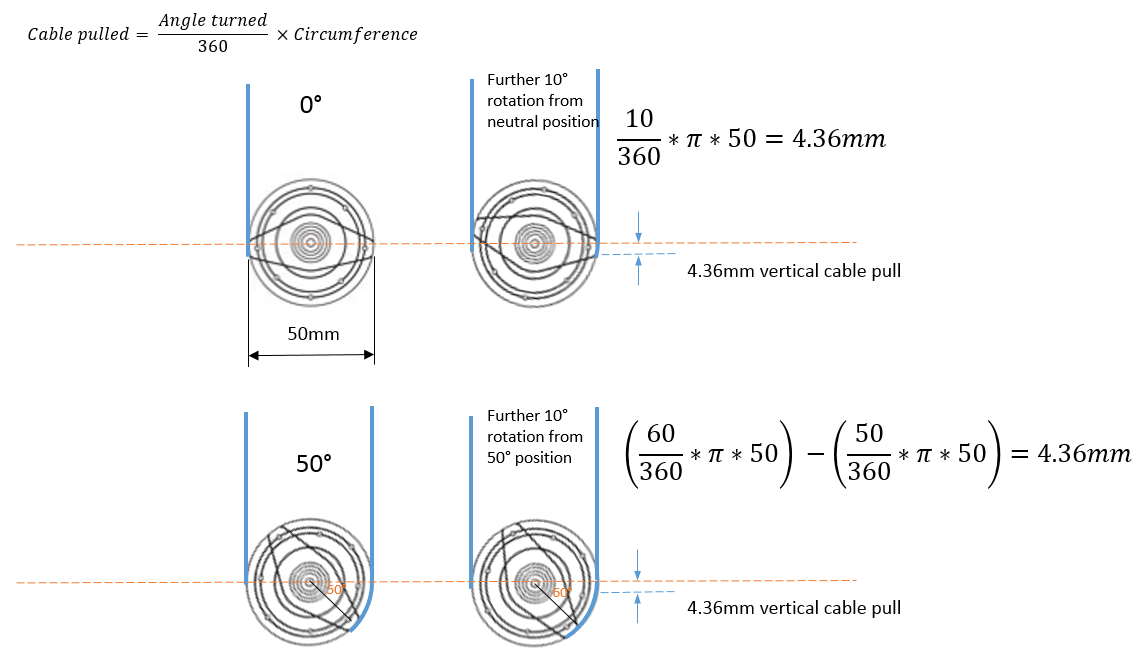
\includegraphics[width=0.8\textwidth]{images/pulleyChange.png}
\captionof{figure}{Vertical cable displacement (`pull') at a constant servo increment of 10 degrees using a circular attachment, compared at different starting positions. Assumed the cable is wrapped around the pulley before starting so unravels on side opposite to tension.}
\label{figure:pulleyChange}
\end{center}
 

As the image depicts, the cables also remain at a constant angle going off to the first set of guidance holes. This circular approach leads to generally smoother motion of the arm, a more constant torque requirement, and an improved maximum range of motion. As such, pulleys were designed to be fitted to the servos. The servos were also supplied with a circular horn of about 45mm in diameter, so this was to be used as the centre of the pulley to attach to the servo, and the diameter was to be stepped out to 50mm so the cables could run parallel to each other, tangentially to the pulley, and straight through the existing guidance holes. The holes in the circular horn were used to pass one continuous cable through, so the free cable length is equal on each side to be used for driving the linkages. The pulley then, was designed at two separate parts to be glued together, with a groove for the circular horn to be glued into. A small slot between the two halves could then be used to pass both ends of the cable through, so that it exits straight into the pulley groove to be wrapped around. This design is illustrated in Figure \ref{figure:pulleyDesign}.

\begin{center}
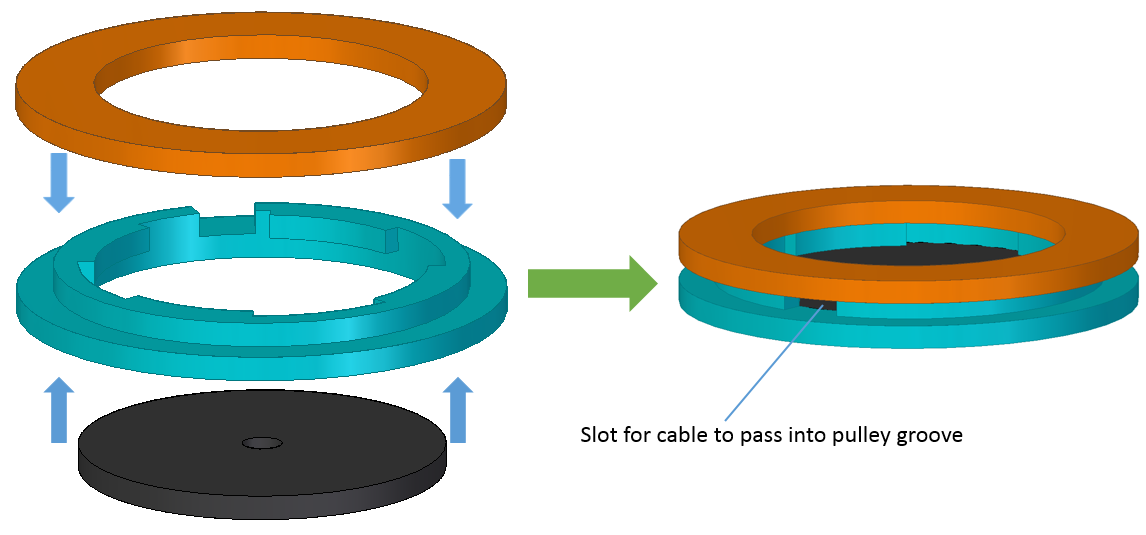
\includegraphics[width=0.8\textwidth]{images/pulleyDesign.png}
\captionof{figure}{Three separate parts that make up the pulley design, including the supplied circular servo arm to interweave the cable into to constrain it.}
\label{figure:pulleyDesign}
\end{center}



\subsubsection{Final Design}

Once the pulleys were constructed and fitted to the servomotors, the motion of the arm was much improved in terms of smoothness and maximum range. However, when the arm was moved from its neutral position, an issue was identified with its stability. Of course, the cables that were currently pulling the arm were taught, although the opposing cables had become particularly slack. The implication of this was that the opposing cables offered no resistance against further arm motion in the direction it was being pulled. This issue was exacerbated when the device was held parallel to the ground, as the arm appeared to `sag' towards the ground when pulled downwards, due to the added force of gravity and no tension in the upper cables to resist this motion. This comes about as a result of the path of the cable on the non-taught side of the arm. As the arm deflects, the amount of cable let out by the pulley is greater than the increase in length required to follow the arm motion, hence the loss of tension. Specifically, this is a result of the cable being connected in discreet straight-line segments to the linkages, whereas the arm itself curves when deflected. The effects of this problem can be reduced by adding more linkages to the arm, purely to guide the cable and increase the total distance the cable covers during arm deflection. This problem, along with the solution, is illustrated in Figure \ref{figure:slackReduction}.


\begin{center}
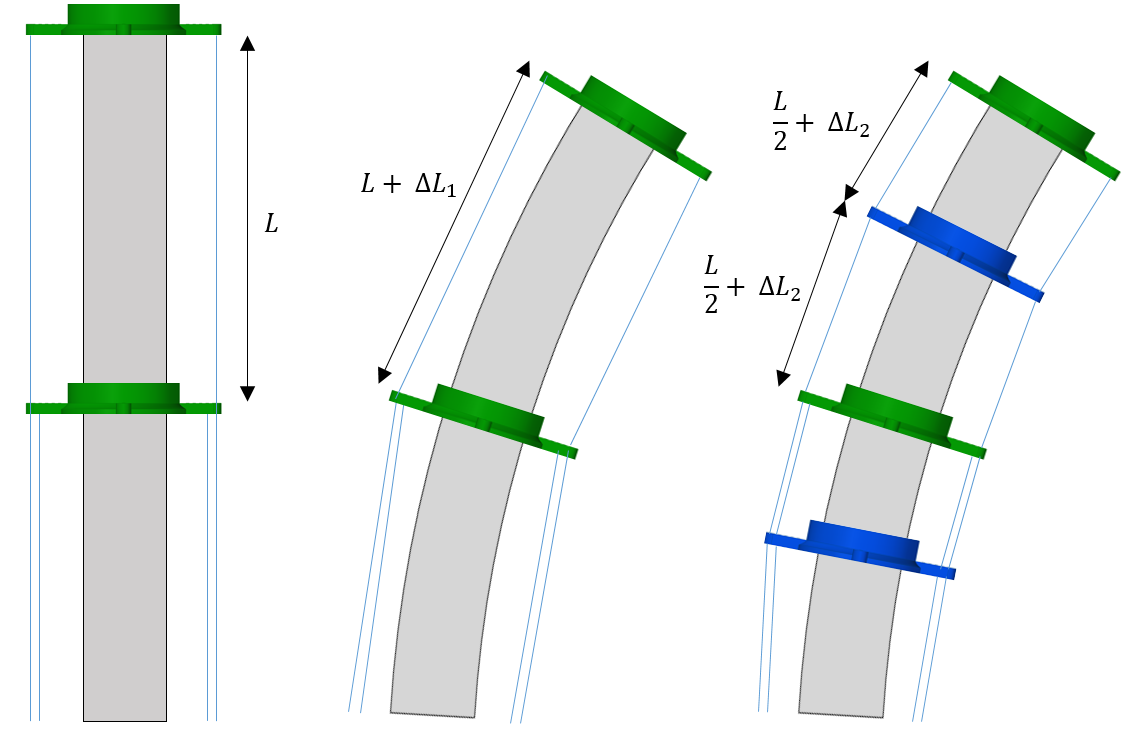
\includegraphics[width=0.8\textwidth]{images/slackReduction.png}
\captionof{figure}{Varying length of the cable on the side opposite the pulling (taught) cable during arm deflection. Adding guidance linkages increases the cable extension during deflection (assuming constant arm curvature), reducing excess cable released from the pulley. Left: neutral position, Centre: deflection without guide linkages, Right: deflection with two added guide linkages.}
\label{figure:slackReduction}
\end{center}

As more guidance linkages are added to the arm, the distance the cable must travel from the central linkage to the tip linkage during deflection is increased. This is because the guidance linkages maintain the cable at a set perpendicular distance away from the surface of the arm as it passes through their guide holes. Without this, as shown in the central image of Figure \ref{figure:slackReduction}, the cable goes from the mid-point to the tip of the arm in a straight line, coming much closer to the surface of the arm. Hence, this length comparison can be expressed as:



\begin{equation}\label{equation:guidanceLength}
2(\frac{L}{2} + \Delta L_{2}) > L + \Delta L_{1}
\end{equation}

Therefore, there is a smaller difference between the amount of cable let out by the pulley and the extra amount taken up to follow the deflection of the arm. This means that there is less loss of tension, and thus more stability of the arm and resistance to further motion in the direction of the deflection. As such, two guidance linkages were added to the arm, at the mid-points between the two sections of the arm. A simple mounting surface for the magnetic end effector was then used as a linkage cap and glued to the tip linkage, giving a total arm length from base to tip of XXXXXXX. This completed the physical design of the mechanical aspects of the robot, including the base, the arm and the cable driving mechanism, as illustrated in Figure \ref{figure:rendering}.

\begin{center}
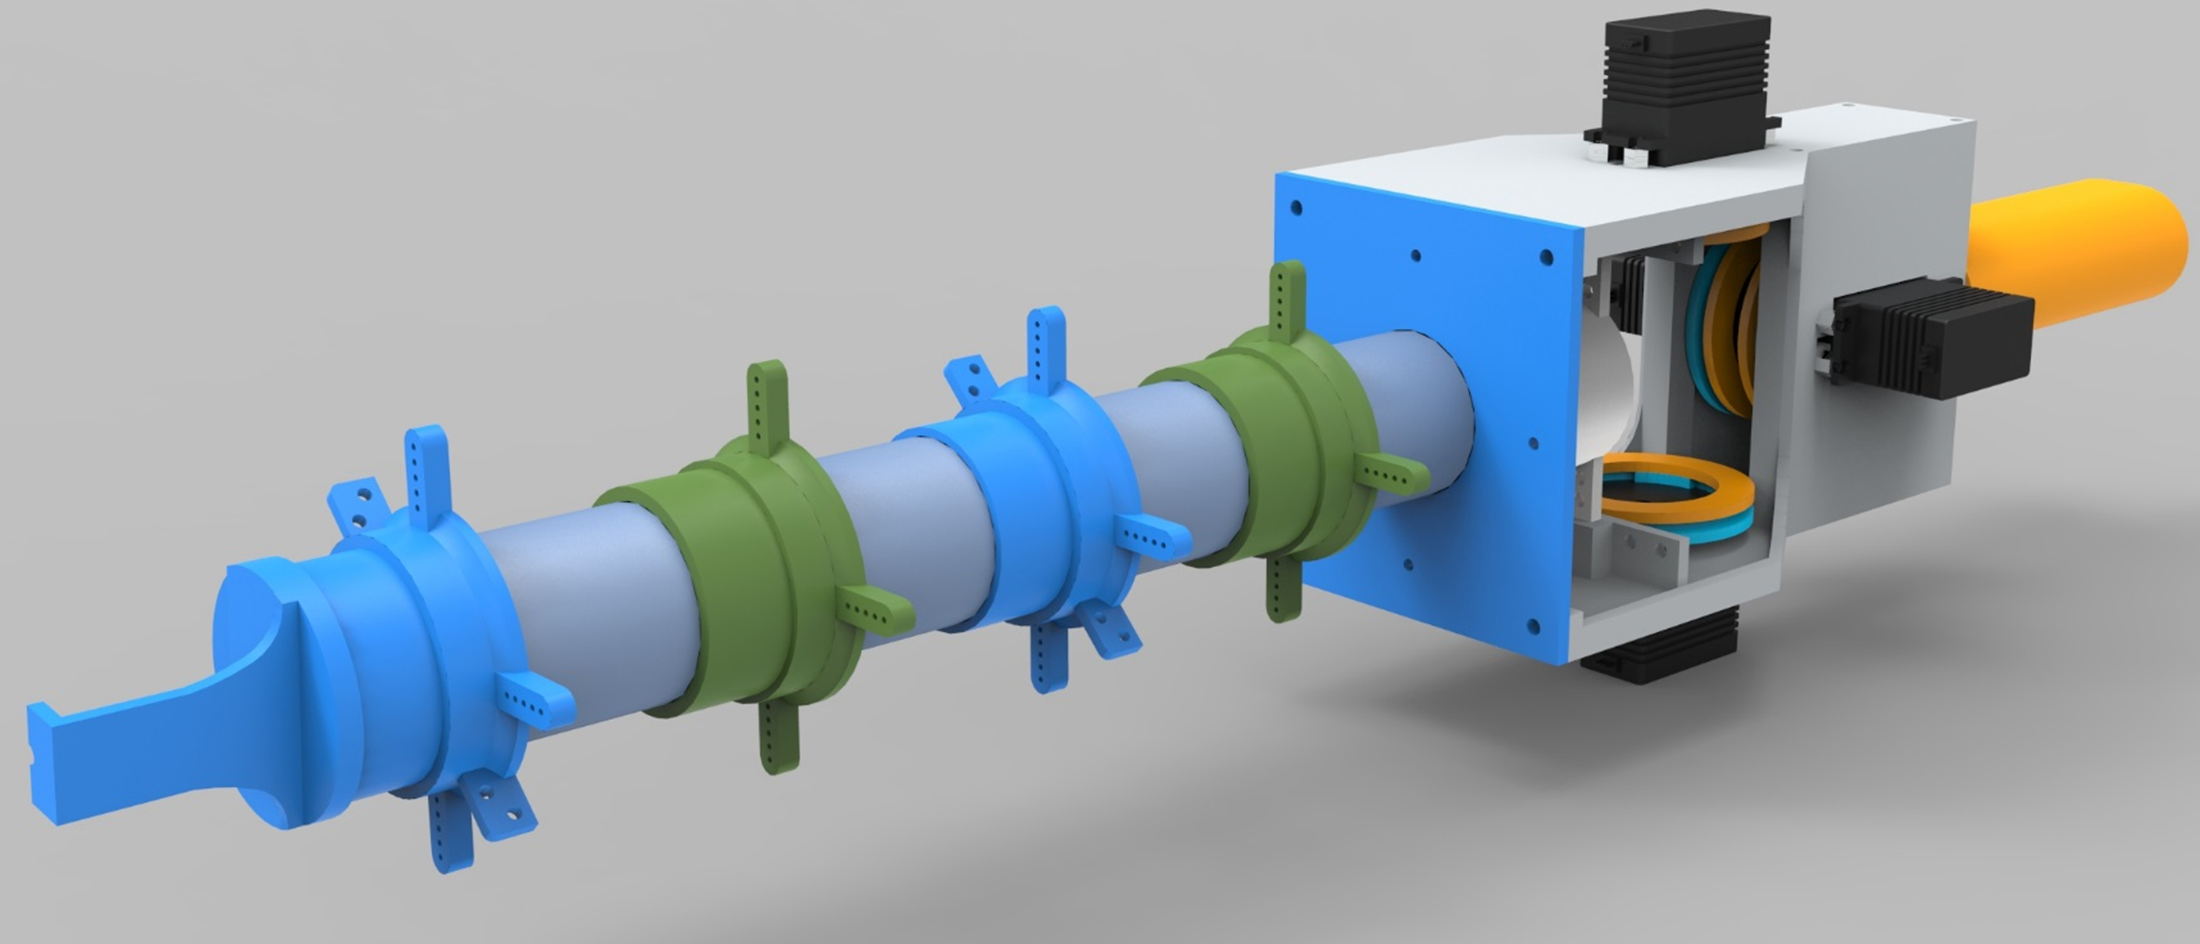
\includegraphics[width=\textwidth]{images/rendering.png}
\captionof{figure}{Rendering of the design of the base and arm of the robot}
\label{figure:rendering}
\end{center}

\subsubsection{Ancillaries}
Due to the nature of the project, it was unrealistic within the scope to also design a novel end effector for the robot. Therefore, it was decided to simply use an electromagnet of some form, and design the physical aspect of manipulating objects around magnetic interaction, i.e metallic strips enabling them to be picked up. The chosen option for employing an electromagnet was to use the copper coil and metallic cylinder from the central core of a small solenoid (APPENDIX XXXXX). This solenoid was disassembled to obtain just the necessary components for the electromagnet, and was then fitted to the surface mount at the tip of the arm. A small groove in the metallic cylinder of the solenoid slotted onto a similar sized semi-circle bore at the front face of the surface mount (visible in Figure \ref{figure:rendering}, to prevent the cylinder from moving axially when the current flows through the coil and magnetic force is induced. The exposed end of this cylinder is then, in essence, the `grabbing' part of the robot, as it is magnetised and put in contact with metallic targets.

PERHAPS IMAGE OF THE DISASSEMBLED ELECTROMAGNET HERE? XXXXXXXXX

In order to use the robot in an intuitive, user friendly manner, it was decided to modify a conventional handheld power tool. This must be ergonomic in terms of handling the robot, while also providing a trigger or switch so that the user may send signals to the device to instigate a required action. As a result, a standard outdoor grass strimmer was procured (APPENDIX XXX) and modified to remove everything but its base (handle, trigger and shaft). A sleeve was then designed to connect the robot with this base. This was a near-cylindrical cross-section tube which was simply bolted to the bases of the robot and the strimmer, completing the handheld component of the device.


\pagebreak
\subsection{Controlling The Device}

In order to properly control the device, it was necessary to implement a microcontroller to interface between the actual control program, and the robot. As such, an Arduino UNO R3 (APPENDIX XXXXX) was selected to sit between the PC that runs the program and the various electrical components of the robot (the servomotors and electromagnet). The servomotors themselves (APPENDIX XXXX) require a 6V power source, thus two 4 x AA (1.5V) battery boxes were connected in series. The position of each servo is determined by the value from the corresponding PWM (Pulse Width Modulation) pin on the Arduino. 

The electromagnet requires 9V for generating adequate magnetic force. So in order to safely control this, enabling the magnet to be switched on and off as required, it was necessary to use an Arduino Motor Shield (APPENDIX XXX). This allows a 9V battery to be connected via the $V_{in}$ and $Gnd$ terminals, with the output power and ground wires connecting to the electromagnet. A pin on the Arduino is then designated for turning this output power on and off. There are then two options for controlling this magnet, by having the trigger of the strimmer base hooked up directly on the power wire to the electromagnet, or by having it connected to a pin on the Arduino that can respond by setting the pin that controls the power output. The former option would result in the magnet being on whenever the trigger is pressed, whereas the latter option allows for much more options. These include responding in other manners from the trigger press, counting the number of trigger presses and only turning on the magnet if the device is `in range', saving battery. Hence, the second option was chosen. A schematic of this set-up is illustrated in Figure \ref{figure:schematic}.


\begin{center}
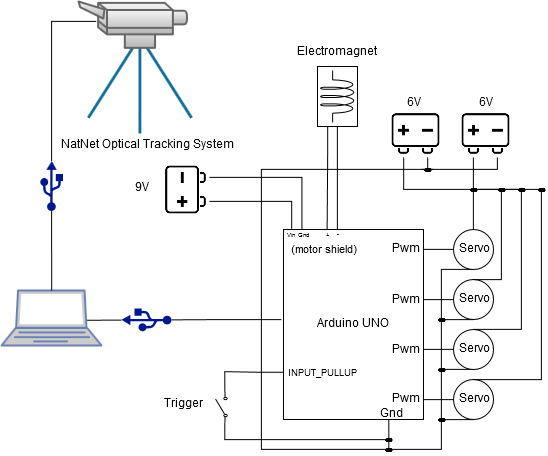
\includegraphics[width=0.95\textwidth]{images/newSchematic.png}
\captionof{figure}{Schematic showing how the controlling equipment interfaces with the pc and the robot components.}
\label{figure:schematic}
\end{center}

Of course, the optical tracking system also interfaces with the controlling PC in order to receive the necessary tracking information. This is shown in the schematic for completeness. To send commands and receive information from the Arduino, a serial connection is set up in C\# using the SerialPort class. Once a connection is established, commands are sent in the form of a buffer of bytes, which are interpreted and responded to by the Arduino sketch. These commands include setting the position of a servomotor and turning on the power for the electromagnet; an example of this process with the program command and Arduino response is shown in Appendix XXXXXX.

All of the components were then assembled in place using an Arduino Proto-Shield and a mini breadboard. This was set up in a manner that allowed the battery packs and servomotors to be easily interchanged as required, whereas the control circuitry was fixed in place, as illustrated in Figure XXXXXX.

INSERT PICTURE OF NEATLY ASSEMBLED CONTROL CIRCUITRY ON THE ROBOT WITH THE PROTOSHIELD AND MINI BREADBOARD ETC XXXXXXXXXXXX

The finalised construction of the new handheld robotic device is thus illustrated in XXXXXXX.

INSERT FULL PICTURE OF THE ROBOT AS A WHOLE, MAYBE WITH CLOSE UPS OF THE BATTERIES, CIRCUITRY, AND END EFFECTOR ETC AS SIDE IMAGES IN A COLLAGE XXXXXXXXXXXXXX

\pagebreak
\section{Developed Program}

\subsection{Interfacing With NatNet Optical Tracking System}
\label{section:natnet}
In order to determine where in three dimensional space the robot is, as well as the relative distances between itself and other points, it is necessary to track physical objects. This was achieved using a single optical tracking device, the OptiTrack V120 Duo \cite{OptiTrackSite}. The device features two cameras in order to provide depth perception, and works as a stand-alone device unlike the syncing of several distinct cameras as used in \cite{GreggSmithDesign} and \cite{GreggSmithFeedback}. The accompanying software library however, the `NatNet SDK', as well as the actual tracking software, `OptiTrack Motive', are the same. This library was provided to run in a .NET framework environment, hence the decision to use C\# as the primary development language.

The device recognises the supplied retro-reflective markers, and is able to provide six degrees of freedom tracking. It is important to not that the coordinate system used by the software (the global axes) originates from the positioning of the Duo tracking device itself, as illustrated in Figure \ref{figure:duoAxes}. Single markers can be identified in terms of their X, Y and Z positions, and can be grouped together to form `rigid bodies`. These bodies, requiring a minimum of three markers, have a designated `centre' that can be used to refer to the position of the body as a whole, and provide a pivot about which rotation can be expressed. The rotation is inherently given as a quaternion, which can be converted using built-in library functions to give euler angles in the forms of roll, pitch and yaw (rotations about the global X, Y and Z axes respectively).


\begin{center}
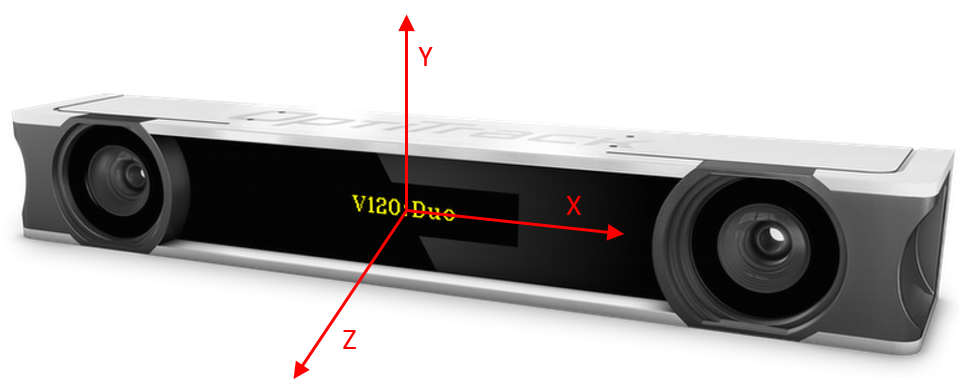
\includegraphics[width=0.8\textwidth]{images/duoAxes.png}
\captionof{figure}{Axes as used by the OptiTrack Motive software, these global axes originate from the centre of the device, image adapted from \cite{OptiTrackSite}}
\label{figure:duoAxes}
\end{center}

The rigid bodies must be configured within the Motive program, selecting which markers comprise them and giving them a name. Moreover, individual markers can also be identified as requiring to be tracked. Hence a rigid body will be configured for each of the base and the tip as a bare minimum. With the Motive program running in the background, the NatNet library can be used to extract tracking information from the program. This is done by identifying the program as a server application and connecting it with the local ip address. Once established, and the fundamental NatNet client object is instantiated, the event based data handling is started. This refers to the server application (Motive) triggering an event with a corresponding callback every time a new frame of motion capture data is ready, which is passed into the callback to be processed as desired. This frame of data contains all of the tracking information that Motive is set up to capture. For example, a list of all the rigid bodies, which takes the form of objects storing the name, positional values, rotation (quaternion) and a contained list of individual markers with their own information.

Therefore, rigid body objects can be set up to represent the robot base and tip which, every time a new frame is sent from the program via the callback function, can be updated so they represent the current tracking information. Similarly, other variables pertaining to these bodies, such as the relative distance between tip and base, can be set up and updated as part of the callback function once the rigid bodies themselves have been updated. As a more practical alternative, a separate thread can be set up so that, although a global variable representing the current frame of motion capture data is updated as soon as a new frame is ready, the rigid body objects or other relevant variables can be updated when desired (after a set time interval) by fetching information from the current frame of data object at any point. Of course, when doing so, it is important to put a read-lock on a shared object so that the frame can be read and data extracted safely without the event based thread updating any of the data mid-read.

Once the required tracking data has been extracted, it can then be manipulated to create relative target points to the base depending on the situation. These can then be used as inputs to the regression function in order to solve for the motor angles. The tracking data at certain points is also written to an XML file during the calibration procedure, as mentioned in SECTION XXXXX. 

\subsection{Kernel Regression Method}
Due to the nature of the design of the robot, particularly the flexible arm in which motion from one of the core arm linkages would affect the other, solving for the kinematics is highly non-trivial. The arm itself exhibits nonlinear characteristics when flexing, rendering established forms of kinematic modelling unsuitable. A nonlinear kinematics solution was provided for a single segment of a cable driven continous backbone in \cite{li2002}, demonstrating the complexity involved in just one section. Thus, an alternative approach was taken similar to that in \cite{GreggSmithDesign}, which is unsurprising due to the parallels between the two designs; the arms are of different size and material but are both non-linear in nature and composed of multiple sections. The solution, as covered in \cite{GreggSmithDesign} and again in more detail in \cite{GreggSmithPhd} is to use a kernel regression method.

The method specifically is known as the Nadayara-Watson kernel regression \cite{nadaraya1964}. It operates on the principle of using known data points to interpolate between, and yield a solution from an input that is not necessarily present in the known data. The function itself is given below in \eqref{nadaraya}.

\begin{equation}\label{nadaraya}
\bar{y}(\bar{x}) = \frac{\sum_{i=1}^{n}y_{i}K(\frac{x - x_{i}}{\alpha})}{\sum_{i=1}^{n}K(\frac{x - x_{i}}{\alpha})}
\end{equation}

Where $K$ represents a kernel function, $\alpha$ the bandwidth, $x$ the input and $y_{i}$ and $x_{i}$ the values of the stored data for the output and input values respectively. The bandwidth, as expected, will have a large effect on the output of the function. This could best be represented by a plot of the output of the function for a range of inputs at a given bandwidth. Of course, due to the number of dimensions in this case (three for the positional vector and four for the motor angles), it is not easy to give a visual representation, hence a 2D example is given in Figure XXXX for the non-linear  function $cos(\frac{x}{10}) + (\frac{x}{60})^2$. 

FIGURE ILLUSTRATING THIS EFFECT, USING 2D GRAPH AS IN AUSTIN THESIS???XXXXX

As shown in the figure, for a smoother plot, covering the areas not covered by the stored points at the expense of accuracy compared to the actual stored point values, a higher bandwidth would be expected. However, a lower bandwidth would result in a rougher, more sporadic plot, with the effect of intersecting all of the stored points exactly. As shown by the two plots, adding more samples acts to smoothen out this latter case, giving a smoother plot whilst improving the accuracy compared to the actual values. An optimal bandwidth would of course produce a minimal error for compared to the actual values of the points the sampling does not cover. High degrees of non-linearity are typically characterised by a comparatively lower optimum bandwidth.

Given the way this regression works, all of the recorded points will have an effect on the outcome. However, it is desirable for the recorded points close to the input point to have a greater effect on the result than those further away, meaning smaller values of $x - x_{i}$ will make less of a contribution to the $\bar{y}$ value. Therefore, to cater to this requirement, the chosen kernel function, $K$, was a Gaussian kernel function, as given in \eqref{equation:Gaussian}, due to its bell-curve shape and how input values close to zero have a larger output effect.

\begin{equation}\label{equation:Gaussian}
K(u) = \frac{1}{\sqrt{2\pi}}e^{-\frac{1}{2}u^2}
\end{equation}

With the given kernel regression function, the corresponding output values could be found for various different types of input values. The function itself does not depend on the number of dimensions, and hence the $y$ and $x$ values can be of any vector size, as long as they are consistent and each input type value is paired with a corresponding output type value within the recorded data. This is because the value used as an argument for the kernel function depends on an absolute difference between the two vectors, which will be a single number regardless of their size, giving an overall output value of the correct number of dimensions. In the given scenario of the robot and the data that is recorded, the matching output types are shown for input types in Table \ref{table:regressionOutputs}.

\begin{center}
\captionof{table}{List of corresponding output vector types for a given input vector}
\label{table:regressionOutputs}
\begin{tabularx}{0.66\textwidth}{ | >{\centering\arraybackslash}p{12em} |>{\centering\arraybackslash}X|} 
\hline
Input vector & Output vector\\
\hline
motor angles $\bar{m}$ & relative tip position $\bar{p}$ \\
relative tip position $\bar{p}$ & motor angles $\bar{m}$ \\
relative tip orientation $\hat{d}$ & motor angles $\bar{m}$ \\
$\bar{p}$ and $\hat{d}$ & motor angles $\bar{m}$\\
\hline
\end{tabularx}
\end{center}

This list of input and output types is similar to that observed for the table input/outputs given in \cite{GreggSmithDesign}, as expected due to the similar methods. However, in this instance, only the tip position is returned when given the motor angles, as this project is of much smaller time scale and the orientation is less critical to the required steps. Once the regression method itself was planned and tested with some sample data, it was necessary to acquire real calibration data in order for it to work and to fine tune the bandwidth appropriately.


\subsubsection{Calibration Procedure}
DON'T FORGET IMAGES OF ROBOT IN CLAMP FOR VISUALIZATION, SHOWING IT IN TWO DIFFERENT POSITIONS TO SHOW DIFFERENT DATA POINTS BEING LOGGED XXXXX

The procedure for obtaining the calibration data involves sending a range of different motor angle configurations to the servomotors, and recording the resulting tracking information (relative tip-to-base position and orientation). Each data point then comprised all of these values, and was written to disk for re-use in the future when using the regression function. When recording the data, it is imperative that the robot base remains stationary, so each data point is consistent with the same base position and orientation. As mentioned in Section INTERFACING WITH TRACKING XXXXX, the base is said to have zero orientation about any of the global axes if it is in the orientation that it was when it was first initialised in the Motive software (as a rigid body). Hence the base was secured in a vice and then initialised in Motive (along with the tip) before beginning the procedure. This set up is illustrated in Figure XXXXX, with the identification of the base and tip in the Motive software shown in Figure XXXXX. The physical orientation of the base during calibration is of little importance (as long as all points are always visible to the tracking device), as the targets will be relative to the base and converted to its orientation anyway, as covered in more detail in Section XXXX.

INSERT IMAGES XXXXXXX


The calibration sampling is then performed at a chosen resolution (number of degrees interval) by stepping through the full range of motion for one servo for each step of a `parent' servo. Thus if each servo (apart from the last in line) has a `child` servo, the motions are performed recursively, with the servo stepping once, then its child covering the full range, with its grandchild then covering the full range for each step of its child and so on. Hence a recursive function was written as shown in Figure XXXXXX INSERT CODE OF CALIBRATE FUNCTION AND PUT IN BODY OR APPENDIX?? XXXXX. The function is written such that after each step of a motor, its child motor then covers the range of motion in the opposite direction to its previous one. This is to reduce the number of times a motor has to move all the way back to the start of its range before stepping again, making the motion smoother in general and reducing calibration time. 

INSERT CODE IMAGE OR PUT IN APPENDIX XXXXX	





\subsubsection{Calibration Results}
In order to find an appropriate bandwidth for the regression function, it was first necessary to obtain calibration data through sampling. Once enough data is available to perform the regression, the function can be tested against other sampled data, not covered in the initial calibration data, referred to as the `test data'. By comparing the output of the function for different bandwidth values against the values of the test data, an absolute positional error can be determined. 

FOLLOWING TWO PARAGRAPHS SHOULD REALLY BE IN THE CALIBRATION PROCEDURE SECTION NOT THE RESULTS XXXXXX

The state-space of the arm was initially sampled at a chosen resolution of five points over a total range of 60\degree per servo, giving a total sample number of $5^4 = 625$ calibration points. This gave a suitable range of motion, with an improvement of 20\degree over the device in \cite{GreggSmithDesign}. Higher ranges were initially used without any long term issues, although temporary deformation of the foam arm meant that the cables need to be re-tensioned, which was especially time consuming. A one second pause was issued after each calibration step to ensure the tip was steady before the position was logged. Hence this calibration took just over 10 minutes. Of course, higher accuracy could be obtained through more samples, with an increase in time, but this was kept short due to the fact that it needed to be repeated a lot with small design changes. Also, a meaningful increase in accuracy would require numerous extra sample points, quickly increasing the required time to well over an hour, which introduces other problems such as battery issues and gradual deformation. The surface covered by this calibration procedure is illustrated in the Figure XXXX, displaying alternate views to better represent the curved shape of the area covered, similar to a portion on a sphere.


MAYBE JUST SHOW THE TOP AND BOTTOM CALIBRATION SURFACE PLOT OR EVEN JUST TOP? XXXXXXXXX


\begin{center}
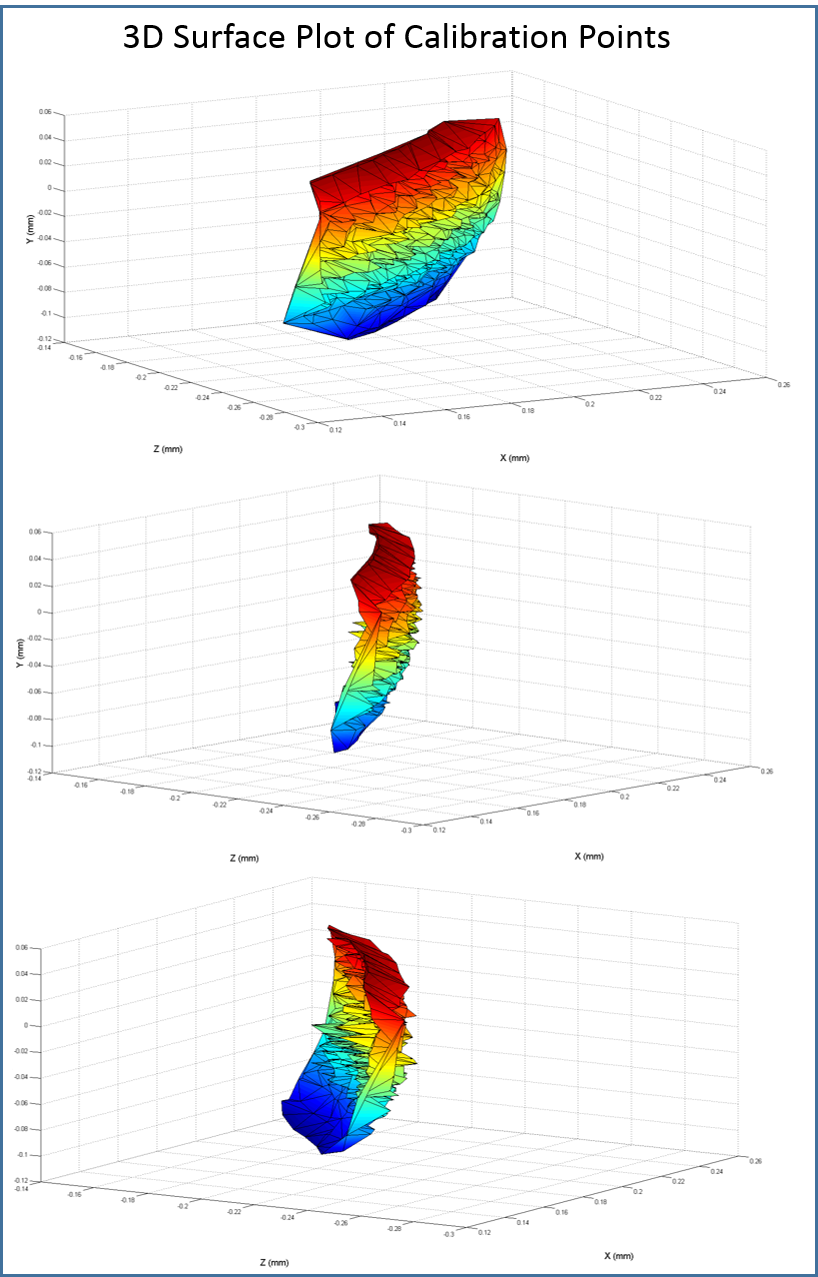
\includegraphics[width=0.9\textwidth]{images/surfacePlotTogether.png}
\captionof{figure}{Three alternate views of the surface plot for the 3D area covered by the calibration points, note the forward and backward spikes for when the arm took on an `S' shape, pulling the tip inwards somewhat.}
\label{figure:surfacePlot}
\end{center}


The number of test data points was considerably smaller, with the primary aim of just collecting data for motor angle vectors that were not covered in the initial sampling. Hence $3^4 = 81$ samples were obtained, with starting position and step selected to deliberately avoid any calibration samples. For the comparison between the function output and the test data, the motor angles were to be the input, thus comparing the output positional values with the recorded points for the same motor angles. This `forward' approach was used for two reasons. The first is because the errors could be compared in terms of millimetres in space, which is more meaningful than servo degrees. The other reason is due to the fact that a given 3D position could potentially be achieved (or very close to) by more than one configuration of servo angles, whereas there is only one matching position for a given angle configuration. The 3D points for the calibration and the test points are illustrated in Figure \ref{figure:calibrationTestPoints}. 


\begin{center}
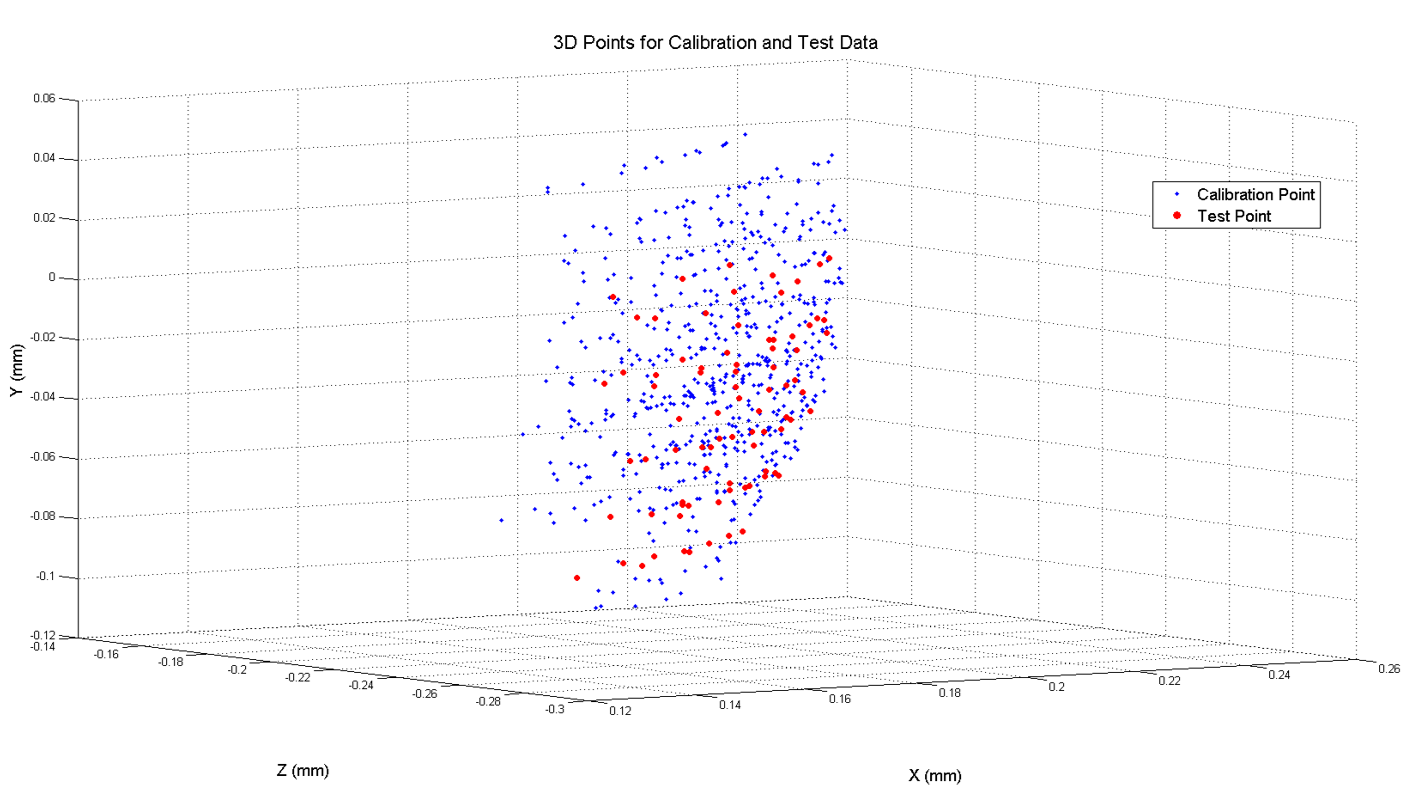
\includegraphics[width=0.95\textwidth]{images/calibrationTestPoints.png}
\captionof{figure}{Calibration and test points represented in 3D space, note that although some of the points in 3D space may intersect, the underlying servo angles will all be different.}
\label{figure:calibrationTestPoints}
\end{center}



Due to the nature of the kernel function, large differential values (the $x - x_{i}$ term) can cause issues. The input to the kernel function becomes larger when divided by the bandwidth (typically less than one), meaning when this value is squared, negated and made an exponent, a very small number is the result. This becomes particularly problematic when the value is so small that the number of bits required to represent it exceed those available in the `double' data type, giving a result of zero out of the Gaussian kernel function. This then can then cause the regression itself to fail as the denominator becomes zero, giving NaN values as output as opposed to any meaningful values. Due to the typically observed differences in degrees between the servo angles of the input and the sample points, this issue was present. As such, the value of servo angles need to be scaled so that the difference between any values is guaranteed to be in the range of $-1 < x - x_{i} < 1$. This is known as feature scaling, or min-max normalization \cite{mohamad2013}, and is shown in \eqref{featureScaling}, where $x^{\prime}$ is the new value after the original value, $x$, was scaled. This was performed for all servo angles during the regression function, and converted back after output to get results in degrees.

\begin{equation}\label{featureScaling}
x^{\prime} = \frac{x - x_{min}}{x_{max} - x_{min}}
\end{equation}

The function was thus used for each of the 81 angle configurations covered by the test data, giving a mean positional error (mm) between the output and test data values. This was then repeated for a range of bandwidth values and plotted to determine the most suitable value to minimise error, as illustrated in Figure \ref{figure:bandwidthPlot}.


\begin{center}
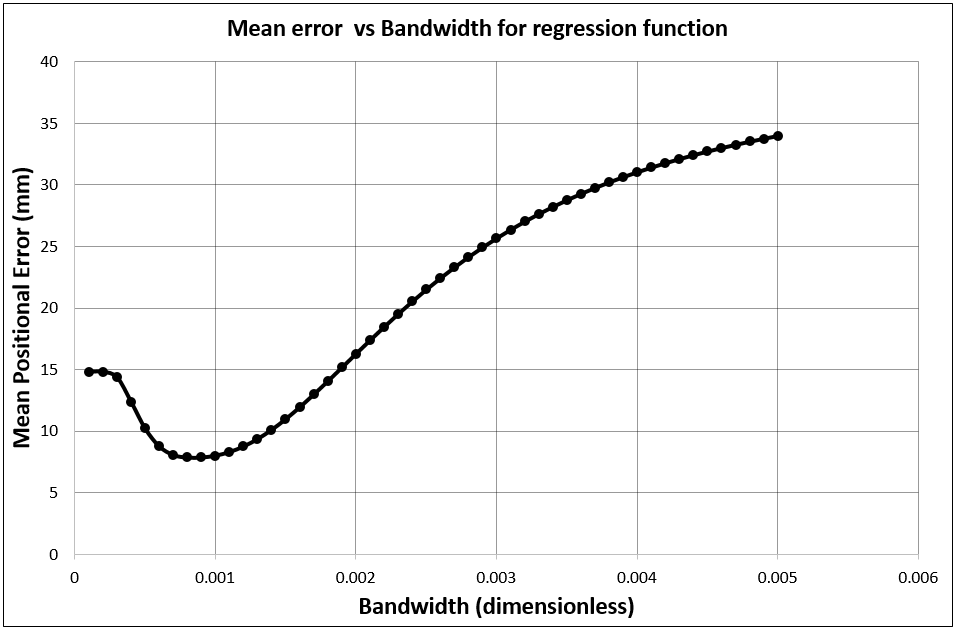
\includegraphics[width=0.9\textwidth]{images/bandwidthPlot.png}
\captionof{figure}{Mean positional error at various bandwidths for the output of the regression function compared with the corresponding real positional data}
\label{figure:bandwidthPlot}
\end{center}

AS SHOWN IN THE GRAPH, THE OPTIMAL BANDWIDTH IS AT ABOUT 0.0008, WHICH GIVES A MINIMAL ERROR OF ~8MM. THERE ARE A NUMBER OF REASONS WHY THIS ERROR IS NOT SMALLER THAN IT IS, SUCH AS THE FOAM DEFORMING SLIGHTLY AFTER EACH CALIBRATION PROCEDURE AND THE NUMBER OF SAMPLES NOT BEING PARTICULARLY HIGH. FURTHER DESIGN CHANGES TO MITIGATE THIS OUTSIDE OF THE SCOPE OF PROJECT, EXPECTED WITH LESS RIGID ARM ANYWAY, MITIGATION ACTION WAS TO NOT USE BLOCKS THAT WOULD BE SMALLER IN SIZE THAN THIS ERROR ETC ETC. XXXXXXXXXXX
Low bandwidth shows high non-linearity as expected due to arm material etc


CHANGE THIS TO SHOW THE OPTIMAL BANDWIDTH VALUE WHEN ACTUALLY USING THE FEATURE SCALING, NOT DIVIDING BY 10000? XXXXX

\pagebreak 
\subsection{Algorithm for Responding to Three-Dimensional State Targets}
Once the robot has been calibrated in such a way that there exists a suitable range of data points in which to perform the regression function, along with the selection of an appropriate bandwidth, the device may then be responsive to 3D state commands.
The process of responding to commands is fundamentally built on inputting a positional vector, an orientation vector or a combined vector into the regression function in order to ascertain the required motor angles. This input vector is of course in regard to the tip relative to the base, as is the corresponding calibration data. The resulting motor angle vector is then issued to the servomotors via the Arduino in a controlled manner. 

However, in order for this approach of obtaining servo angles from a given input to be useful in practice, it is first essential to determine the correct input to the regression function. This can depend on a variety of factors relating to the absolute 3D target point and its relation to the base of the robot, such as the current orientation of the base and the relative proximity of the target.

\subsubsection{Acquiring Target Position Relative to Orientation of Base}
The robot is fixed in place while the optical tracking software is configured to recognise the rigid bodies formed by the retro-reflective markers associated with the base and the tip, as covered in Section \ref{section:natnet} (just say 'is configured'?. At this point, the base is said to have zero orientation about any axis (as this was the point it was first initialised in). The calibration procedure is then of course undertaken while the robot is fixed in this position. Thus, the stored relative tip-to-base calibration data for different servo angle vectors is only valid for the robot in a zero orientation state compared to the starting position. Hence, in practice, when the base has changed orientation about any of the three axes inherent to the optical tracking device, a direct input for a relative tip-to-base position will yield incorrect motor angles to meet this position. Therefore, the target position must be adjusted in order to account for the varying orientation of the base.

The orientation of the base itself is initially stored as a quaternion within the rigid body object from the NatNet library \cite{natnet2016}. This is then converted to euler angles using a built-in method to represent the orientation as three angles about the tracking device's X, Y and Z axes respectively, of which the order is important. It is thus necessary convert a real target point to an equivalent point relative to the original orientation of the base (zero orientation), so that the regression function and stored calibration data can be used to yield angles that result in the correct relative position in real space. This is accomplished using a rotation matrix that accounts for the rotation ordering of the base. Given that the base orientation is represented by rotation about the X, then Y, then Z axes, the converted point will be attained by taking the actual target point relative to the base and reversing these rotation operations; that is, the negatives of the base rotation values about the Z, then Y, then X axes. The rotation matrix in \eqref{equation:rotationMatrix} is thus used to account for this axes of rotation order. 

\begin{equation}\label{equation:rotationMatrix}
R_{x}R_{y}R_{z} = 
\begin{bmatrix*}
\cos\beta\cos\gamma & -\cos\beta\sin\gamma & \sin\beta \\
\cos\alpha\sin\gamma + \sin\alpha\sin\beta\cos\gamma & \cos\alpha\cos\gamma - \sin\alpha\sin\beta\sin\gamma & -\sin\alpha\cos\beta \\
\sin\alpha\sin\gamma - \cos\alpha\sin\beta\cos\gamma & \sin\alpha\cos\gamma + \cos\alpha\sin\beta\sin\gamma & \cos\alpha\cos\beta \\
\end{bmatrix*}
\end{equation}
This equation gives the rotation matrix for rotation about Z, then Y, then X axes. The symbols $\alpha$, $\beta$ and $\gamma$ represent rotations about the X, Y and Z axes respectively, adapted from \cite{3drotation}. A simplified example of solving from a target point to get the appropriate relative positional vector as an input to the regression function is illustrated in Figure \ref{figure:rotationExample}. Note that the target position in the image is not to scale and the coordinate system used in reality is determined by the optical tracking device position, not aligned with the longitudinal axis of the robot. 


\begin{center}
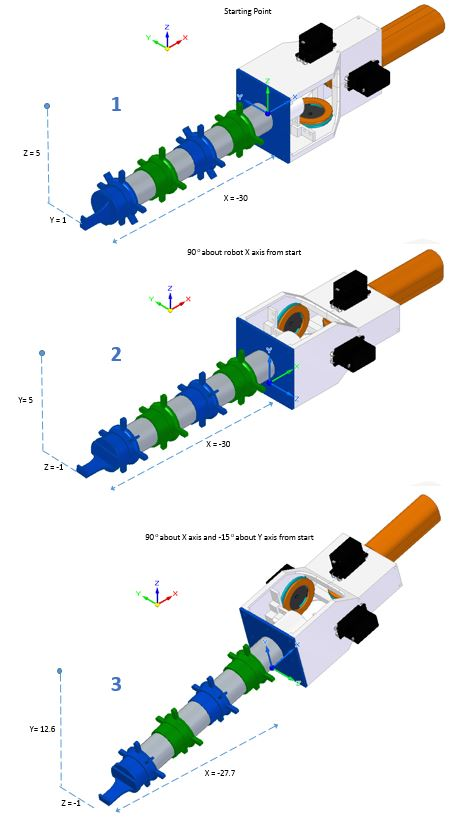
\includegraphics[width=0.83\textwidth]{images/rotationExampleAll.jpg}
\captionof{figure}{Example showing how the position and orientation of a point changes with base rotation}
\label{figure:rotationExample}
\end{center}

\begin{enumerate}
\item{The robot is in its original starting orientation, and can be said to have zero rotation about any of the axes. There is no relative difference between the axes of the robot and the global axes (shown in the top left of each image). The target point has an actual relative distance to the robot base of -30, 1 and 5 units respectively for the X, Y and Z dimensions. As there is no relative axes difference, the relative distance in relation to the robot base axes is identical in all three dimensions. As such, in this situation, the actual relative distance vector could be inserted into the regression function as is.}
\item{At the second stage, the robot has been rotated 90\degree about the global x axis. The local axis of the robot base is therefore at a relative orientation difference of the same amount. The physical relative distance of the target point to the base is unchanged, but the target point relative to the local axes of the base is different, with the local Y and Z distances being swapped around, and the latter being negated.}
\item{The final image shows the outcome if the relative rotation of the base was a 90\degree rotation about the global X axis (as in the previous image) followed by a -15\degree rotation about the global Y axis. The physical relative distance of the target point to the base is again unchanged in the global axis as the base itself has not translated in any direction. Again, the relative dimensional distances in terms of the local axes of the base are altered further, with relative values now of -27.7, 12.6 and -1 respectively for X, Y and Z. This is the vector that must be inserted into the regression function, to attain motor angles that result in a 3D point which, relative to the local axes of the base, is equal to the physical target point relative to the global and starting axes. This conversion of the target point to the local axes of the base is performed via the aforementioned steps with the negation of base angles and the rotation matrix of \ref{equation:rotationMatrix}}.
\end{enumerate}


\subsubsection{Gesturing Algorithm for Distant Targets}
In order to be cooperative and interactive in practice, a handheld robot must be able to indicate positional preferences to the user. This may entail where it must be located in order to carry out a given robotic operation, or even just the next point the user must deal with for task progression. This process is referred to as gesturing from the robot to the user towards 3D locations. In this scenario, the selected method for gesturing is comparable to typical `pointing' operations, similar to finger pointing, which is beneficial in terms of simplicity of use. Pointing is intuitive to the user as humans do this naturally to direct the attention of others to areas of interest, and is considered inherently linked to speech and communication \cite{butterworth2003}. Therefore confusion should be avoided in the user knowing where the robot desires to be relocated.

In order to gesture effectively to the user, the 3D target points must be categorised as achievable or not from the outset before deciding the next step. Initially, a point can be said to be immediately unachievable if the relative distance between itself and the base of the robot is greater than (or a certain amount less than) the typical tip-to-base distance in a straight-arm configuration. This tip-to-base distance can be used as the radius of a sphere which governs whether the points can be immediately disregarded as attainable, and requires gesturing, or whether further checking is required to assess whether it is appropriate to attempt to match this point directly. This concept is illustrated in Figure \ref{figure:tipSphere}.

\begin{center}
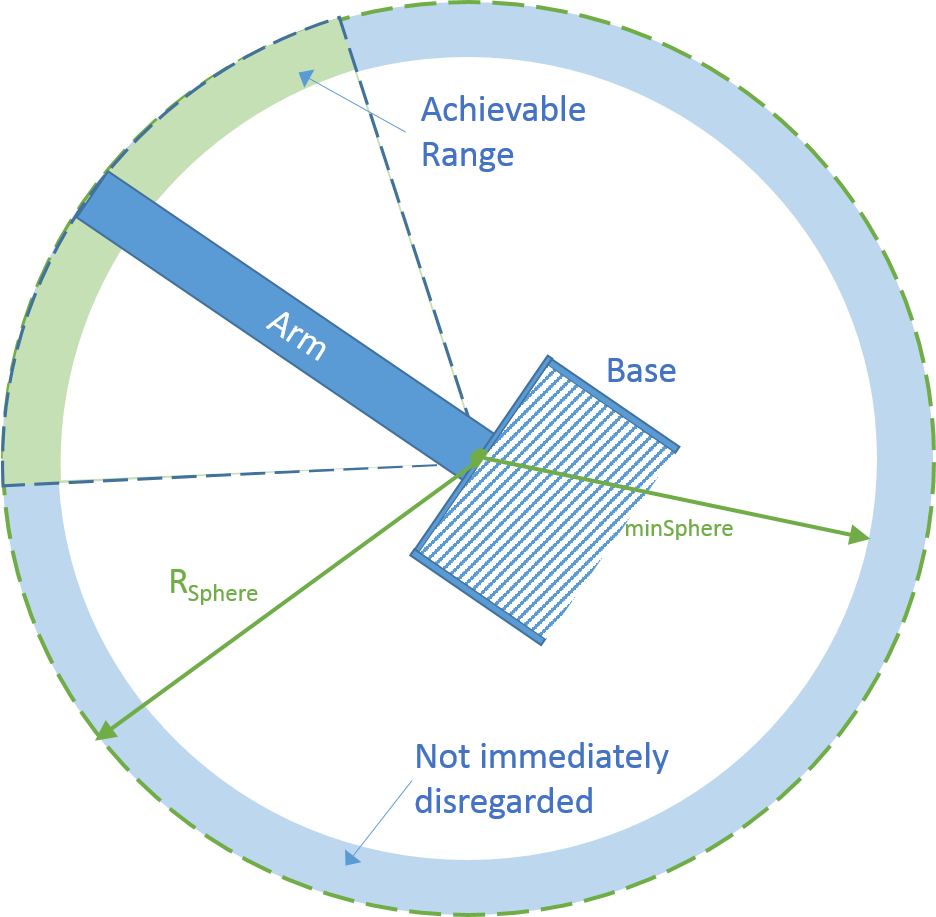
\includegraphics[width=0.7\textwidth]{images/tipSphere2.png}
\captionof{figure}{Concept of tip-to-base sphere marking immediately disregarded zone, and initial achievable range zone that requires further checking}
\label{figure:tipSphere}
\end{center}

If the point lies at an absolute distance that falls within the range between the radius of the sphere and another minimum radius, $R_{minSphere}$, the point is not disregarded as being unachievable straight away. This minimum radius is determined by the smallest absolute tip-to-base difference from the stored calibration data (3D Pythagoras). However, if it lies outside this range, a new target point is required that is equivalent to shifting the original along the vector between itself and the base until it falls in this range. 

The current target then lies within this intermediate range, and there is a further check to determine whether the coordinates of the target point relative to the base fall outside any of the recorded minimum and maximum values for the X, Y and Z dimensions. If not, then the target may be directly achievable, and the positional vector is inserted straight into the regression function to check if motor angles can be yielded, giving a solution. However in the event of this still not generating a valid solution, or if the point does fall outside any of the min/max ranges, a compromise is required. This entails selecting a new target point from the stored calibration data that is geometrically closest to the target point in question. Thus, if not able to match the point, a new point should be determined to exhibit a suitable gesture motion. The typical process for responding to a far-off point is illustrated in Algorithm \ref{algorithm:1} and a typical example is provided in Figure \ref{figure:gestureSolution}.

\begin{algorithm}
\begin{algorithmic}
\WHILE{running experiment}
\STATE{get new frame data and separate into rigid bodies}
\STATE{calculate target relative to base}
\STATE{convert target position to local axes of the base orientation}
\IF{$relativeDistance > maxSphereRadius$ \OR $relativeDistance < minSphereRadius$}
\STATE{shift along direct vector until on sphere}
\ENDIF
\IF{target falls within recorded max and min values for recorded x, y, and z positions}
\STATE{attempt direct solution from kernel regression function}
\ENDIF
\IF{3D point outside recorded max or min values \OR direct solution failed (NaN values)}
\STATE{find closest geometrical point from calibration data}
\STATE{use corresponding motor angles at this point}
\ENDIF
\STATE{set the motor angles to the solution via Arduino}
\ENDWHILE
\end{algorithmic}
\caption{General algorithm for getting from 3D target position to solution in motor angles}
\label{algorithm:1}
\end{algorithm}

\begin{center}
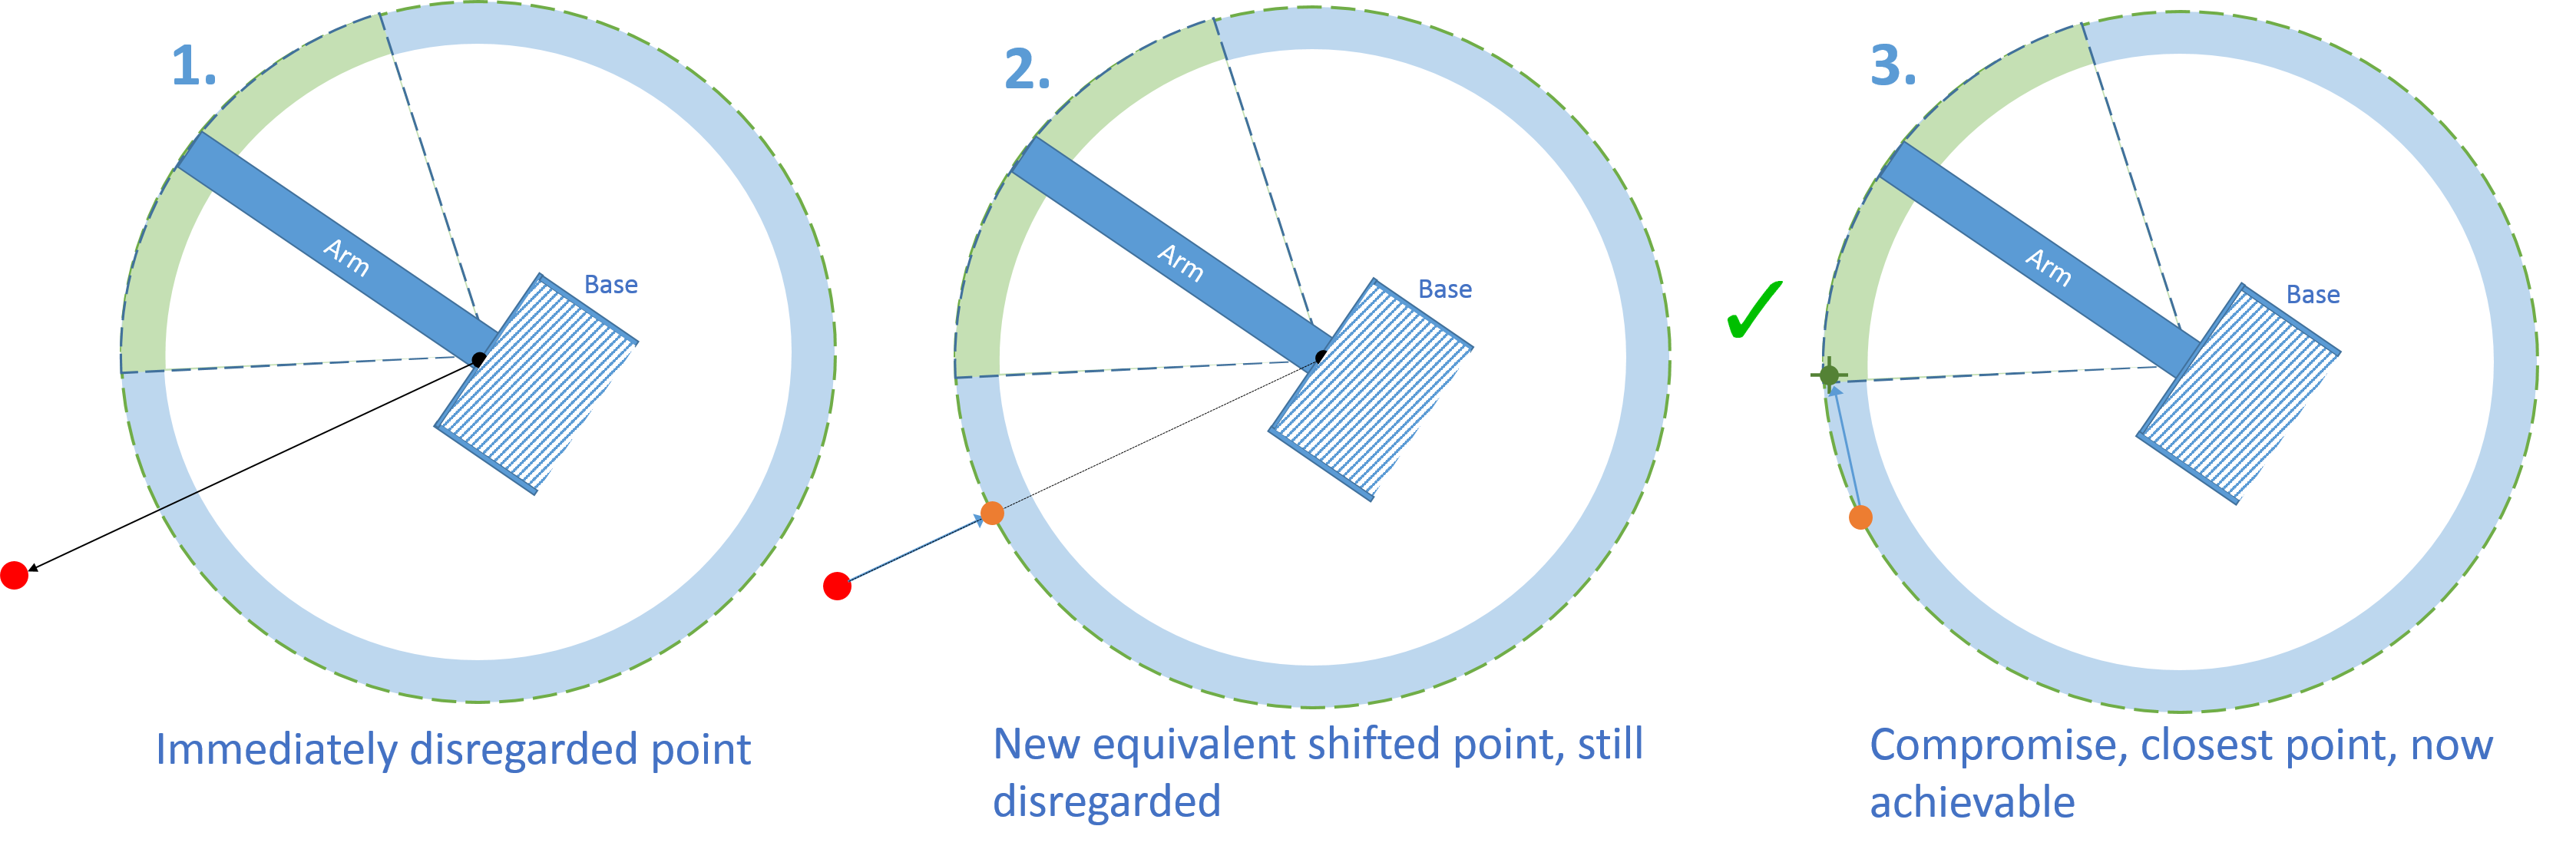
\includegraphics[width=\textwidth]{images/gestureSolution2.png}
\captionof{figure}{Typical steps in obtaining a compromised gesture solution from an initially unachievable point}
\label{figure:gestureSolution}
\end{center}


\begin{enumerate}
\item{The given target point is immediately disregarded as it lies at an absolute distance above the radius of the sphere.}
\item{A new target point is formed that is the equivalent of shifting the original point along the line from itself to the base. This is done by determining the required factor to shift the target to lie on the sphere. This factor is $Shift Factor = R_{Sphere} / absolute distance$, and each coordinate of the target point is multiplied by this to give a new vector on the sphere.}
\item{The point is still unachievable as it lies beyond the max/min range of some of the dimensions from the calibration data. The compromise is therefore to find the point in the calibration data that has the closest absolute proximity to this point and use that either as an input to the function of using the stored motor angles for this point (quicker). }
\end{enumerate}



With these steps of applying a rotation transformation and determining the best point to aim for relative to the base, there now exists a general algorithm from going from any given target point, expressed as relative to the base, and generating a solution in the form of angles to be applied to the servomotors, moving the arm to the required position, as outlined in  Regardless of the task or application at hand, this algorithm will be central, receiving inputs based on the situation and yielding solutions to be applied. This fundamental step sequence is illustrated in Figure \ref{figure:getSolution}.


\begin{center}
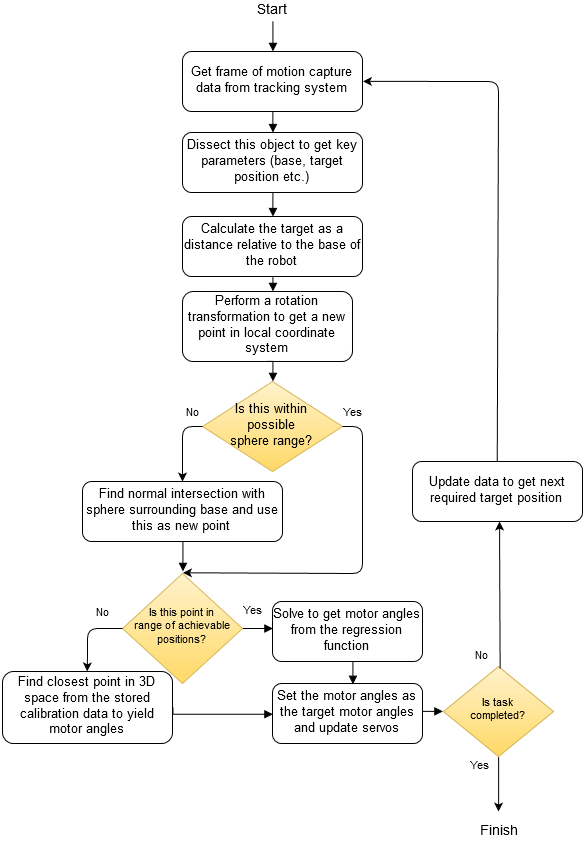
\includegraphics[width=0.75\textwidth]{images/algorithmFlowDiagram.png}
\captionof{figure}{General algorithm procedure for taking a 3D target point relative to the base and producing the most suitable solution in the form of angles to be applied to the servomotors}
\label{figure:getSolution}
\end{center}




\subsubsection{Running with a Live Target in Real Time}
In order to have handheld robotic applications, the device must be able to run with a live target in real time, always trying to move or gesture to the required position. Without this feature, the cooperation between the user and handheld robot would be seriously hindered, with the device appearing unresponsive, undermining the usefulness of the robot altogether. As such, it was imperative to set up the control of the device so that it could receive a live input, and respond accordingly to changes in its own position and orientation. This entails taking a fixed vector as a constant input, converting it to a position that is relative to both the position and orientation of the base, obtaining the solution angles vector and moving towards this target motor configuration. A simplified representation of this process is illustrated in Figure \ref{figure:separateThreads}.


\begin{center}
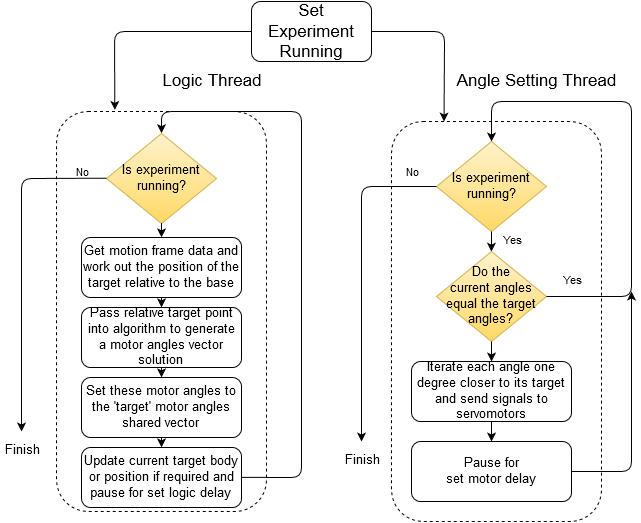
\includegraphics[width=0.85\textwidth]{images/separateThreads2.png}
\captionof{figure}{Simplified processes taking place in the two different threads, showing the servos are updated after a set interval regardless of the logic}
\label{figure:separateThreads}
\end{center}

The flow diagram shows how the control system splits this process into two threads. One thread is responsible for the logic of converting the target position and obtaining a servo configuration solution, as covered in the algorithm in the previous section. The other is solely responsible for taking the current solution for the servo configuration and iterating the servos towards this configuration (if they need to be changed). Hence these two threads share the servo configuration vector in a thread-safe manner, with the former updating it as necessary when a new solution is found, and the latter accessing it to determine how to iterate the servos towards the target. 

There is a 6 millisecond delay after iterating each servo by one degree towards its target to give a smoother motion of the arm, anything less than this was found to cause a `jerked' motion that had the potential to pull a cable loose from its pulley groove. Moreover, by iterating towards the servo configuration one degree per loop with a small delay, the effects of overshoot will be greatly reduced. By rapidly advancing towards the target, the momentum of the heavier end effector (containing the magnet) means it is more likely to carry on past its target point. Also, there is a delay at the end of the logic operation to reduce computational demand and to try and minimise rapid perturbations in the target configuration from small fluctuations in the base position and orientation etcetera. This value can be varied accordingly to alter the responsiveness of the robot at the expense of these two traits. 

This method of splitting the two tasks into separate threads, with one of them iterating the values as opposed to setting them directly is highly advantageous. As soon as the relative target is changed in real-time, requiring a different servo solution, the servos are instantaneously iterated towards this new solution. Thus, the arm does not continue moving towards an old target position, even when there is a more recent target; which may also be construed as minimising a form of overshoot where the tip moves past the current target position due to referring to a past target. This contributes towards the device appearing more responsive to an ever-changing requirement, which is essential for the practicality of a cooperative handheld robot. 

PUT CODE FOR DIFFERENT THREAD STUFF IN APPENDIX? XXX


\pagebreak
\subsection{Program Design}
The developed program for using the robot was built around the fundamentals of the Motive software and the NatNet library. An example was provided that simply sets up a connection between the tracking program and displays the tracked data in a spreadsheet. This example took the form of Windows Form Application, due to the usefulness of a Graphical User Interface (GUI) with buttons and options to start/stop tracking etcetera. Hence the developed application was of the same type, adapting the example tracking code and removing and adding features as necessary for the specific purpose of tracking and controlling the robot. This entailed creating new classes that deal with interfacing with the robot as well as the logic involved with the calibration, target selection and solving processes. 

Small tests were also added to the program so that the motion of the robot or acquiring of a solution from the regression for instance could be tested without having to fully connect to the optical tracking etcetera. This would use dummy variables where necessary just to quickly perform tests. The general process of adding a new feature to the program would entail adding a button to the GUI and attaching methods to the callback associated with it. It is often necessary to have this functionality run in a separate thread so as not to hinder the updating of data or the user interface itself (rendering it unresponsive while the operation is carried out). Hence it was essential to ensure thread safety, using a shared syncLock object when accessing shared objects, as well as delegating any user interface changes to the thread responsible for updating it. This simple user interface is illustrated in Figure \ref{figure:userInterface}.

\begin{center}
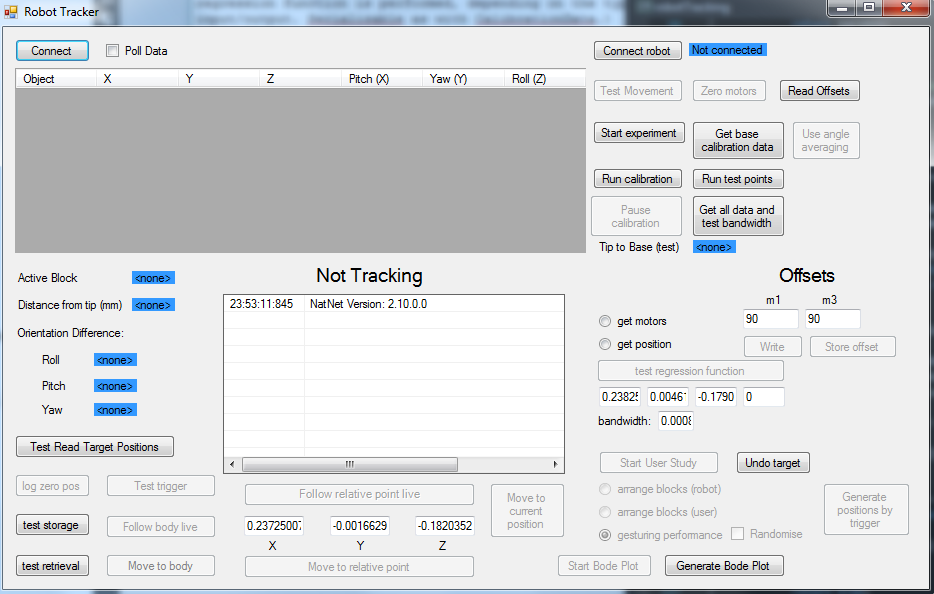
\includegraphics[width=\textwidth]{images/userInterface.png}
\captionof{figure}{User interface of the program for controlling the current status and operations of the robot, as well as for connecting to the tracking system and reading key tracking data.}
\label{figure:userInterface}
\end{center}

USE UPDATED SCREENSHOT WHEN ACTUALLY CONNECTED

The upper left and right corners provide buttons for connecting to the Motive optical tracking software and the Arduino for robot control respectively. As the typical procedures regarding controlling the robot depend on analysing tracking data and sending instructions accordingly, both connections must be established before any practical operations can be performed. Hence full connection is required to start an `experiment', which entails creating an Experiment object based on the information provided from both connections. However, as alluded to earlier, a `dummy experiment' will be created without full connection in order to provide some basic functionality so that simple motion and logic tests can be carried out without having to set up and connect to the external infrastructure associated with motion tracking. 

Other buttons are provided for both testing and essential processes. The calibration procedure is initiated, stopped and paused (in case of battery failure)for both the main calibration data as well as the test sampling, using the corresponding buttons. There's also a button for reading stored calibration data into memory, without which the regression function would be impossible. The process mentioned in SECTION XXXXXX for discovering the most appropriate bandwidth value can also be carried out here. There is a live spreadsheet section in order to display the current tracking data being recorded, such as the position and orientation of the various rigid bodies and associated markers. Similarly, labels have been added to display values that have been calculated from this tracking data, such as the absolute distance from tip to base and relative orientation. Moreover, buttons are present for performing the following test scenarios, which were especially useful during development:
\begin{itemize}
\item{Performing a basic set of movement instructions for testing the servomotors, as well as zeroing them again}
\item{Performing the regression function for an input of either the desired position or the actual motor angles for user entered values}
\item{Testing the storage and retrieval of calibration data}
\item{Moving to a relative target position, as entered by the user}
\item{Attempting to stay at a relative target position, as entered by the user, regardless of how the base is oriented/positioned}
\item{Moving to a tracked target object which is also in view of the tracking system}
\end{itemize}

The core classes of the program are illustrated in Figure \ref{figure:classDiagram}. Note that only the essential fields and methods that dictate how the program operates are shown, with the boilerplate NatNet methods, the smaller sub-methods and the less critical methods for testing and set up all excluded for simplicity.
\begin{enumerate}
\item{RobotTracker - The starting class that was built upon from the original NatNet code for interfacing with a tracking system via a simple Windows Form Application. This class is responsible for initiating the connection with the tracking system, as well as dealing with the corresponding data it receives. On top of this, it contains objects for the other main classes and methods that instantiate and utilise them. This is mostly achieved through callback methods associated with the user interface buttons, giving control to the user.}
\item{Experiment - The class that extracts the key information from the tracking data into specific variables, and performs the logic required for ascertaining the values that need to be passed into the regression function, and performing the regression itself. This entails all of the steps outlined in Section XXXX regarding converting the target orientation and finding a sphere intersection etcetera. The calibration procedure, and the loading of the calibration data, is also performed in this class, along with other test processes.}
\item{DataPoint - An object to store the motor angle vector and its corresponding relative tip-to-base position and orientation values as recorded by the tracking system. Many of these objects will make up the calibration data, and the values contained within them will be used when the regression function is performed, depending on the type of input/output. Serializable as with CalibrationData.}
\item{CalibrationData - A collection of DataPoint objects, that can be accessed as if it were an array with an index, adding and removing points as necessary. Of course, this will be serializable as it will need to be written to and read from disk.}
\item{RobotControl - This class is responsible for physically controlling the robot via its connection to the Arduino which in turn controls the servomotors. A connection is established with the Arduino and values are sent via serial connection, which are subsequently interpreted by the Arduino script and servo signals are applied accordingly. As mentioned in Section XXXXX, the values of the current motor angles are compared with their targets, and iterated one degree closer if required before being written to the servomotors together.}
\end{enumerate}

ADD ANY MORE FOR THE NEW CLASSES FOR BODE PLOT AND USER STUDY????XXXXX

\begin{landscape}

\begin{center}
\includegraphics[width=1.4\textwidth]{images/classDiagram.png}
\captionof{figure}{Core classes and their associated fields and methods that are central to how the program runs.}
\label{figure:classDiagram}
\end{center}


\end{landscape}



\section{Evaluation}

In order to evaluate the new handheld robotic device, it was important to identify the key characteristics that need to be identified so that the aims of the project can be achieved. This project is primarily focused on the design of a new device, and importantly, how it can utilise pre-acquired task knowledge to effectively cooperate with the user. Specifically, it is the alleviation of cognitive effort that is of concern, as this demonstrates the notion that operators unskilled or untrained in a certain task could achieve the objectives regardless through assistance from the robot. Therefore it is essential to highlight this ability, and as such, a user study was to be carried out to compare the completion of a mentally demanding task without mental assistance from the robot, to a physically similar task where the cognitive burden is dealt with by the device, gesturing to the user the required actions.

The physical performance of the robot is of much less importance in this project, based on the design and construction taking place over a much shorter time-scale than is typical for robotics. However, it is still necessary to evaluate certain traits that would directly affect how effectively the robot can gesture (or cooperate) with the user. These traits could be dependent on the mechanical design of the robot, or the underlying algorithm and data that governs how the robot responds. Therefore, it was important to quantify the control performance of the robot in terms of step and frequency response. To complement the user study evaluation, it is also beneficial to test how effectively and accurately the robot can gesture to specific target points. Therefore an experiment was set up to ascertain how reliably desired physical locations can be conveyed to the user. 
\subsection{Experimental Procedure}

\subsubsection{Response Performance}
In order to measure the response of the robot to various target inputs, it was necessary to constrain the robot and assign a live target that could be varied accordingly. As such, the robot was clamped in place using a vice, similar to the calibration procedure in SECTION XXXXX. The OptiTrack Duo was then set up to have a clear view of the both the base and tip of the robot. Then, in the motive software, a new rigid body was defined using a small `wand' made up of three-markers, as illustrated in FIGURE XXXXX. The pivot point of this rigid body was then set as one of the single markers, giving an actual visual indicator in the real world of the 3D point that is being tracked.

PICTURE OF WAND SHOWING WHICH POINT WAS MADE PIVOT POINT? XXXXXX

The absolute position of this wand, as ascertained by the optical tracking and assigned to the field of a rigid body object in the program, could then be extracted with each frame and used as the input to the general algorithm, converting it to a relative target position in the local axes of the robot and obtaining a motor angle solution. Of course, the multi-threaded technique of ascertaining the solution while simultaneously iterating the motor angles towards whatever happens to be the current solution, as covered in SECTION XXXX, is also used so that the wand could be used as a live target for the arm to follow.

Once in place, the wand was held at a point deliberately outside the range of possible solutions from the robot, meaning that it had to use the closest calibration point to gesture in that direction. This point was outside the range in both the X, Y and Z dimensions so that the point that the robot moves to for gesturing is repeatable; even if there are small differences in the position of the wand, as long as it is consistently outside the range of recorded values in the same directions each time then the robot will gesture at the same point. In this case, the starting position of the wand would be up and to the right, if looking at the robot head on down the axis of the arm. The wand could then be moved vertically down to another point outside the range of solutions (to the right and down) causing the program to find another set of solutions as it moves down. As long as the wand is always kept outside the possible solutions in the X direction, it should follow a vertical path downwards to the new max range gesturing position, while remaining at its maximum X position the whole time. Again, this makes the motion more repeatable, in that as long as the wand follows roughly the same path each time, the arm should follow the same exact path. This experimental set up as well as the motions of the target and the arm is illustrated in Figure XXXX.

INSERT TWO SIDE BY SIDE IMAGES OF THE ROBOT IN THE CLAMP WITH THE WAND IN THE UP RIGHT, THEN ANOTHER WITH THE ARM HELD IN THE LOWER RIGHT, SHOWING THE ARM IN ITS NEW POSITIONS WITH ARROWS TO SHOW WHICH DIRECTION THE ARM JUST MOVED XXXXXX

Once this was set up and the arm could follow the motion of the target wand, gesturing when it was out of range. The subsequent steps were to record the response of the arm. This procedure necessitates the logging of the positions of the target and tip at a range of time steps. Therefore, when starting a response plot by clicking the appropriate button on the GUI, a timer would start and the robot would commence following of the target wand. At each interval of around 50ms, the positions of the wand and tip were logged. Finally, once the response plot was stopped, the recorded data was written to a csv file for graphing. 

This process was carried out for two types of response, where the Y positions of the target and tip could be plotted as they are the key variables for the input motion. Firstly, a step response was performed, where the target was held still in the start position then moved rapidly down to the next point, roughly within the window of the logic delay before the program attempts to solve for the next target position. Finally, the positions were recorded while the target wand was moved up and down at a roughly constant frequency. This was then repeated at higher frequencies, until anything higher would be difficult to perform by hand while maintaining a constant rate. In total, eight different frequencies were used to perform a basic assessment of the frequency response.


\subsubsection{Effectiveness and Accuracy of Gesturing}

In order to assess how effectively the robot could gesture to a target, a small experiment was to be carried out. This had to provide a means of ascertaining whether the device could accurately convey its desired location to the user, when other potential targets were nearby. As such, the user should be able to differentiate between the correct targets and its neighbours, which would be imperative in alleviating mental workload. The experiment set up for this procedure was based around moving to physical target bodies; these were selected as lightweight foam blocks. The blocks were 7cm in width and height, with the depth ranging from 3.5 to 7cm. The depth is of less importance as they were to be arranged in such a manner that the robot gestures to the centre of the front face, giving a target surface area of 49$cm^{2}$, which is thought to be a typical target area for manoeuvring physical objects in applications that don't require identifying targets in a high precision environment, such as identifying correct blocks in a construction scenario.

The blocks were to be arranged in a four by four stack, giving a total of 16 blocks in a wall that was 28cm by 28cm. Then, using the technique mentioned in SECTION XXXX(the program design section), the 3D target points, corresponding to the tip of the robot being at the centre of the front face, were to be obtained for each block. In order to minimise any errors, uncertainties, or potential accuracy limitations of the OptiTrack Duo, the best position to place the camera would correspond closely to the same relative location to the device that it was at during the calibration procedure. This took place with the robot angled at about 45\degree to the front of the Duo, so that it maintained a clear view of the markers on the tip and the base at all calibration points. Therefore, so that the response of the robot does not hugely depend on how accurately the Duo can give the relative orientation of the device to when it was calibrated, it was to be placed in a similar relative position in practice. The physical setup for this experiment is thus illustrated in Figure XXXX.


INSERT PICTURE OF THE FULL WALL OF BLOCKS, SHOWING THE ROBOT FACING THE WALL, MAYBE STRAIGHT MAYBE GESTURING TO A BLOCK, AND HAVING VIEW OF THE CAMERA, LABELLING IT AS OPTIMAL POSITION XXXXXXXX




The position determination procedure entails tracking the tip, positioning it in the desired location, and pressing the trigger to log the current coordinates to file. However, this can have issues when considering the optimal position of the optical tracking device. The problem then arises from visibility of the tip during this target position logging procedure. With the duo positioned optimally for accuracy, it cannot maintain line-of-sight with the tip once it passes behind the wall of blocks. As such, the 3D locations had to be logged without having every block in place. A compromise then, was to assemble only the vertical stack on the furthest side. When the tip was lined up with these blocks, there are no other blocks obscuring the view from the camera, so they could be logged accordingly. Then, by pre-marking the centres of each column on the surface that the blocks sit, this end column could be shifted over by the width of one block, representing the next closest column, and the positions logged. The process is repeated until all 16 positions have been logged, before placing the actual blocks in their correct positions. This procedure is illustrated in Figure XXXXX.

INSET PICTURE OF END COLUMN BEING LOGGED , WITH DASHED LINES TO SHOW POSITIONS OF WHERE NEXT COLUMN WOULD BE. MAYBE TWO SIDE BY SIDE OF COLUMN BEING MOVED OVER TO NEW POSITION, WITH TICKS WHERE THE COLUMN USED TO BE SHOW THAT THEY HAVE BEEN LOGGED XXXXX

Of course, the issue of tracking the tip would then reoccur once the wall is fully in place. To move the tip towards the target position, the algorithm only needs to know this position relative to the base, which it will then utilise the calibration data to obtain a motor angle solution that should result in the tip moving to the same (or the closest to) relative point. Therefore, in order to actually respond to target inputs, the program does not need to know the actual position of the tip at all. Therefore, when carrying out this experiment, the Motive software was re-configured to only track the base of the robot, which, when positioned so the tip can move towards targets, will remain far enough from the wall so to be visible at all times by the Duo. 

The logged positions were arranged in such a manner that the bottom right of the wall (as viewed by the user) would corresponding to the first position, with the next position one to the left and so on. Upon reaching the end of a row, the subsequent position in the order would be the block at the right hand edge of the next row up. This order was referred to by zero index, with the bottom right block assigned to 0 and the top left assigned to 15, so that the positions can be loaded from file into an array of 3D vectors, and the notation for the physical order will correspond to the indices of the coordinates array. 

Then, when performing the experiment, the stored block positions are loaded into the array, and a new array of five integers is formed by selecting random values from 0 to 15, representing a random order of positions of blocks. A new array of five target positions is then created, by accessing the stored positions at the indices according to the array of integers (position notations). An example of this random sequencing is illustrated in Figure \ref{figure:gridSequence}. The operator has no indication as to what this new sequence of five targets is, except for the arm gesturing to the next target. The user could then move the arm so that the tip reaches its desired point, and state which block index position they think is the current target. Clicking the trigger then serves to move on to the next target position in the random order, and the process is repeated until all five targets have been cycled through. Once the experiment is stopped via the GUI, only then is the random order of position indices revealed, so that the order suspected by the user can be compared with the actual order, revealing how reliably the positions were conveyed by the robot gesturing.

\begin{center}
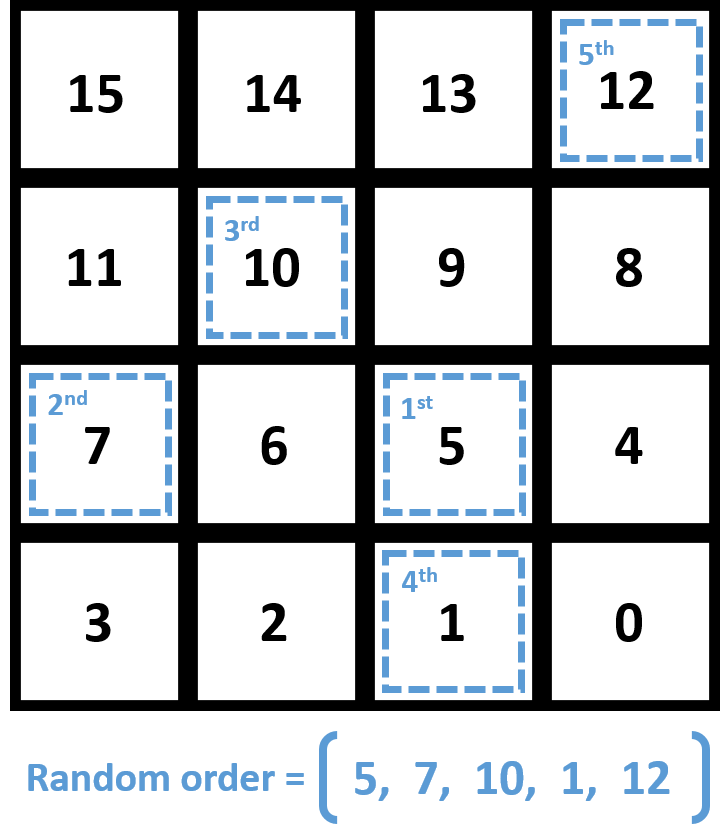
\includegraphics[width=0.5\textwidth]{images/gridSequence.png}
\captionof{figure}{Positional order of the wall of the blocks as observed from the front, denoted in black, and an example of a randomly generated order of positions for the experiment, denoted in blue.}
\label{figure:gridSequence}
\end{center}



\subsubsection{Alleviation of Cognitive Workload in Users}
MENTION THE USER STUDY CLASS OF THE PROGRAM THAT TAKES TRIGGER CLICKS AND LOGS THE ABSOLUTE POSITION OF THE TIP INTO A CSV FILE XXXXXXX

Given the aims of the project, it was imperative to investigate whether the device could actually perform its intended function and further prove the potential for cooperation between humans and handheld robotics. Specifically, its ability to draw on task knowledge to interact with the user to reduce perceived mental workload must be evaluated. The most appropriate way to carry out this evaluation entails a live user study, in which participants use the robot in practice, and specify the extent to which it mentally assisted them. As such, an experiment was designed in which the users would perform two tasks using the robot to place coloured blocks in a specific order into a box. This was accomplished by attaching metal strips to seven of the foam blocks from the gesturing effectiveness experiment, and setting the program so that the electromagnet was activated and the arm held straight when the trigger was held down. Coloured stickers were then attached to the front face of the blocks to give seven unique blocks: red, orange, yellow, green, blue, white and purple, which were then placed in a straight horizontal line at the front of the table. As the physical accuracy was not under investigation here, a conservative spacing between blocks was selected at 7cm.

PICTURE HERE OF THE BLOCKS ON THE TABLE AND BOX BENEATH? XXXX

One of the tasks entailed dispensing the blocks in a sequence that required conscious cognitive effort in order to follow correctly, where the arm of the robot remained straight for the duration of the task. The only response to the trigger in this case was to activate the magnet. The instruction for this sequence was to place the blocks in an order that was alphabetically ascending for the \textit{third} letter of the colour. That is, A comes before B, which was made clear to the user when informing them of the sequence instruction. Only six of the blocks were to be dispensed, with the final one to be left on the table, serving as a dummy. Once the instructions were acknowledged by the user, a timer was started and the order of the blocks they dispensed was recorded, with the timer being stopped after the sixth colour entered the box. The correct order was thus:
\begin{enumerate}
\item{OR\underline{A}NGE}
\item{RE\underline{D}}
\item{GR\underline{E}EN}
\item{WH\underline{I}TE}
\item{YE\underline{L}LOW}
\item{PU\underline{R}PLE}
\end{enumerate}

However, if an incorrect block was selected, it would only count as a single error. That is, after an incorrect block, the score would then be based on the correct ordering of the remaining blocks, whatever they may be. Before the task, it was important to ask the user if they were colour blind, or non-native speakers of English, and note it if so. They were then asked to verbally state what colours were laid out.

For the other task, a pre-defined order of six blocks was created, as before, by moving the tip to the target positions and logging it with the trigger. Again, visibility issues were encountered when all of the blocks were laid out so markers were put in place and only one block was used to log the positions, moving it between the markers. The base was again the only rigid body tracked during the experiment, for the reasons mentioned in the gesturing effectiveness experiment. The users would then be unaware of this order, and upon commencing the task the timer would be started and the robot would gesture to the next target. When the trigger was held, the magnet would activate and the arm would straighten up for easier manoeuvring of the blocks. Once the trigger was released, the arm would then begin to gesture to the next target, until after the sixth target when the experiment would stop and the arm would remain straight. Of course, if the trigger was released accidentally, the arm would move on against the user's wish. Therefore a button was added to the GUI to effectively `undo' the trigger press and move back to the previous target. 

Before the assisted task commenced, a brief demonstration was given to the user, using a different and shorter pre-defined sequence, and they briefly practised using the robot while it gestured to a target. If, in the real task, an error was made and an incorrect block was taken, difficulties may arise, where the robot could later gesture to an empty space. In this event, a spare block would be placed in the empty space for picking up. These spare blocks were uncoloured as, due to the nature of this task, the colours are unimportant as it is the order of positions that is logged. So a single erroneous selection would only count as 1 mistake, providing the following order of selections were correct.

Upon completion of both tasks, a modified TLX form was then given to the participants to fill out. As covered in Section XXX (TLX), this covered the key perceptions of task load; mental demand, temporal demand, perception of performance, total effort, frustration and physical demand. The latter is of little importance in such an investigation, with the two tasks expected to be identical in this regard, but was included for completeness nonetheless. This was filled out for \underline{both} the mentally assisted task (gesturing) and the colour sequence (unassisted) task. This modified TLX is given in APPENDIX XXXX. 


\pagebreak
\section{Results and Discussion}
\subsection{Response Performance}
\subsubsection{Frequency Response}

After analysing the positional data for the results, the actual amplitude of the motions of the target and the tip of the arm could be ascertained. It was found that for the the frequency response experiment, the amplitude of the target motion was mostly constant, as intended, at around 175mm (350mm peak to trough). As mentioned earlier, this amplitude was larger than the capped vertical range of motion of the arm, so that the arm moved from gesturing position to the other. The mid-point of the motion of both bodies was roughly at the same point in the Y direction, giving an equally distant target position on each side of the centre of the robot. The maximum amplitude of the arm in terms of the half the distance between the maximum and minimum Y positions from the calibration data (maximum cable tension) was recorded at 75mm. Hence an extra clearance distance of around 100mm would be present on each side of the arm from the target wand when stationary at the extreme values. 

The target wand was found to oscillate at a range of eight frequencies from 0.4 to 2Hz. This was calculated by measuring the average time between peaks of the target motion, giving the wavelength, and using the standard equation:
\begin{equation}
frequency(Hz) = \frac{1}{wavelength(seconds)}
\end{equation}

At each recording, a portion of the physical response graph would be identified where the frequency was mostly constant, as shown in EXAMPLE IN APPENDIX XXXXXXXX, from which the amplitudes of the tip could then be calculated and averaged (the amplitude of the target was roughly constant). The magnitude of the tip amplitude in relation to the target amplitude was then converted in to decibels using the average values at each frequency with the following standard equation, and the resulting bode plot for the amplitude response is shown in Figure \ref{figure:amplitudeResponse}.

\begin{equation}
magnitude(dB) = 20\log \left(\frac{tipAmp}{targetAmp}\right)
\end{equation}

SHOULD THIS BE IN RELATION TO THE MAX TIP AMPLITUDE INSTEAD OF THE AMPLITUDE OF THE TARGET, SO THAT WHEN THEY ARE EQUAL IS IS 0DB, GIVING A MORE LOGICAL REPRESENTATION, AS FAR AS THE ROBOT IS CONCERNED THE TARGET ONLY GOES FROM THE MIN TIP POS TO THE MAX TIP POS ANYWAY AFTER IT IS CONVERTED? OR DOES IT HAVE TO BE THE TARGET AMPLITUDE BECAUSE THAT'S THE WAVE AND FREQUENCY THAT THE TARGET ACTUALLY WENT THROUGH??? OR PUT A SEPARATE LINE ACROSS THIS GRAPH AND ANOTHER DIFFERENT COLOUR PLOT BENEATH IT TO SHOW WHAT IT WOULD BE LIKE IF USING THE MAX TIP AMPLITUDE INSTEAD OF ACTUAL TARGET AMPLITUDE XXXXXXXXXX

\begin{center}
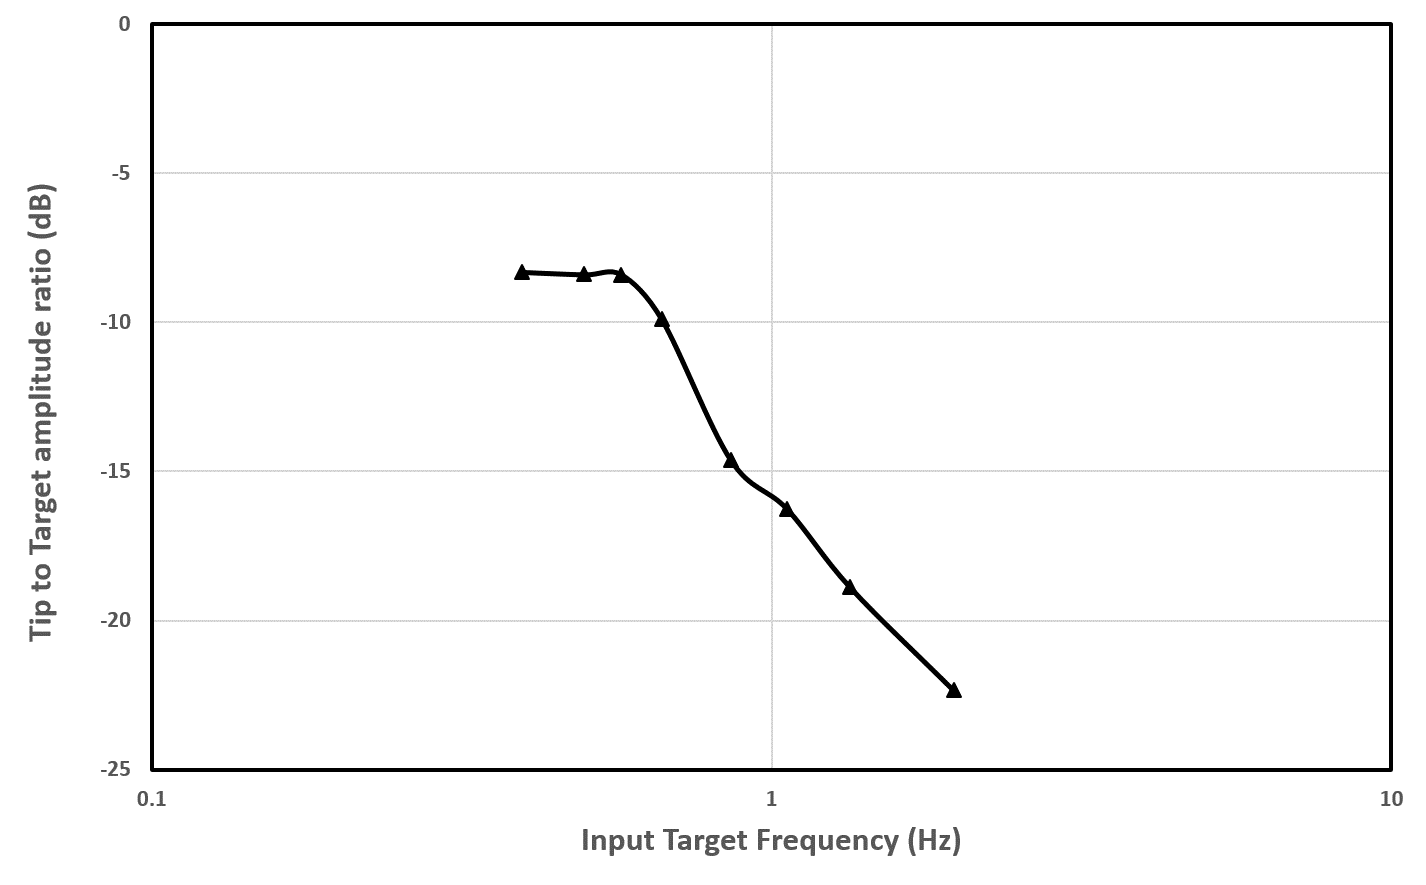
\includegraphics[width=0.8\textwidth]{images/amplitudeResponse.png}
\captionof{figure}{Ampltude response (in dB) of the tip to varying target frequency.}
\label{figure:amplitudeResponse}
\end{center}

DISCUSS THIS AMPLITUDE PLOT ONCE DECIDED WHETHER TO PLOT USING TARGET AMP OR MAX TIP AMP XXXXXXXXX


\pagebreak
The phase shift of the tip in relation to the target could also be calculated for each constant frequency portion of a recording. This was done by averaging the time between the peaks of the target and tip, to obtain a time lag in seconds, and using the following equation:

\begin{equation}\label{equation:phaseShift}
Phase \ shift \ (degrees) = -1 \times lag(seconds)\times Frequency(Hz)\times 360(degrees)
\end{equation}

This phase shift between the target and the tip of the arm was then plotted for the frequencies, as illustrated in Figure \ref{figure:phaseResponse}.

\begin{center}
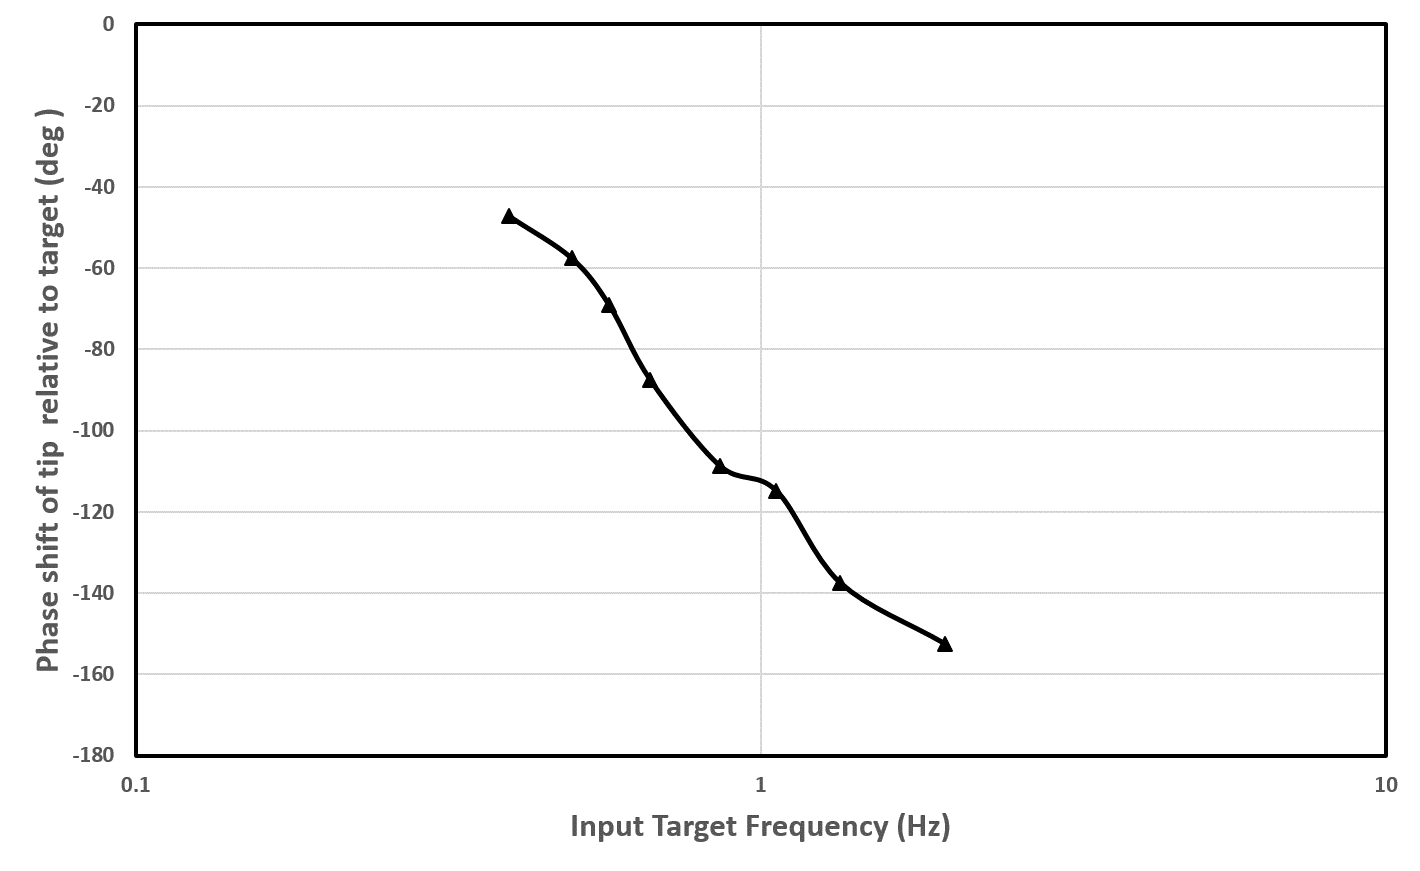
\includegraphics[width=0.85\textwidth]{images/phaseResponse2.png}
\captionof{figure}{Phase shift response (in degrees) of the target motion to tip motion for varying target frequency.}
\label{figure:phaseResponse}
\end{center}

As shown in the phase plot, there is a considerable phase lag for the tip to respond to the target when the frequency of the target variation exceeds 1Hz, with the lag approaching 160 degrees around 2Hz. The naive view here would be to categorise the device with low performance based on these figures. However, it is important to consider the actual context that the device is intended to be used in. The device was designed with the intention of utilising a task knowledge to alleviate the mental effort of its operator. It does through the act of physically gesturing to the desired location. Therefore, in such a scenario, where the user requires the robot to gesture to the next target, it is not as critical to have a rapid response when this target changes. Situations where this physical target change may occur will be typically events where the user carries the device towards the target direction and slightly overshoots the target so the device must now gesture in the opposite direction. Such physical acts are unlikely to occur at frequencies much higher than 1Hz, and will therefore not pose serious problems to usability. 

The tasks such a robot would be expected to assist with, and what it was designed to prove, would not require complex mechanical motions in a rapidly changing environment, instead benefiting more from taking away the mental workload which would otherwise be taxing. If the physical performance was imperative, the frequency response may in such case prove unsatisfactory, hindering the performance and benefits offered by the robots as a whole. For this project, it was decided to strike a balance between responsiveness and maintainability by setting the aforementioned motor delay (the delay after each individual servo is incremented by one degree before incrementing the next one) at 4 to 6ms. This was the highest delay found to still move the robot at appropriate subjectively acceptable speeds. This value was explored, being taken down to as low as 1ms where much greater speeds were observed, although reducing it beyond the selected amount was found to induce new problems. 

At such small delays ($<4ms$), the rapid motion of the servos was found to vibrate the servo horn, at the centre of the pulley, free from the servo shaft, requiring instant repair. In the worst-case scenario, the servo horn was found to shear loose from the glue connecting it to the pulley, which resulted in a lengthy downtime. These two issues came about from two flawed factors of the design; not screwing the horns to the rear servos due to accessibility issues, as well as using relatively weak glue for the pulleys on account of the rarity and potential need for re-use of the specific circular servo horns.  

With more emphasis on the physical performance, changes could be applied to the design of the robot to allow access to screw the pulleys to the rear servos, as well as replacement servo horns delivered to allow high-strength glue to be used on the pulley, addressing both of these problems. However, these relatively simple to implement changes would have added more time onto the design phase of the project, which was already strictly capped by the project time-frame. Although the robot could potentially endure the duration of this experiment at the minimal delay, the response was not investigated at such speeds as a fair representation could only be given if tested at the same speed that will be experienced when actually using the robot in real task scenarios. An example scenario that is considered commonplace in such mentally assisted tasks is illustrated in Figure \ref{figure:baseOvershoot}.

\begin{center}
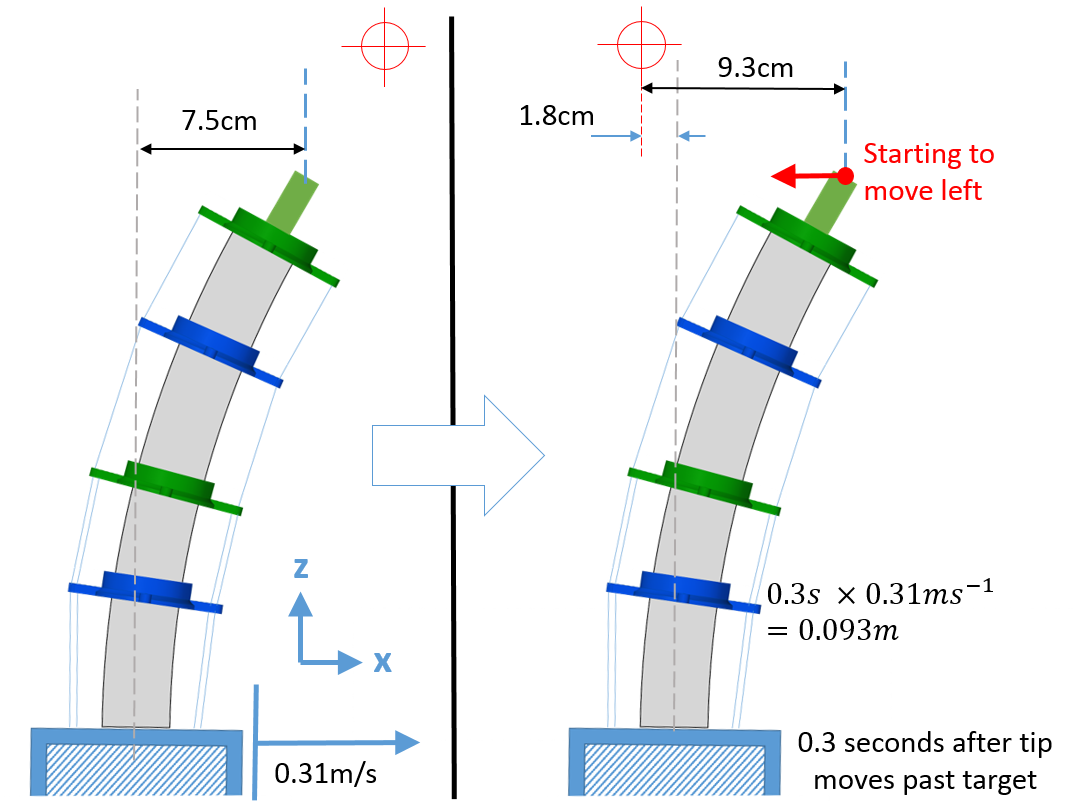
\includegraphics[width=0.95\textwidth]{images/baseOvershoot.png}
\captionof{figure}{Example of typical conditions expected the robot is expected to be subjected to when mentally assisting with tasks, simplified to X translation only, showing potential base overshoot.}
\label{figure:baseOvershoot}
\end{center}


It is assumed that in typical applications for this robot, a changing target would not move at a rate from the extreme tip positions at a rate above 1Hz. This is comparable to saying that in half a second, the target position would move across the range of tip motion, which in such a case would be at a speed of 0.31m/s. The phase lag at 1Hz, as obtained from the raw data or Equation \ref{equation:phaseShift} and the graph, would be 0.3s (or 114\degree). In an environment where mental assistance is the primary concern and gestures are responded to, this target change relative to the base could come from moving the device past the target at a fixed orientation, rotating it so the target moves relative to the orientation of the base, or a combination of both.

For simplicity the diagram assumes a fixed orientation translation of the robot towards a gestured point out of range to the right. Eventually a point will be reached where the tip and the target are equal in terms of the X dimension. This in itself can indicate to the user that robot has just passed the target position in that direction, allowing them to intuitively ascertain the general target area, which may be sufficient to locate the target if there are few possibilities in that region, or they may have to wait a little longer for more precise gesturing. Either way, they should logically stop moving. In this case, the base would continue to move after the tip passes the target for 9.3cm, which is about 1.8cm more than the tip would be from the base when gesturing (7.5cm), so the base would roughly only overshoot by a maximum of 1.8cm  from the point in line with the target, when the tip starts to move and the user halts. Considering this information as a typical case, where the robot would rarely move faster than this and would also usually be oriented towards the target direction, reducing the overshoot further, the robot appears suitably responsive. Hence this frequency response is deemed appropriate for a robot with the remit of assisting with mainly mentally challenging tasks in a physical environment. 



\subsubsection{Step Response}

Using the same setup as for the frequency response test, a step response experiment was also carried out. The target wand was moved as fast as possible from one extreme position to the other, and the arm was allowed to fully move to the new position and settle before the subsequent step input. The positions of both bodies along with the current timer value were then logged as before. The resulting step response in terms of absolute position against time in the Y direction is illustrated in Figure \ref{figure:stepResponse}.

\begin{center}
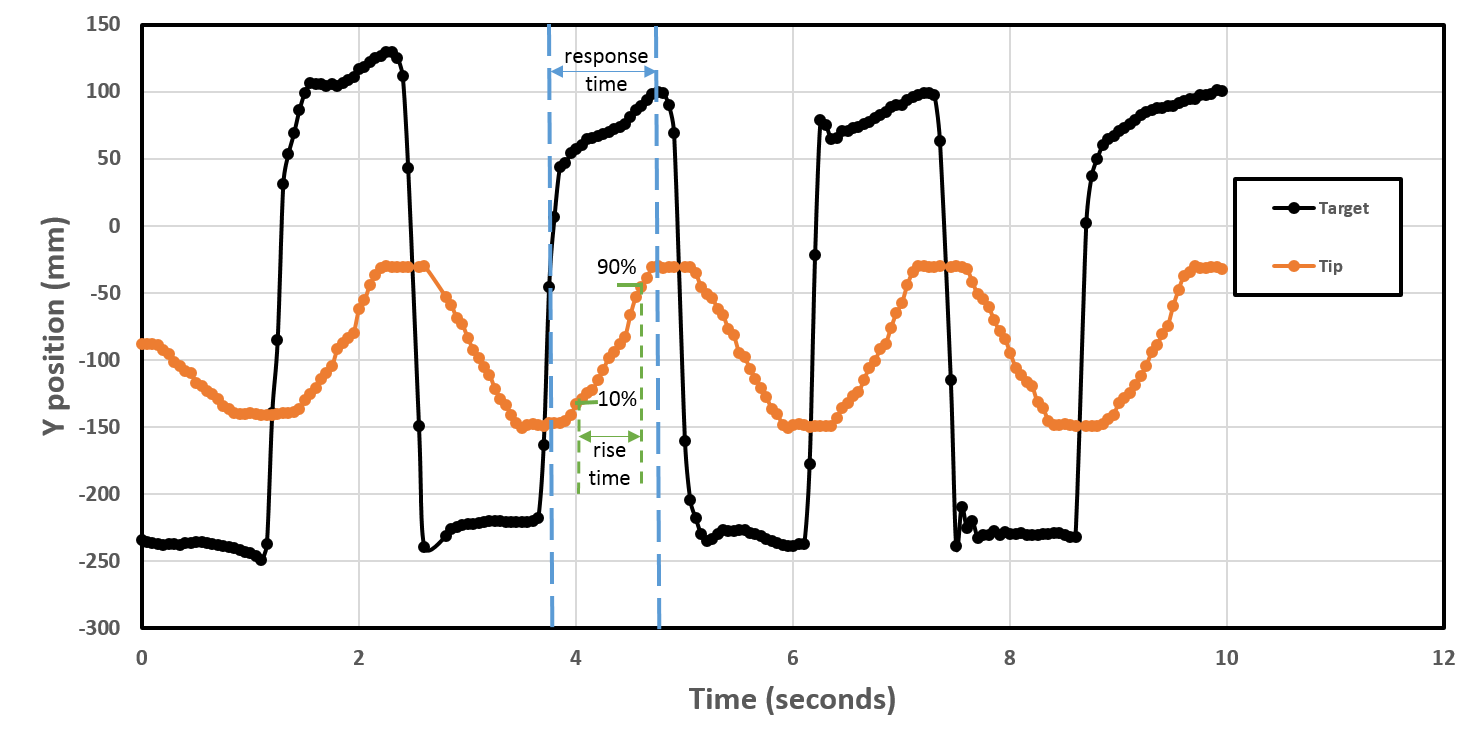
\includegraphics[width=\textwidth]{images/stepResponse.png}
\captionof{figure}{Physical response of the tip in the Y direction to a step input from the new target position.}
\label{figure:stepResponse}
\end{center}

Unlike in traditional control systems, there is no specific transfer function, expressed as an equation with the input signal, that the robot adheres to. Rather, the algorithm of setting the servo angles relies on checking the most recent solution, comparing the current angles with these values, and iterating the servos closer to the solution one degree at a time with a slight delay after each step. This process was covered in more detail in SECTION XXXXXXX. As such, with a stationary robot, the servos themselves cannot technically overshoot. Once they reach the target angles (in degrees), the program will not iterate them any further. Of course, the tip itself could overshoot past its target based on the momentum of the end effector when the servos stop moving and the flexibility of the arm. However, when the motor delay was experimented with, the range of 4 to 6ms was found to provide smooth motion without any tip overshoot upon stopping. Also, overshoot may occur as a result of the human moving the tip past the target quickly so that it has to change direction, though this is not related to the step response of the robot itself. 

Given this way in which the robot responds to target positions, eliminating servo overshoot, the most comparable level of damping that the robot is subjected to, in terms of typical control system terminology, would be `over damped'. This implies that the servos could move at a greater speed than they do, while still reaching their target without any overshoot of themselves or the tip, which is a fair assumption. As such, it is common practice to quantify the rise time of the step response as the time taken for the response to move from 10\% to 90\% of its target motion. This is labelled in the step response graph. As such, this time was found for each step input that was recorded, and averaged to give a rise time value of 0.62 seconds. The total response time, that is, the time taken from the step input (one extreme to the other) until the arm moves to its new steady state position, was found to average at 1 second exactly. 

If one considers the remit of such a device, with the user finishing a current operation, resulting in a new target position, the maximum time they will have to wait before the robot moves to the new gesturing position is only a second. Given the user could also intuitively see which direction it's `starting' to gesture in, the robot can therefore be said to appear suitably responsive. Of course, a more reliable evaluation of the cooperation between the operator and device can only be given by results the robot being used in practice by real users.

\subsection{Effectiveness and Accuracy of Gesturing}

For the gesturing effectiveness experiment, the test was repeated with one user for a total of 14 times. The stated positions, for the randomly generated list of five indices, were recorded along with the actual values printed by the program at the end of the test. Therefore, a total of 70 random target positions were issued. The resulting stated XXXXX

\begin{center}
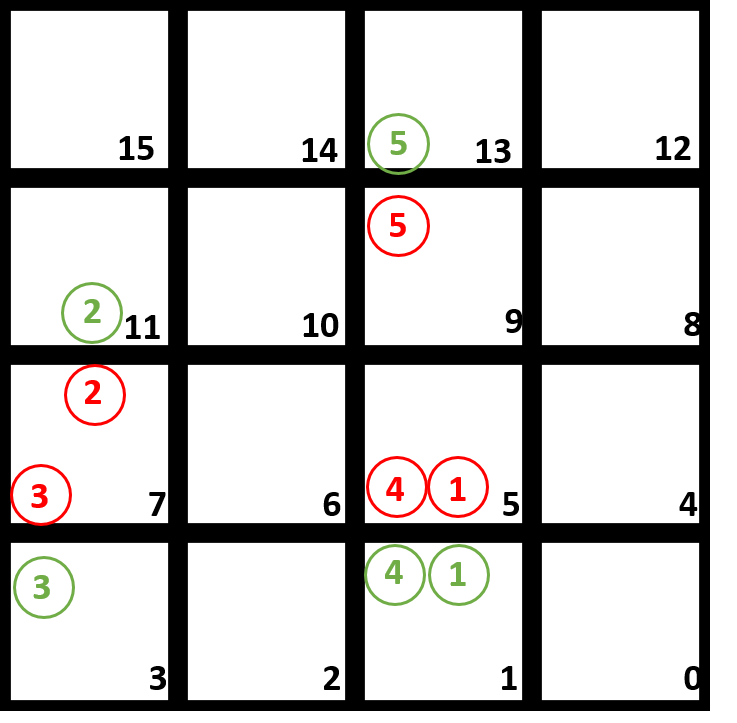
\includegraphics[width=0.55\textwidth]{images/gestureErrors.png}
\captionof{figure}{Recorded errors for the gesturing effectiveness experiment, shown by the matching numbers with green for the correct position and red for the stated position.}
\label{figure:gestureErrors}
\end{center}

\subsection{Alleviation of Cognitive Workload in Users}


\section{Conclusion}
WERE AIMS AND OBJECTIVES MET, WHAT ELSE WAS FOUND OUT????
\section{Further Work and Areas of Improvement}
\subsection{Physical Design}
\subsection{Evaluation}

\pagebreak
\bibliography{mybib}
\bibliographystyle{unsrt}

\pagebreak
\section{Appendices}
\subsection{CAD Drawings}
\subsection{Servomotors}

\begin{center}
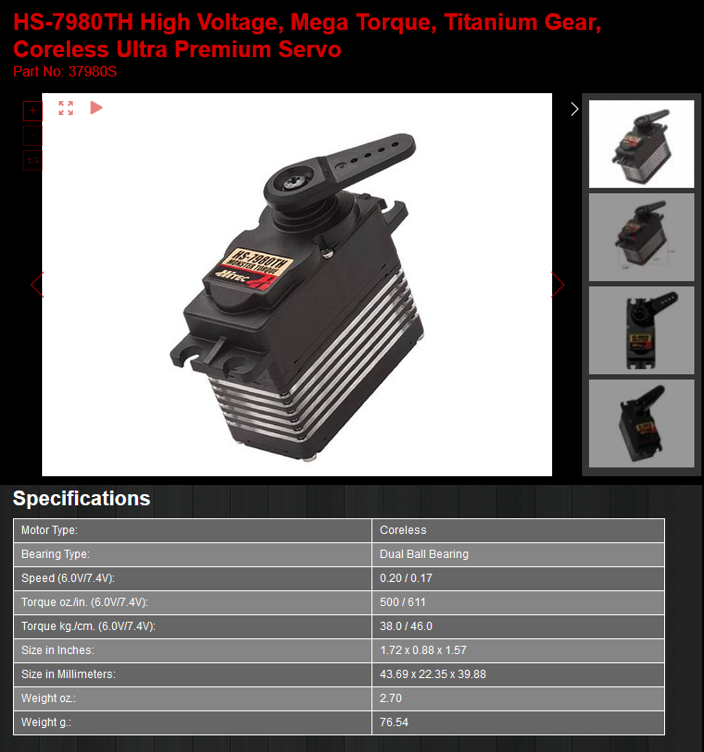
\includegraphics[width=0.8\textwidth]{images/servoSpecs.png}
\captionof{figure}{Specifications for the Hi-Tec HS-7980TH Monster Torque Servomotors used on the robot.}
\label{figure:servoSpes}
\end{center}


\subsection{Tracking Device}
\subsection{Arduino Board}
\subsection{Code Snippets}
Put code for writing the motor angles to the servos, perhaps starting the new thread that just continuously writes the angles. Perhaps code for starting an experiment and tracking the bodies, getting the information out, and using them as a target. Also perhaps the regression function code? XXXXXXX

\subsection{Gesturing Effectiveness Results}

\begin{center}
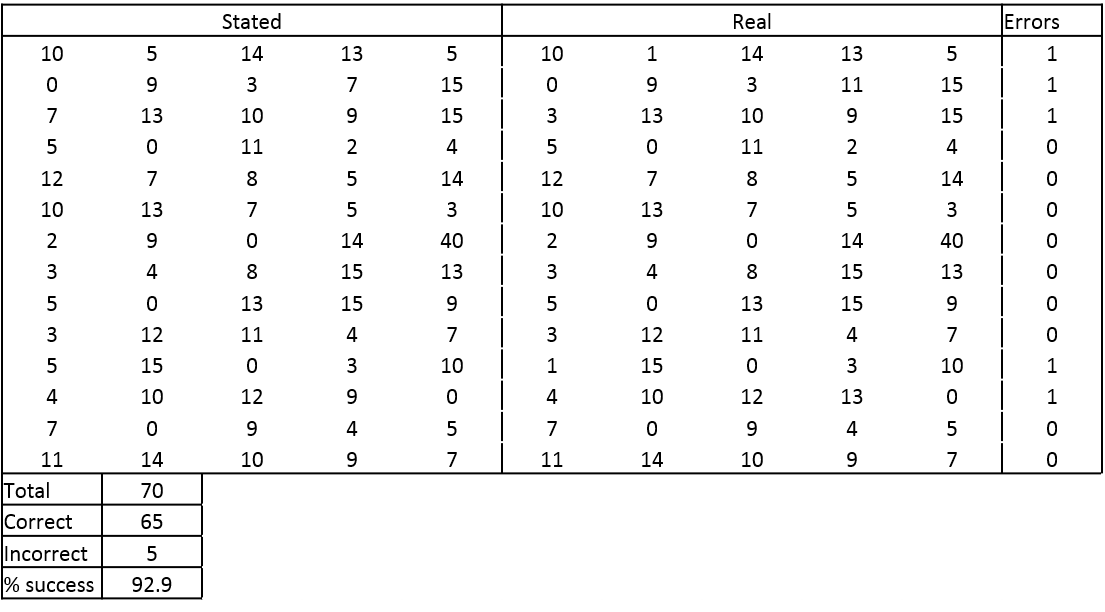
\includegraphics[width=0.8\textwidth]{images/gestureTableResults.png}
\captionof{figure}{Recorded Gesturing Effectiveness Results}
\label{figure:gestureResults}
\end{center}

\end{document}